\chapter{Higgs Plus Jets with Finite Quark Mass Effects}

%Chapter about work on getting the impact factor in $qg \to qgH$ relaxing our assumption that the Higgs is far from the gluon in rapidity and keeping the full dependence on the top mass. Focus on how the HE and infinite top mass limits commute, so this is `simple' to include. Also include interference with bottom quark loops. References to \cite{Duca2003}, \cite{DelDuca2001}, \cite{Hahn1999}. Approximately 40\% done, since the document describing how the amplitude is derived is still being written. 

It was briefly discussed at the end of section 2.3.2 that the addition of particles not charged under QCD, such as the $W^\pm$, $Z$ and Higgs bosons, are included in HEJ by deriving a modified current that encodes the emission of the boson. In this chapter, we look more closely at how this is done for the case of the Higgs boson in various limits. We will begin with the limit where the Higgs boson is emitted far apart from all other partons in rapidity and where the top quark mass is taken to infinity (the `infinite top mass limit'). Then we will relax the rapidity assumption on the Higgs and allow it to be produced close to an extremal parton in rapidity. Once this is established, we will consider the same rapidity situations without using the infinite top mass limit; this will constitute the author's own work. By the end of the chapter, we will have an expression that allows for the Leading Logarithmic resummation of Higgs plus at least two jets processes with full quark mass dependence, a calculation that is unique to HEJ.   
%\todo{Add new reference for bottom mass}
\section{The Infinite Top Mass Limit}
%HEJ `doesn't care' about whether the infinite top mass limit is implemented or not, so keeping full generality is `easy'. Discussion of why interference effects between top/bottom quark loops might be important (see, for example, \cite{Grazzini2013}).
%\todo{Also mention that it is important to describe tails correctly because of VBF cuts}

If we wish to place a Higgs boson along a rapidity chain consisting of $t$-channel gluon exchanges, then it would seem we would have to deal with loops. Since the gluon is massless, the first contribution to the $gg \to H$ vertex is at the one-loop level, where we have a massive quark loop that can couple to the Higgs directly. Loops generally complicate the calculation of an amplitude, so that even the calculation to leading order for this case is far more involved than a pure QCD process. This will be demonstrated further in the later sections of this chapter. In order to get around this complication, it is usual to take the limit where the top mass tends to infinity. This allows us to only consider a single quark loop (with the top quark) and then effectively shrink it down to a point, resulting in an \emph{effective} direct gluon-gluon-Higgs coupling in our Lagrangian\footnote{There is also a gluon-gluon-Higgs-Higgs interaction, but this thesis only concerns itself with single Higgs production, so we omit it for brevity here.} 
\begin{equation}
\mathscr{L}_{QCD + ggH} = \mathscr{L}_{QCD} + \frac{A}{4} G^{\mu \nu}G_{\mu \nu}H,
\end{equation}
with $A = \frac{\alpha_s}{3 \pi v}$ \cite{Duca2003} and where $G^{\mu \nu}$ is the field tensor for the gluon. This results in the following Feynman rule for the effective $ggH$ vertex \cite{Andersen2009a}
\begin{equation}
V_H^{\mu \nu}(q_1, q_2) = A \left( \eta^{\mu \nu} q_1 \cdot q_2 - q_1^\nu q_2^\mu \right),
\end{equation}
where $q_1$ is incoming to the vertex and $q_2$ outgoing. The simplest amplitude we can imagine is $qQ \to qHQ$, which has only one Feynman diagram: it is almost the same as the diagram for $qQ \to qQ$ scattering (figure \ref{fig:qQqQ}), with the only difference being the addition of the $ggH$ vertex along the $t$-channel gluon. It will be useful to absorb part of the expression for the $ggH$ vertex into the spinor chain, such that we create the object
\begin{equation}
S_{qQ \to qHQ}(q_1, q_2) = \matel{1}{\mu}{a} (\eta^{\mu \nu}q_1 \cdot q_2 - q_1^\nu q_2^\mu)\matel{2}{\nu}{b}. 
\end{equation} %I am sure of the 3 pi v here
With this, we can express the $qQ \to qHQ$ amplitude (summed and averaged over helicity and colour and exact within the infinite top mass limit) as
\begin{equation}
\begin{split}
|M_{qQ \to qHQ}|^2 &= \frac{1}{4(N_C^2 - 1)} ||S_{qQ \to qHQ}(q_1, q_2)||^2 \\
& \cdot \left(g^2 C_F \frac{1}{\hat{t}_1} \right) \\
& \cdot \left(\frac{1}{\hat{t}_1} \left(\frac{\alpha_s}{3 \pi v} \right)^2 \frac{1}{\hat{t}_2} \right) \\
& \cdot \left(g^2 C_F \frac{1}{\hat{t}_2} \right).
\end{split}
\end{equation}
If we wish to extend the result to other incoming states and/or with extra emissions, then we must also impose the condition that the Higgs boson is produced centrally and far away in rapidity from all other partons. Assuming that, we can once more insert Lipatov vertices and colour factors as appropriate. However, if we do not make this assumption then we are in a similar situation to the case of the unordered gluon in section 3.2 -- there are more terms in the amplitude that we cannot ignore. Furthermore, in contrast to the unordered case, this contribution is not suppressed in the MRK limit since the position of the Higgs boson along (or outside of) the rapidity chain does not change the colour properties of the amplitude. Such contributions must be taken into account. These are included in HEJ via the use of impact factors \cite{Duca2003}, which are strict high energy expressions that include all relevant terms in this limit.   

The infinite top mass limit is remarkably successful for predictions of inclusive variables like total cross sections. The reason for this is that the expansion of this effective coupling is a power series in $\frac{m_H^2}{4 m_t^2} \sim 0.13$ and we assume the top mass is the most relevant scale in the problem. In \cite{Duca2003}, it was shown that even the addition of a large dijet invariant mass in the amplitude has little effect. However, if the transverse scales start to become larger than the top mass (in particular, the transverse scales of the gluons entering the effective vertex), there is significant deviation between the result obtained in the full and effective theories \cite{Duca2003}. 

For HEJ, the infinite top mass limit was included as a first approximation, but the factorisation of amplitudes will still occur whether or not this limit is taken. Therefore, any derived vertices for Higgs production with the full quark mass included can still be implemented in a straightforward way. Furthermore, as soon as the vertex including the full quark mass is derived, we can trivially add in the effect of more than one quark loop (for example, where a bottom quark runs in the loop). Such interference has been shown to produce interesting effects at small $p_T$ scales, at least in processes involving the emission of a Higgs boson with one accompanying jet \cite{Grazzini2013, Lindert2017}. For these reasons, it is important to include the effect of finite quark masses in the HEJ formalism. Finally, since the emission of extra jets is trivial in HEJ, the inclusion of a full finite-quark-mass-dependent expression for the $gg \to H$ coupling will result in a prediction for the $pp \to H + n$ jets amplitude for any $n$ without the assumption of a infinite top mass. This is a calculation that is far beyond the reach of any fixed-order approach. 

\section{Calculations of $H$ + Jets with Finite Quark Mass Effects}

As previously discussed, there are two rapidity cases to be discussed: the first where the Higgs is emitted centrally and the second where it is emitted outside of an extremal parton. The base amplitude for the first is the $qQ \to qHQ$ amplitude, which we will discuss in the next subsection. For the case where the Higgs is emitted outside of an extremal parton, we look at the $gq \to Hgq$ amplitude, where the Higgs boson is emitted outside of the gluon. Such a process gives rise to diagrams involving box integrals which become important in this limit, making the study of amplitudes involving the Higgs emitted outside of an extremal gluon fundamentally different. 

\subsection{$qQ \to qHQ$}

The expression for the $qQ \to qHQ$ amplitude with full finite quark mass effects is shown diagrammatically in figure \ref{fig:qQh_eff}. In the previous section, we showed how the amplitude was derived in the infinite top mass limit. Because the factorisation properties of the amplitude are unchanged by moving away from this limit, the extension of this amplitude to the full (finite quark mass dependent) amplitude is found by simply `undoing' the infinite top mass limit in the vertex $V_H^{\mu \nu}$. Such an expression can be found, for example in Appendix B of \cite{Duca2003}, so long as care is taken to ensure that incoming and outgoing momenta are labelled correctly. Keeping with the convention before that $q_1$ is incoming and $q_2$ outgoing, the vertex with a finite top mass is
\begin{equation}
V^{\mu \nu}_{H, m_t}(q_1, q_2) = -\frac{4 g_s^2 m_t^2}{v} \left[\eta^{\mu \nu}A_2(-q_1,q_2) + q_1^\nu q_2^\mu A_1(-q_1,q_2) \right],
\end{equation}
\begin{figure}[t]
\centering
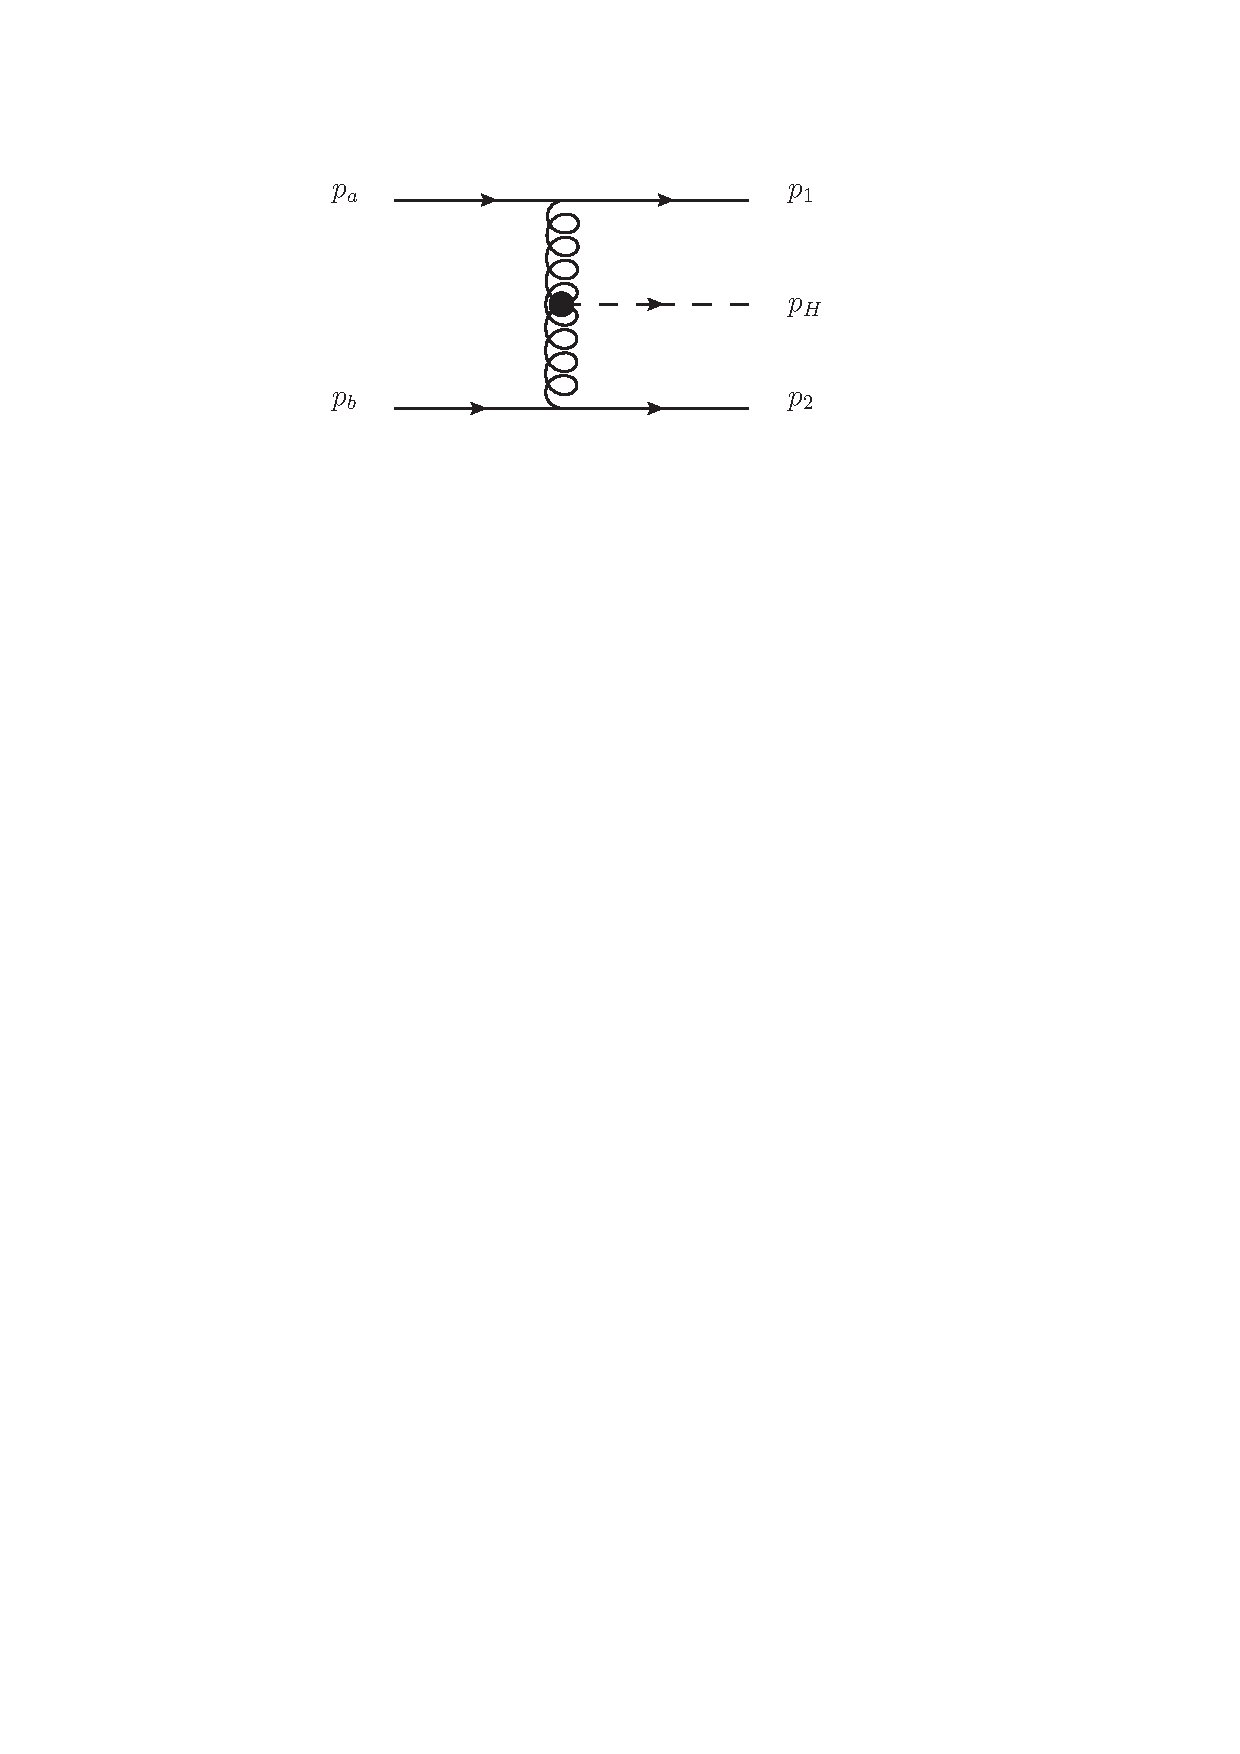
\includegraphics{Images/qQh_eff.pdf}
\caption{Diagrammatic representation of $qQ \to qHQ$ with an effective vertex for the production of the Higgs.}
\label{fig:qQh_eff}
\end{figure}

where $v$ is the Higgs vacuum expectation value ($\approx 246$ GeV) and $A_1, A_2$ depend on a combination of scalar integrals which appear via the integral reduction technique \cite{Chetyrkin1981}. We first define\footnote{The integral $B_0$ is actually divergent in 4 dimensions, but will always appear in combinations such that this divergence cancels in later functions.}
\begin{equation}
\begin{split}
B_0(k) &= \int \frac{d^4 q}{(2 \pi)^4} \frac{1}{(q^2-m_t^2)((q+k)^2-m_t^2)}, \\
C_0(p,k) &= \int \frac{d^4 q}{(2 \pi)^4} \frac{1}{(q^2-m_t^2)((q+p)^2-m_t^2)((q+p+k)^2-m_t^2)}, \\
Q &= -q_1 - q_2, \\
\Delta_3 &= (q_1^2)^2 + (q_2^2)^2 + (Q^2)^2 - 2 q_1^2 q_2^2 - 2q_1^2Q^2 - 2q_2^2Q^2,
\end{split}
\label{eqn:scalars}
\end{equation}
which allows us to give the forms of $A_1$ and $A_2$ as
\begin{equation}
\begin{split}
A_1(-q_1,q_2) &= C_0(-q_1,q_2) \left[\frac{4 m_t^2}{\Delta_3}(Q^2-q_1^2-q_2^2)-1-\frac{4q_1^2q_2^2}{\Delta_3} - \frac{12q_1^2q_2^2Q^2}{\Delta_3^2}(q_1^2+q_2^2-Q^2) \right] \\
&- \left[B_0(q_2)-B_0(Q) \right] \left[\frac{2 q_1^2}{\Delta_3} + \frac{12 q_1^2 q_2^2}{\Delta_3^2}(q_2^2-q_1^2+Q^2) \right] \\
& - \left[B_0(-q_1)-B_0(Q) \right] \left[\frac{2q_1^2}{\Delta_3} + \frac{12 q_1^2 q_2^2}{\Delta_3^2}(q_1^2-q_2^2+Q^2) \right] \\
& - \frac{2}{\Delta_3} \frac{i}{(4 \pi)^2}(q_1^2 + q_2^2 - Q^2) \\
A_2(-q_1,q_2) &=  C_0(-q_1,q_2) \left[2 m_t^2 + \frac{1}{2}(q_1^2+q_2^2-Q^2) + \frac{2 q_1^2 q_2^2Q^2}{\Delta_3} \right] \\
&+ \left[B_0(q_2)-B_0(Q) \right] \frac{1}{\Delta_3}q_2^2(q_2^2-q_1^2-Q^2) \\
& + \left[B_0(-q_1)-B_0(Q) \right] \frac{1}{\Delta_3}q_1^2(q_1^2-q_2^2-Q^2)\\
& +\frac{i}{(4 \pi)^2}.
\label{eqn:afuncs} 
\end{split}
\end{equation}
The scalar integrals can either be evaluated numerically (via, for example, a program like LoopTools \cite{Hahn1999}) or again simply looked up,\footnote{It is important to realise that most given results are valid only in certain kinematical regions, so care must be taken to pick the correct analytical formula.} so that the values of $A_1$ and $A_2$ can be determined at any point. It can be numerically checked that
\begin{equation}
\begin{split}
\lim_{m_t \to \infty} 4 \frac{g_s^2 m_t^2}{v}A_1(-q_1,q_2) &= i A, \\
\lim_{m_t \to \infty} 4 \frac{g_s^2 m_t^2}{v}A_2(-q_1,q_2) &= -i q_1 \cdot q_2 A, \\
\end{split}
\end{equation}
and thus
\begin{equation}
\lim_{m_t \to \infty}V^{\mu \nu}_{H, m_t} \to -i V^{\mu \nu}_H,
\end{equation}
where the phase factor of $-i$ arises from a difference in convention and is unimportant since we are always taking the modulus squared of the amplitude. We can therefore simply insert this vertex rather than the infinite top mass vertex into our amplitude to get the result
\begin{equation}
\begin{split}
|M_{qQ \to qHQ}^{HE,ggH}|^2 &= \frac{1}{4(N_C^2 - 1)} ||S_{qQ \to qHQ}^{\hspace{2pt} m_t}(q_1, q_2)||^2 \\
& \cdot \left(g^2 C_F \frac{1}{\hat{t}_1} \right) \\
& \cdot \left(\frac{1}{\hat{t}_1} \left(\frac{-4 g_s^2 m_t^2}{v} \right)^2 \frac{1}{\hat{t}_2} \right) \\
& \cdot \left(g^2 C_F \frac{1}{\hat{t}_2} \right)
\end{split}
\end{equation}
with
\begin{equation}
S_{qQ \to qHQ}^{\hspace{2pt} m_t}(q_1, q_2) = \matel{1}{\mu}{a} (\eta^{\mu \nu}A_2(-q_1,q_2) + q_1^\nu q_2^\mu A_1(-q_1,q_2))\matel{2}{\nu}{b}. 
\end{equation} 
To see how much of a difference this makes to the amplitude, we plot the results for the infinite and finite top mass cases in figure \ref{fig:qHQ_comp}. The momenta used are the following:
\begin{subequations}
\begin{align}
p_1 &= (40 \sqrt{2} \cosh(\Delta),-40,40,40 \sqrt{2} \sinh(\Delta)), \\
p_H &= (\sqrt{40^2+m_H^2}, 0,-40,0), \\
p_2 &= (40 \cosh(-\Delta),40,0,40 \sinh(-\Delta)).
\end{align}
\end{subequations}
The two results agree well until around $\Delta = 3$ when they begin to split. In the High Energy Limit, the finite top mass result is larger than the infinite top mass result by about $3\%$. 
\begin{figure}[t]
\centering
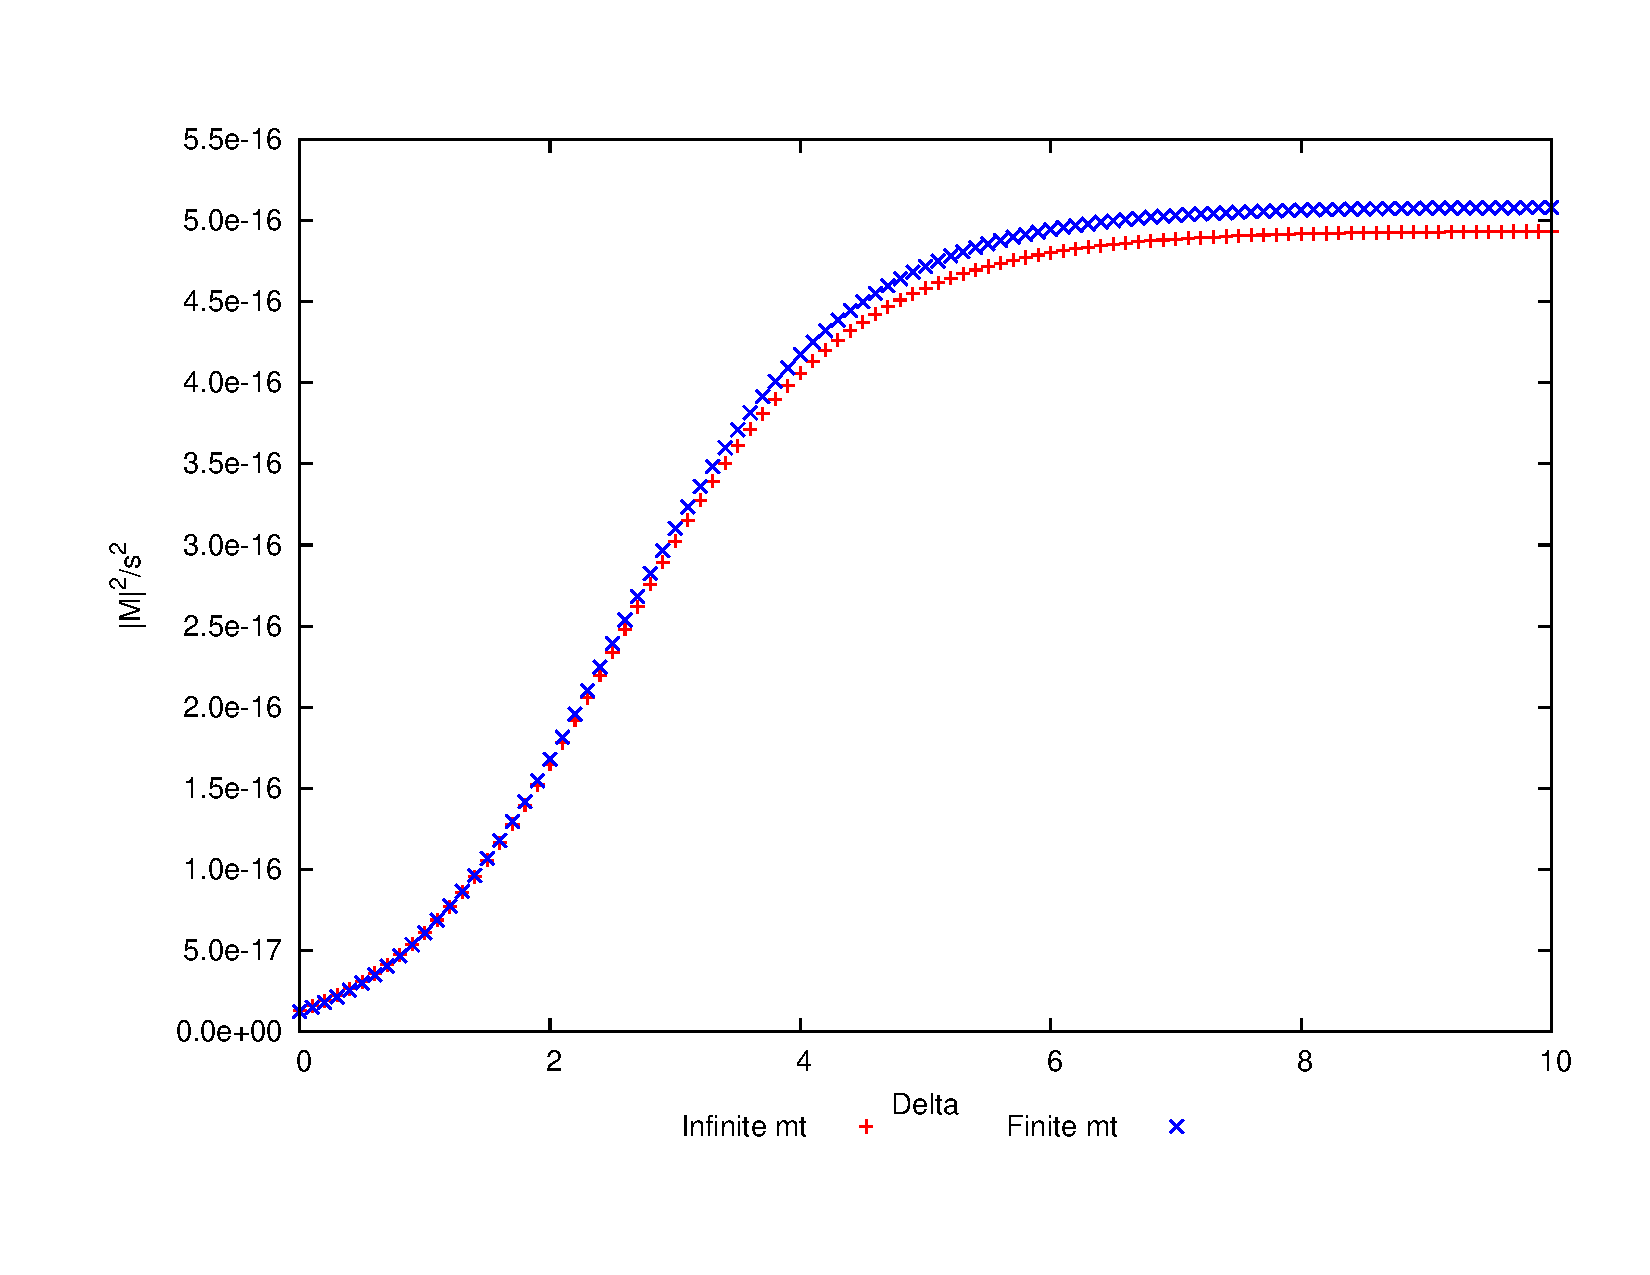
\includegraphics[scale=0.5]{Images/qQ_qHQ_comp.pdf}
\caption{Behaviour of the $ud \to uHd$ amplitude in a slice of phase space where the Higgs boson is kept central in rapidity. The red line shows the result for the matrix element when the infinite top mass limit is taken and the blue line shows the result when the full top quark mass is taken into account.}
\label{fig:qHQ_comp}
\end{figure}

\subsection{$gq \to Hgq$}

The situation where the Higgs is emitted outside of an extremal gluon involves a much more thorough calculation. We will start by finding the general leading order expression and then use knowledge of the high energy limit considered ($y_H \sim y_1 \gg y_2$) to again factorise the expression into the form HEJ requires, shown schematically in figure \ref{fig:gqH_imp} and of the form
\begin{equation}
M \sim \frac{Z^{\mu}(p_a,p_1,p_H) \matel{2}{\mu}{b}}{\hat{t}_2},
\label{eqn:higgseff}
\end{equation}
\begin{figure}[t]
\centering
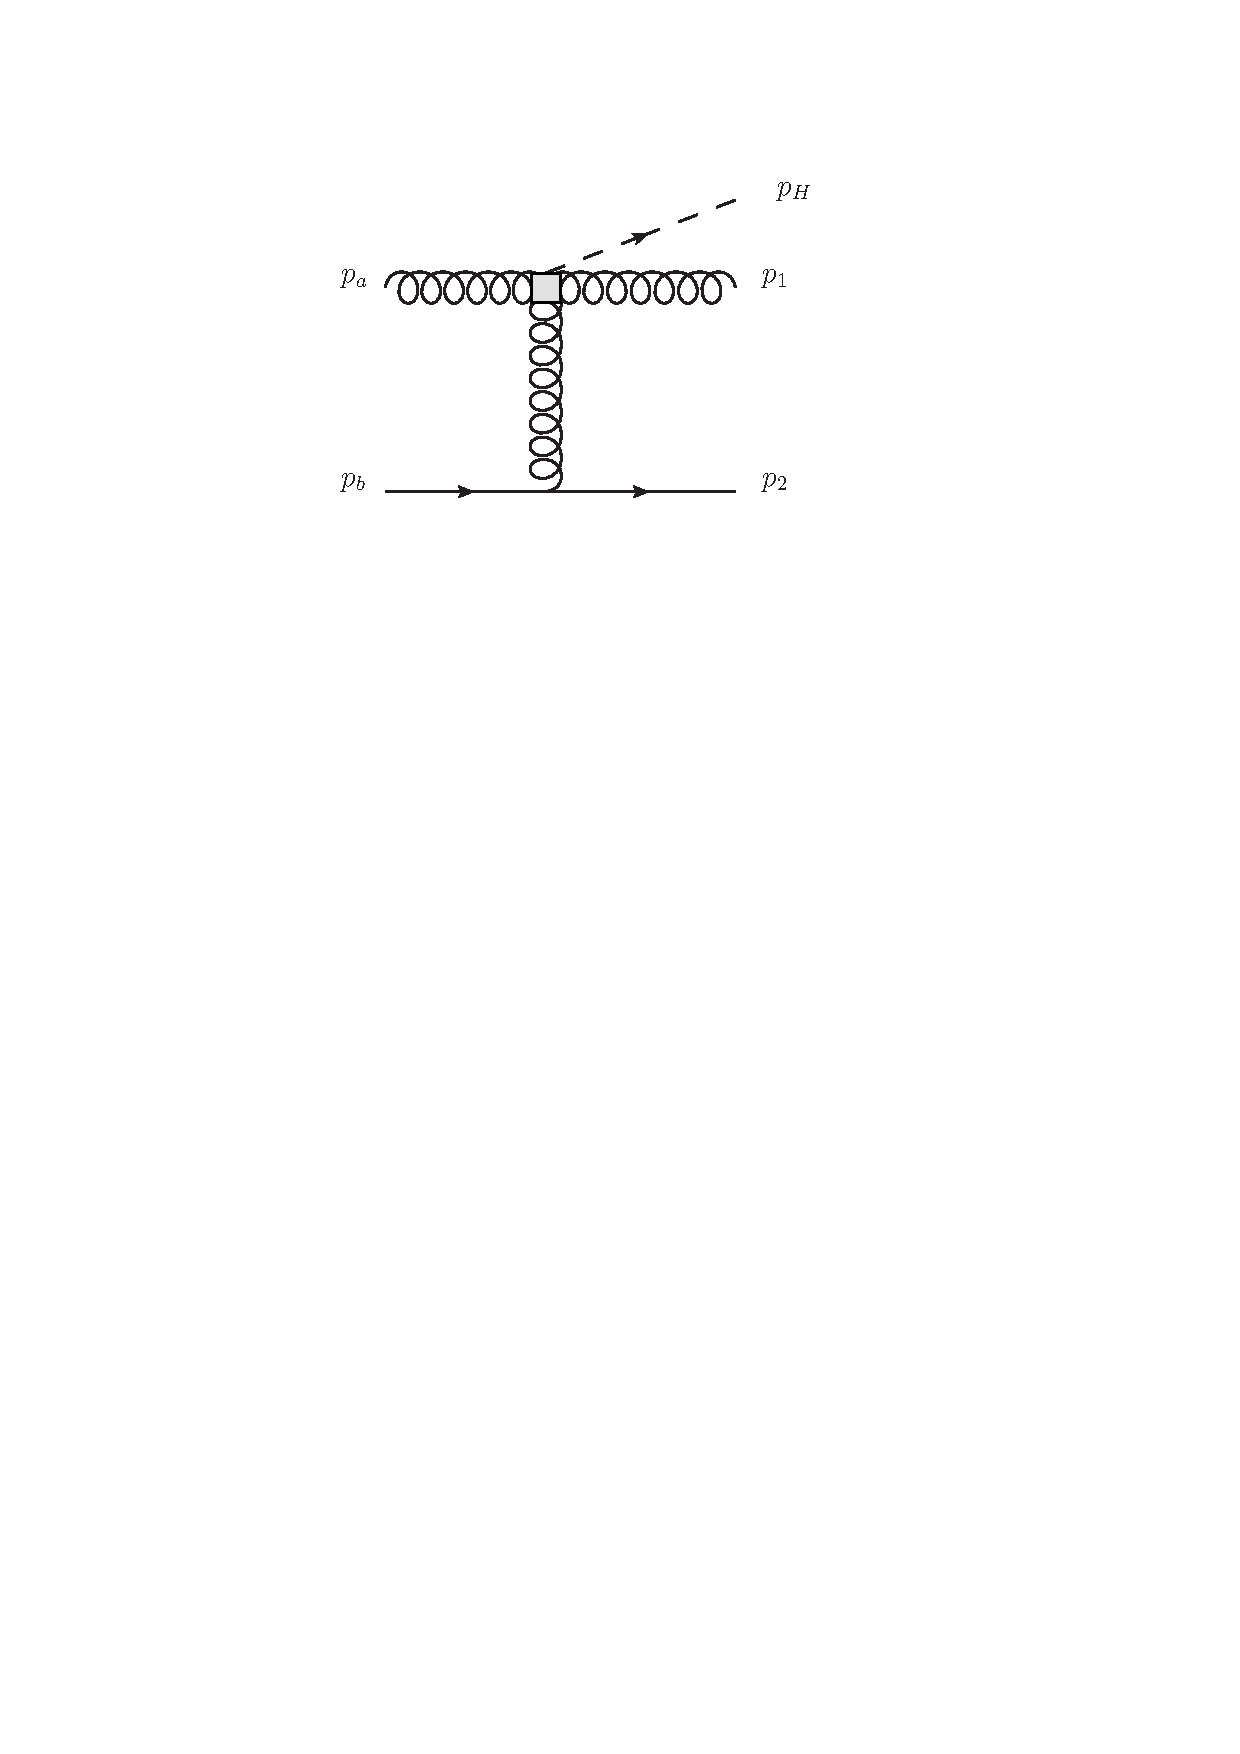
\includegraphics{Images/qgh_impact_factor.pdf}
\caption{Diagrammatic representation of factorised $gq \to gHq$ expression.}
\label{fig:gqH_imp}
\end{figure}

assuming that the polarisation vectors of the external gluons have been contracted with the effective vertex. Here, $\hat{t}_2 = p_2 - p_b$ is the $t$-channel pole we will resum (the definition of $\hat{t}_i$ used in the previous chapter no longer holds here since we have an extra momentum to consider). There are 20 leading order diagrams to consider in total, which is reduced to 10 after invoking Furry's Theorem \cite{Atkin2015}, which states that diagrams involving an anti-quark loop can be related to diagrams with a quark loop. A selection of these diagrams is shown in figure \ref{fig:qgh_lo}. We will use \cite{DelDuca2001} as a guide for our work. We begin by finding a suitable parametrisation for the triangle graphs that appear in the amplitudes. Using Furry's Theorem, we find that we can describe these graphs (one with a quark running around the loop and the other with an anti-quark) using only one object, $T^{\mu_1 \mu_2}(q_1,q_2)$. Gauge invariance of these graphs implies $q_1^{\mu_1} T_{\mu_1 \mu_2} = q_2^{\mu_2}T_{\mu_1 \mu_2} = 0$, and so the generic tensor structure is
\begin{equation}
T^{\mu_1 \mu_2} (q_1, q_2) = F_T(q_1^2, q_2^2,(q_1+q_2)^2) T_T^{\mu_1 \mu_2} + F_L(q_1^2, q_2^2,(q_1+q_2)^2) T_L^{\mu_1 \mu_2},
\end{equation}
\begin{figure}[t] 
\centering
\subfloat{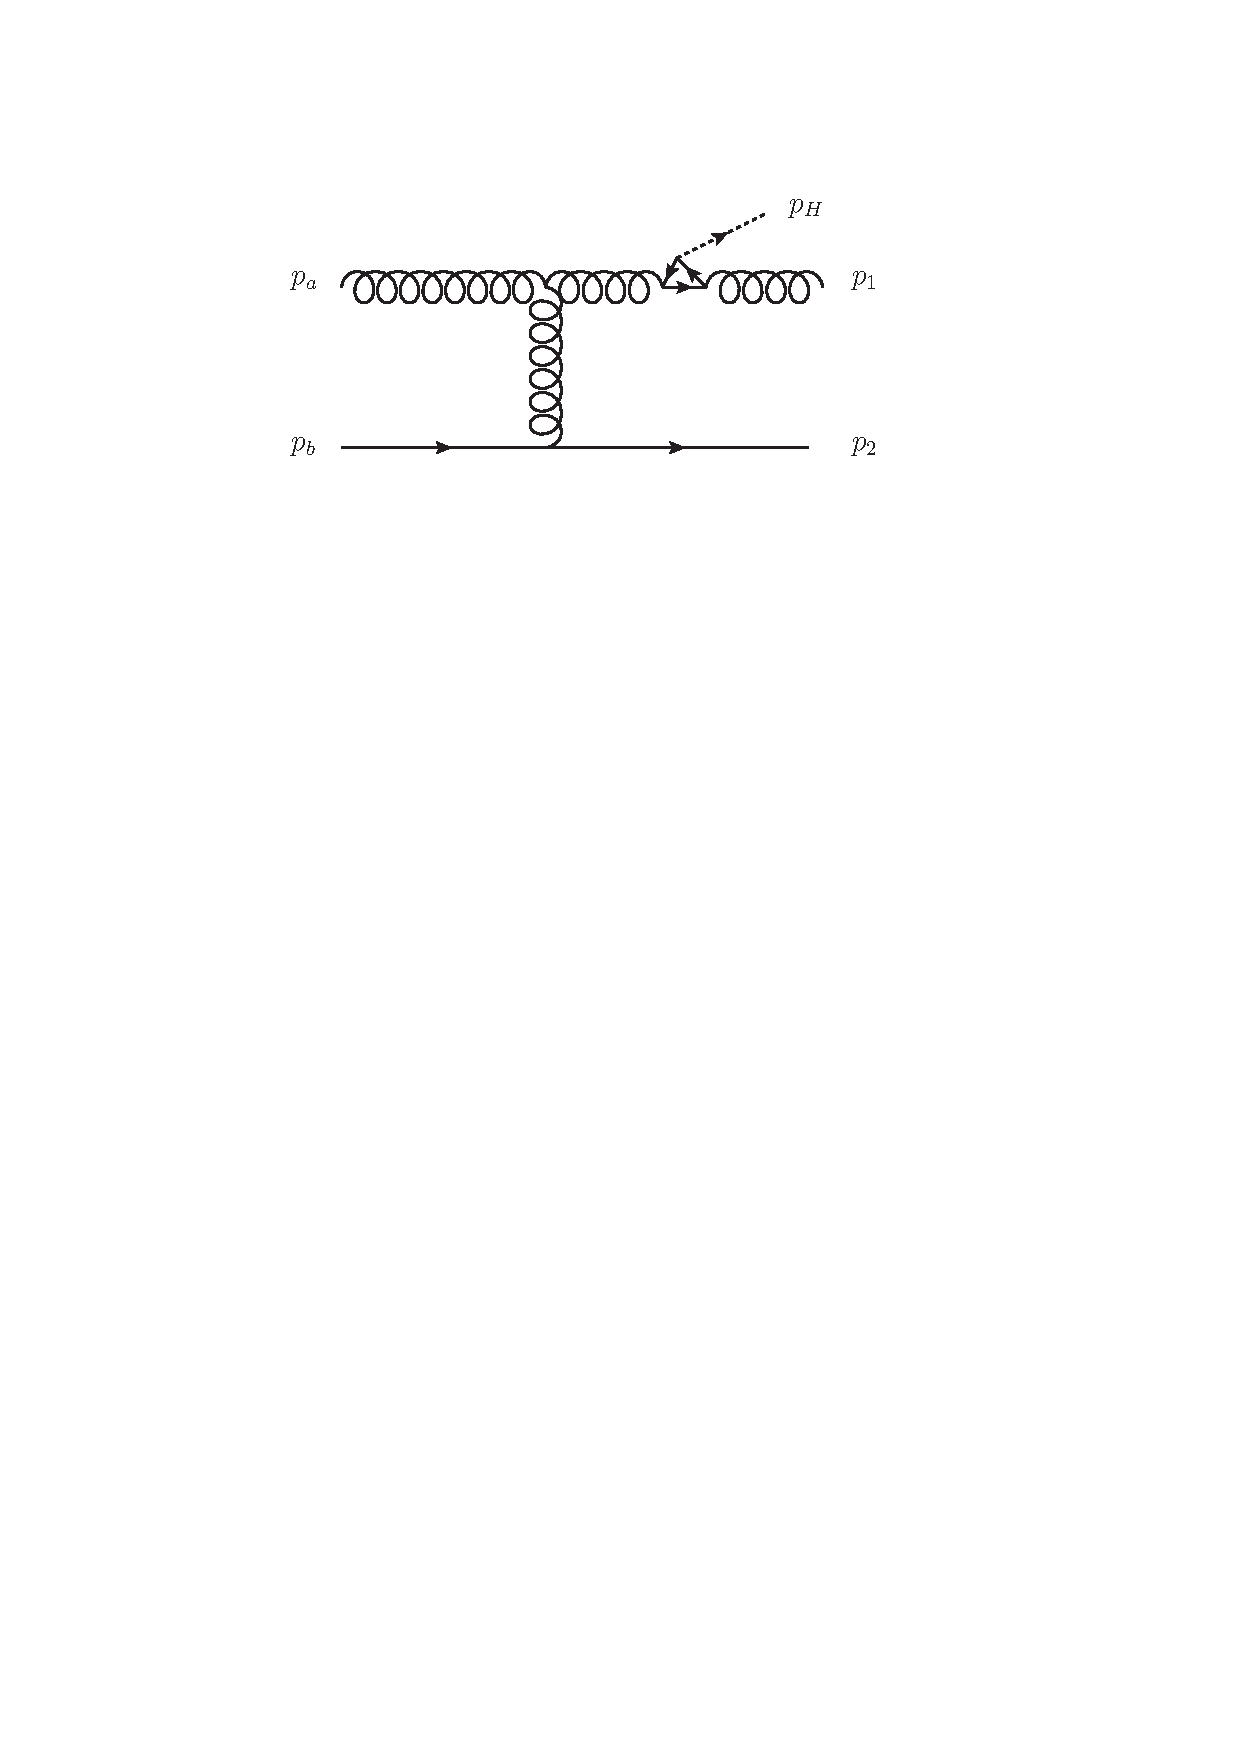
\includegraphics[scale=0.75]{Images/qgh_pa_t.pdf}} 
\subfloat{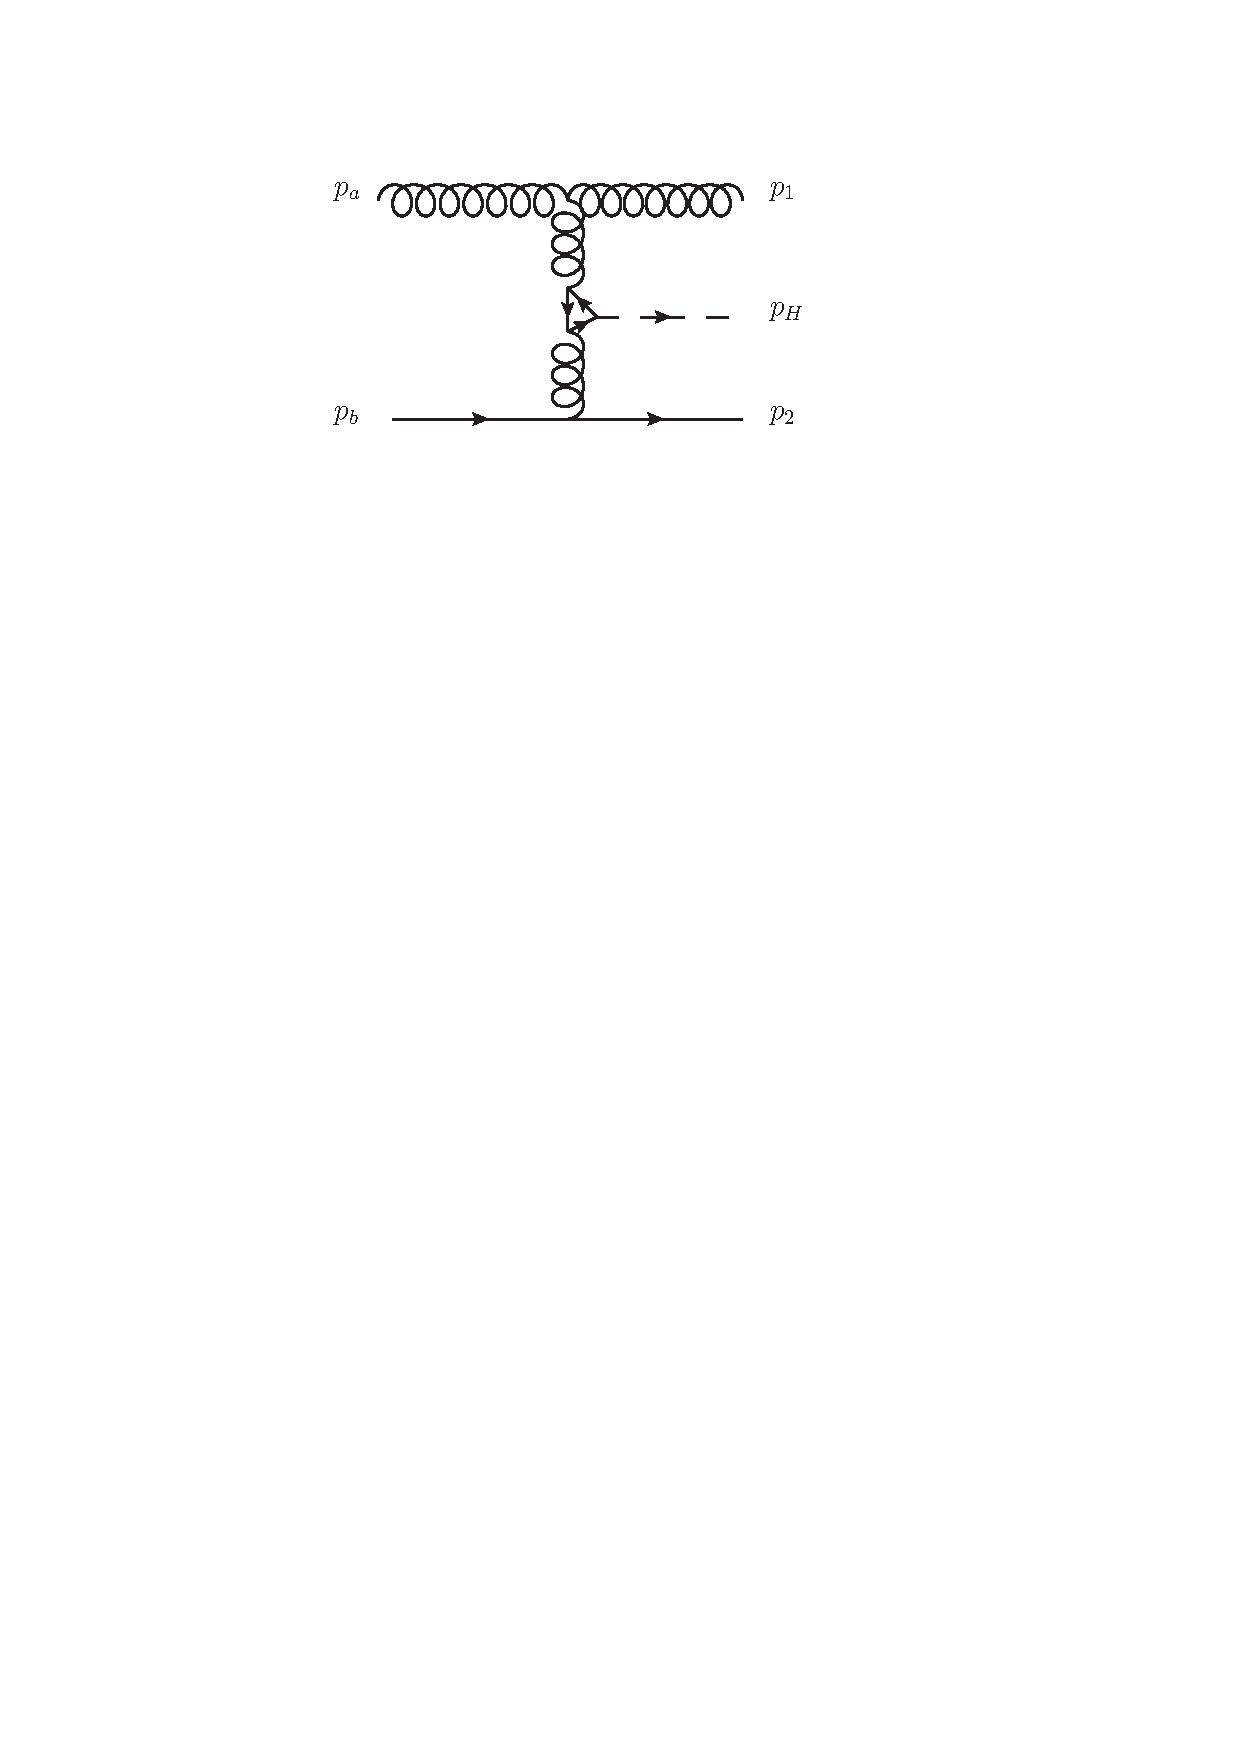
\includegraphics[scale=0.75]{Images/qgh_middle.pdf}} \\
\subfloat{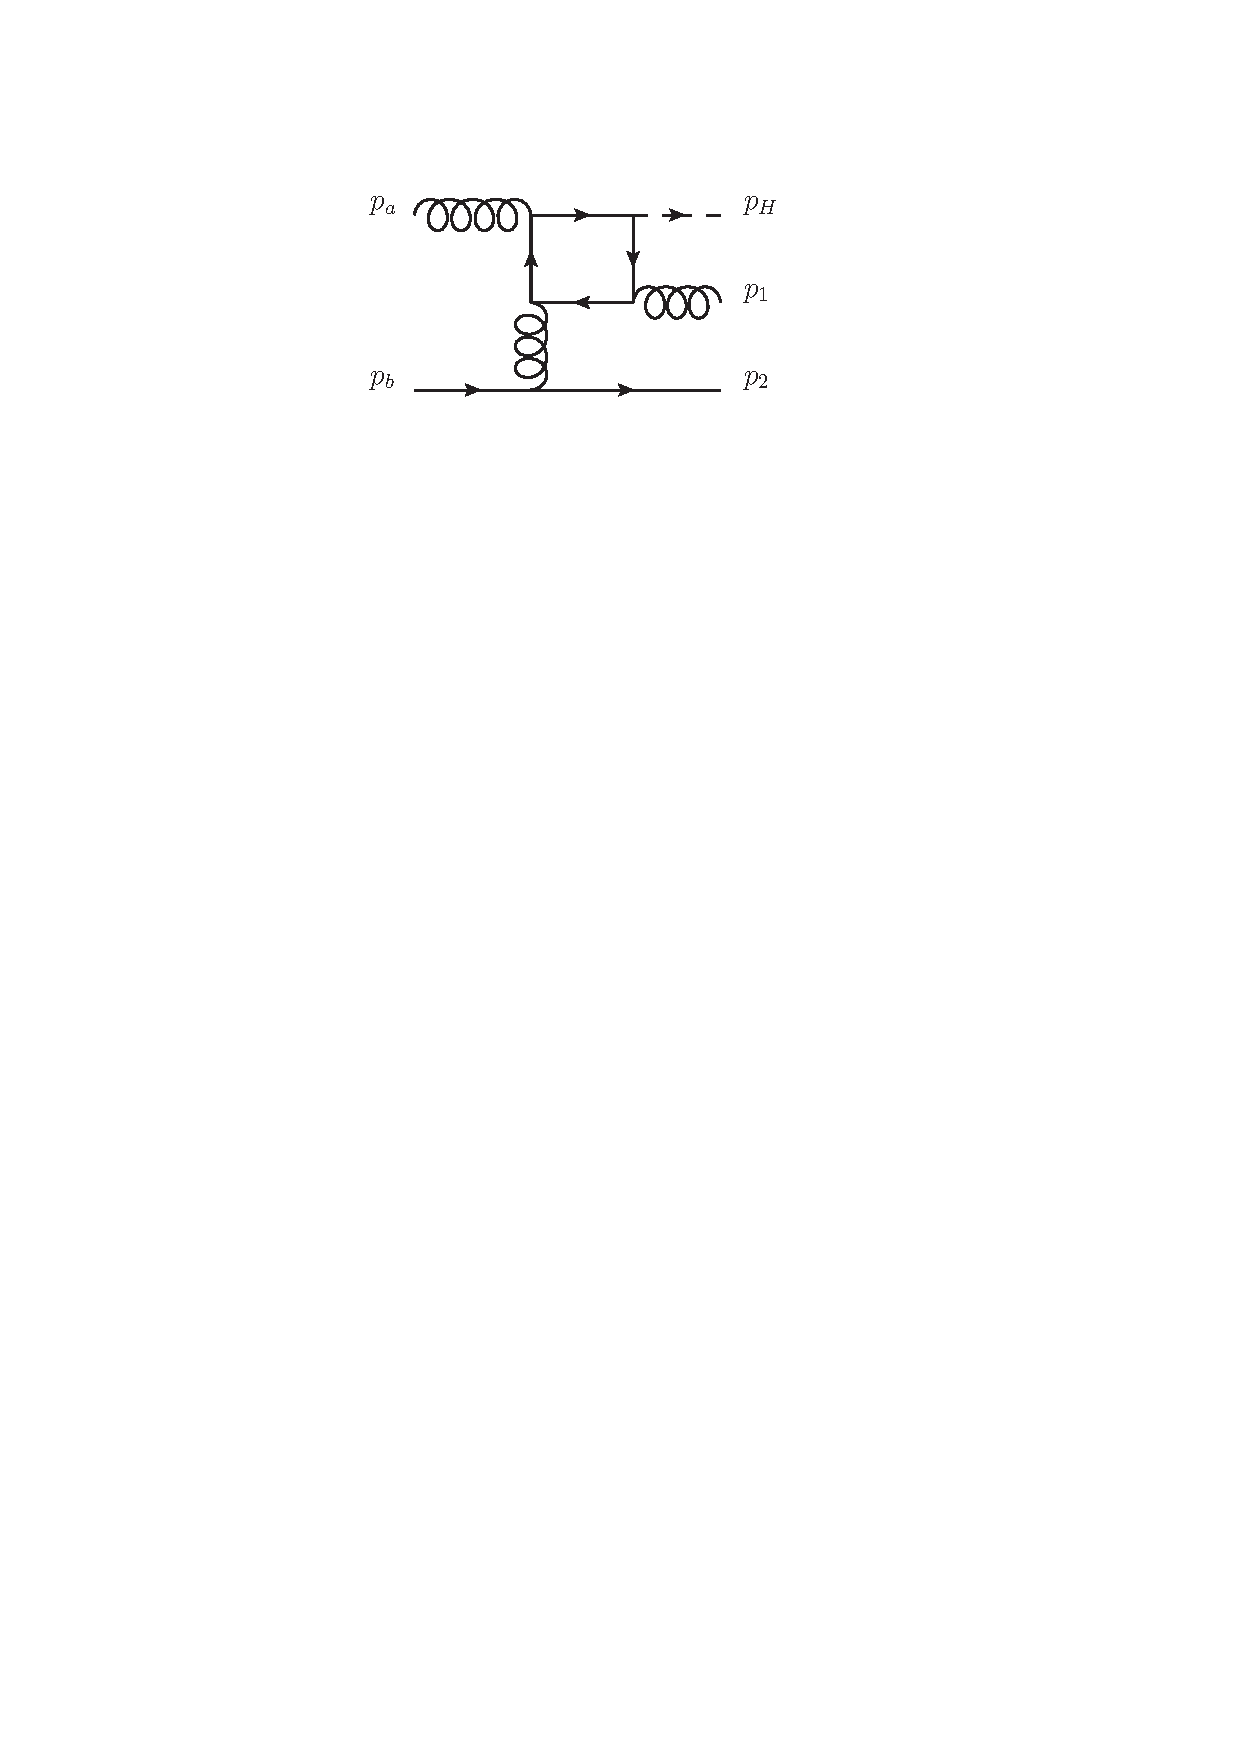
\includegraphics[scale=0.75]{Images/box.pdf}} 
\subfloat{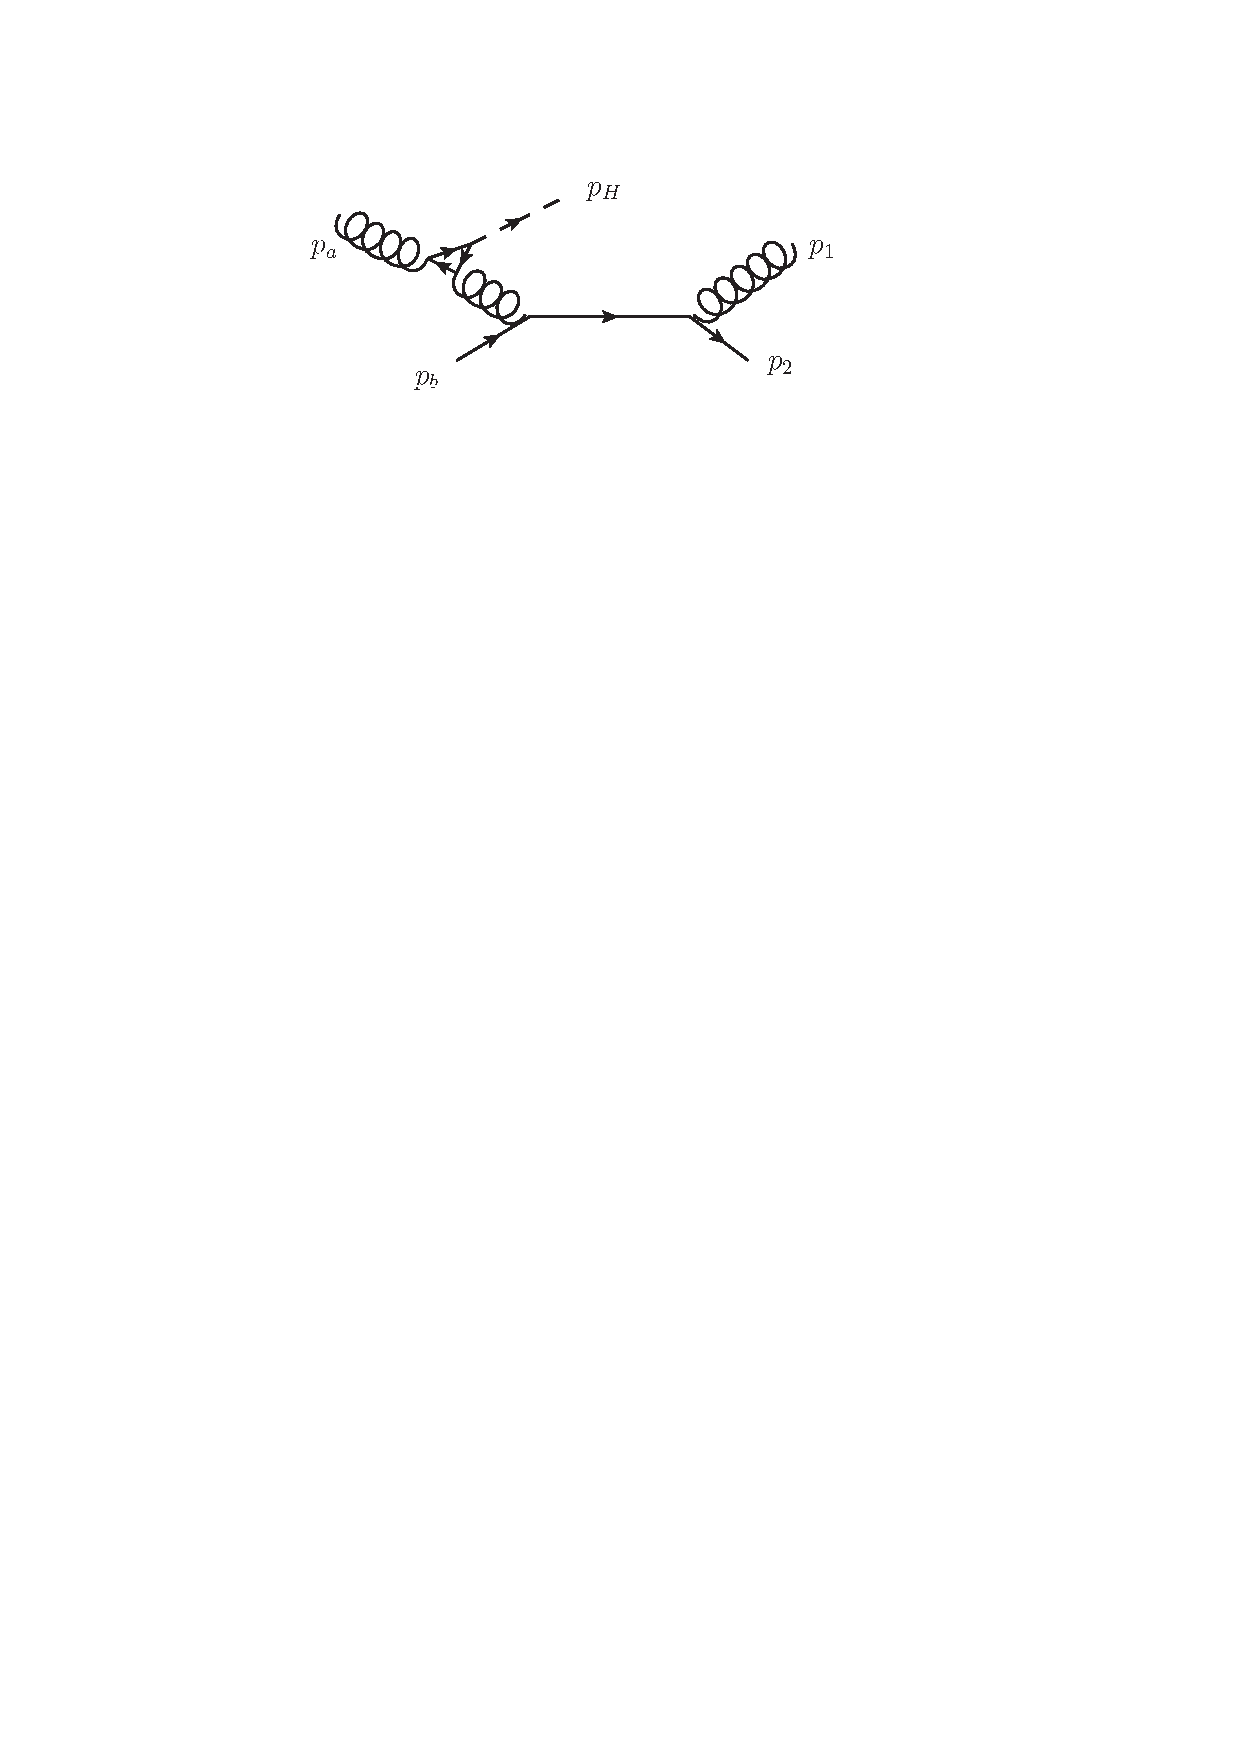
\includegraphics[scale=0.75]{Images/qgh_s.pdf}} \\
\subfloat{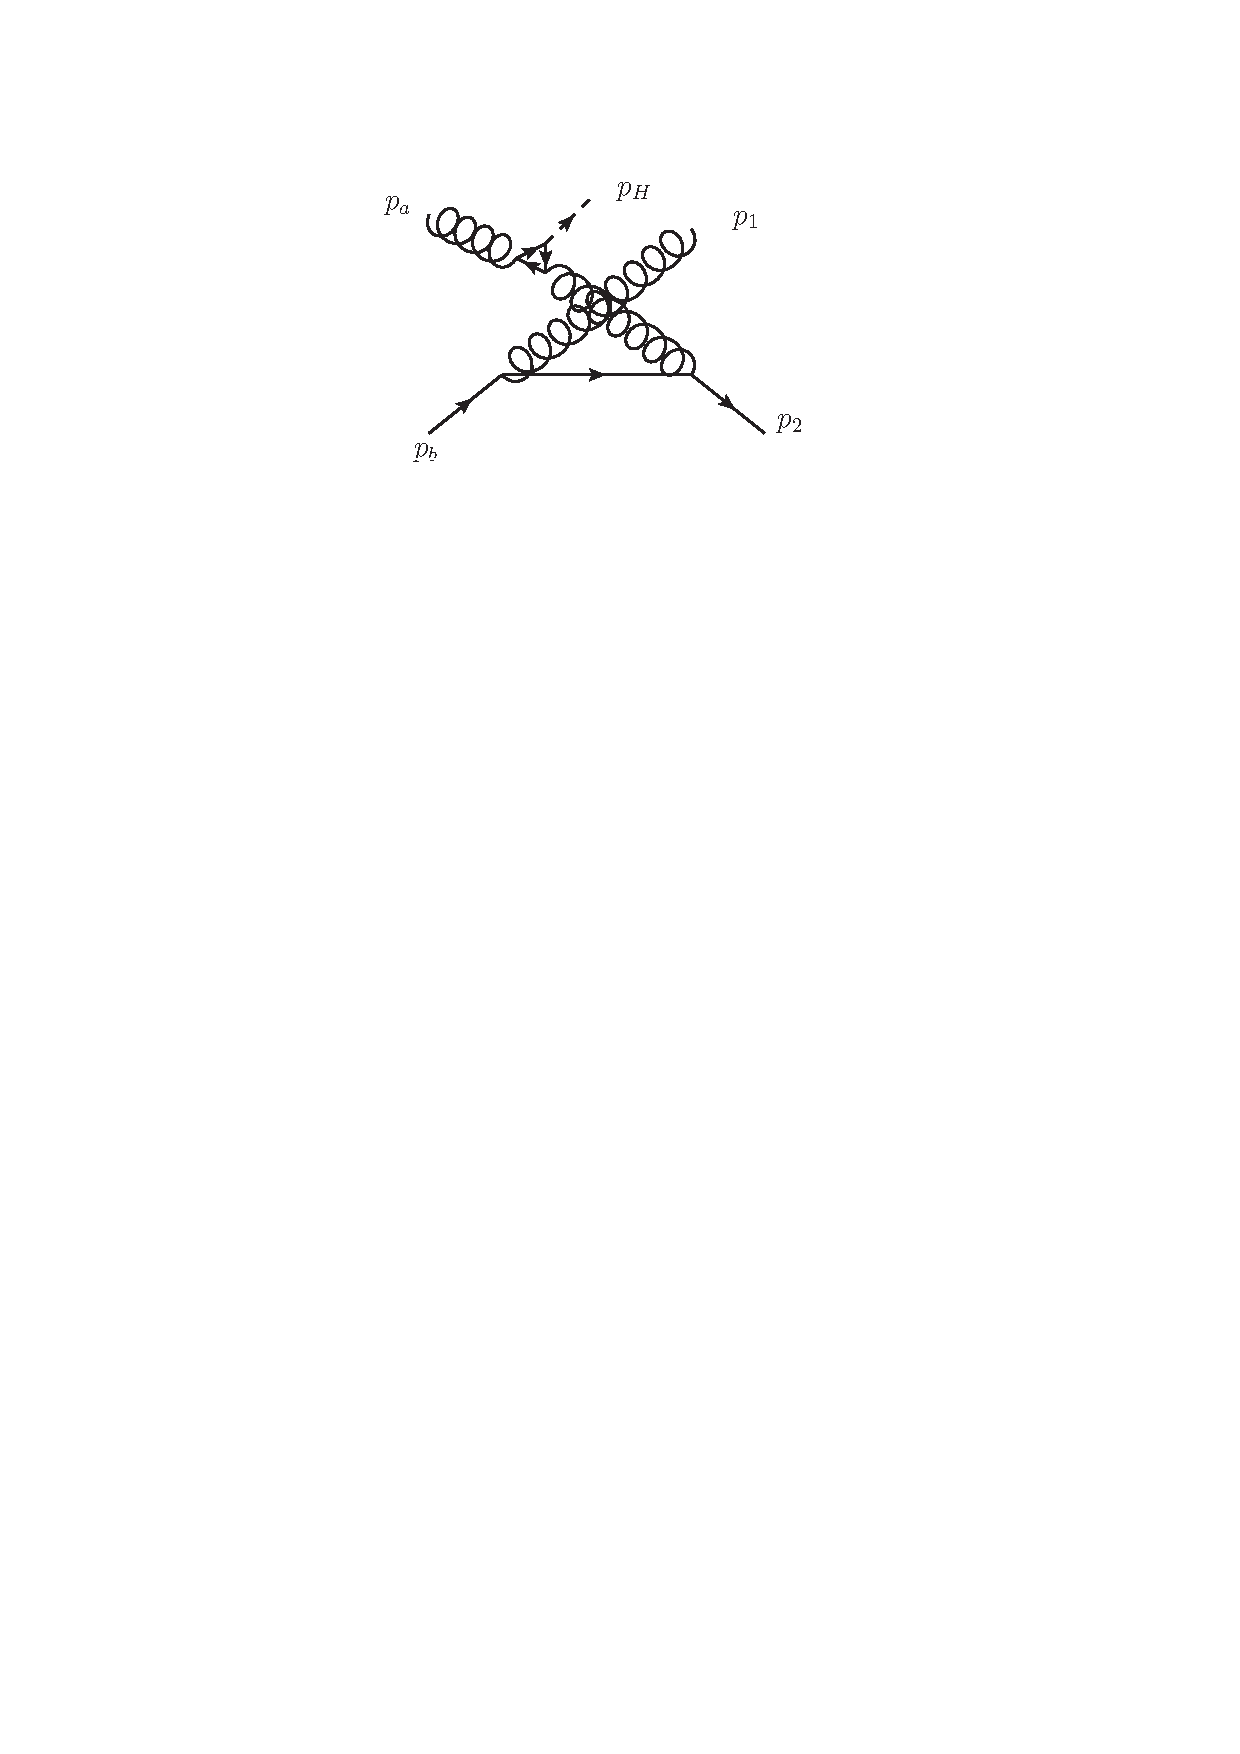
\includegraphics[scale=0.75]{Images/qg_qgh_u.pdf}}
\caption{A selection of LO graphs for $gq \to Hgq$.}
\label{fig:qgh_lo}
\end{figure}
%\todo{Make this nicer, perhaps add a few more. All 10 graphs, maybe? Or 8, if we just have one box.}
where $ T_T^{\mu_1 \mu_2} = q_1 \cdot q_2 \eta^{\mu_1 \mu_2} - q_1^{\mu_2} q_2^{\mu_1} $ and $T_L^{\mu_1 \mu_2} = q_1^2 q_2^2 \eta^{\mu_1 \mu_2} - q_1^2 q_2^{\mu_1} q_2^{\mu_2} - q_2^2 q_1^{\mu_1} q_1^{\mu_2} + q_1 \cdot q_2 q_1^{\mu_1} q_2^{\mu_2}$, and both $q_1$ and $q_2$ are going out from the triangle loop\footnote{In our calculation, we will not conform to this convention and so we will take care with signs here.}. The full forms for the $F_L$ and $F_T$ functions are
\begin{equation}
\begin{split}
F_L(q_1^2,q_2^2,Q^2) &= -\frac{1}{2 \text{det} \mathcal{Q}_2} \bigg \{ \left[2-\frac{3 q_1^2 q_2 \cdot Q}{2 \text{det}\mathcal{Q}_2} \right] \left(\tilde{B}_0(q_1)-\tilde{B}_0(Q) \right)\\
&+ \left[2-\frac{3 q_2^2 q_1 \cdot Q}{2 \text{det}\mathcal{Q}_2} \right] \left(\tilde{B}_0(q_2)-\tilde{B}_0(Q) \right) \\
&- \left[4m_t^2 + q_1^2 + q_2^2 + Q^2 - \frac{3 q_1^2 q_2^2 Q^2}{\text{det}\mathcal{Q}_2} \right] \tilde{C}_0(q_1,q_2) - 2 \bigg \}, \\
F_T(q_1^2, q_2^2, Q^2) &= -\frac{1}{2 \text{det} \mathcal{Q}_2} \bigg \{ Q^2 \left[\tilde{B}_0(q_1) + \tilde{B}_0(q_2) - 2\tilde{B}_0(Q) - 2 q_1 \cdot q_2 \hspace{2pt} \tilde{C}_0(q_1,q_2) \right] \\
&+ \left(q_1^2-q_2^2 \right) \left(\tilde{B}_0(q_1) - \tilde{B}_0(q_2)\right) \bigg \} - q_1 \cdot q_2 \hspace{2pt} F_L,
\end{split}
\end{equation}
where $\text{det} \mathcal{Q}_2 =q_1^2q_2^2 - (q_1 \cdot q_2)^2$. The scalar integrals with the tilde notation are equal to the scalar integrals shown in equation \ref{eqn:scalars} multiplied by $-16i\pi^2$. The $F_L$ and $F_T$ functions are related to the $A_1$ and $A_2$ of equation \ref{eqn:afuncs} by
\begin{equation}
\begin{split}
A_1(q_1,q_2) &= \frac{i}{(4 \pi)^2}F_T(q_1,q_2), \\
A_2(q_1,q_2) &= \frac{i}{(4 \pi)^2}\left(F_T(q_1,q_2) q_1 \cdot q_2 + F_L(q_1,q_2)q_1^2q_2^2 \right).
\end{split}
\end{equation}
An interesting point to notice is that, if one of the momenta $q_1$ or $q_2$ is on-shell, we only get a contribution from the transverse ($F_T$) term in $T^{\mu \nu}$. This comes about because the presence of an on-shell momenta must mean that the vertex is going to be contracted with the relevant polarisation vector, setting the longitudinal term ($F_L$) to zero. When this happens, we will write $T_R$ in place of $T$ to remind ourselves of this. Finally, since we know that every graph contributes at the same order in $\alpha_s$, has a Yukawa coupling from the top loop and has factors from loop integrals, we conveniently define
\begin{equation}
 F = \frac{4 m_t^2}{v} \alpha_s^2, 
\end{equation}
and multiply $F$ into every graph as in \cite{DelDuca2001}. This slightly changes the Feynman rules for QCD that we should use in that all coupling information is now factored out for convenience.

We now begin the process of finding the full LO expression. We start with the graph shown in the top left of figure \ref{fig:qgh_lo}, where the Higgs is emitted from the gluon leg with momentum $p_1$. The Feynman rules yield
\begin{equation}
\begin{split}
A_1 = -F \varepsilon_{\mu_1}(p_a)f^{a1t}V_{3g}^{\mu_1 \mu_2 \mu_3}(p_a, -p_1-p_H,-p_a+p_1+p_H)\left(\frac{-i \eta_{\mu_2 \mu_4}}{(p_1+p_H)^2}\right) \\
T_R^{\mu_4 \mu_5}(-p_1-p_H, p_1) \varepsilon^*_{\mu_5}(p_1)\left(\frac{-i \eta_{\mu_3 \mu_6}}{\hat{t}_2}\right)(-i)T^t_{2b}\matel{2}{\mu_6}{b},
\end{split}
\end{equation}
which can be simplified to give
\begin{equation}
\begin{split}
A_1 &= \frac{-i Ff^{a1t}T^t_{2b}}{(p_1+p_H)^2 \hat{t}_2} \varepsilon_{\mu_1}(p_a)V_{3g}^{\mu_1 \mu_2 \mu_3}(p_a, -p_1-p_H,-p_a+p_1+p_H) \\
&\cdot T_{R, \mu_2}^{\hspace{15pt} \mu_5}(-p_1-p_H, p_1) \varepsilon^*_{\mu_5}(p_1)\matel{2}{\mu_3}{b}.
\end{split}
\end{equation}
The diagram where the Higgs is emitted from the gluon with momentum $p_a$ follows in essentially the same fashion and we just quote the final result of the calculation here, which is
\begin{equation}
\begin{split}
A_2 &=  \frac{-iFf^{a1t}T^t_{2b}}{(p_a-p_H)^2 \hat{t}_2} \varepsilon_{\mu_1}(p_a)T_{R, \hspace{3pt} \mu_3}^{\mu_1}(-p_a,p_a-p_H)V_{3g}^{\mu_3 \mu_4 \mu_5}(p_a-p_H,-p_1,-p_a+p_H+p_1) \\
& \cdot \varepsilon^*_{\mu_4}(p_1)\matel{2}{\mu_5}{b}.
\end{split}
\end{equation}
We now consider the case where the Higgs is emitted from a t-channel gluon, as shown in the top right of figure \ref{fig:qgh_lo}. The Feynman rules give us
\begin{equation}
\begin{split}
A_3 &= -F \varepsilon_{\mu_1}(p_a)f^{a1t}V_{3g}^{\mu_1 \mu_2 \mu_3}(p_a, -p_1, p_1 - p_a) \left(\frac{-i \eta_{\mu_3 \mu_4}}{(p_a-p_1)^2}\right) \varepsilon_{\mu_2}^*(p_1)\\
&\cdot T^{\mu_4 \mu_5}(p_1-p_a,p_a-p_1-p_H)\left(\frac{-i \eta_{\mu_5 \mu_6}}{\hat{t}_2} \right) (-i)T^t_{2b}\matel{2}{\mu_6}{b},
\end{split}
\end{equation}
which simplifies to
\begin{equation}
\begin{split}
A_3 &= \frac{-iF f^{a1t}T^t_{2b}}{(p_a-p_1)^2 \hat{t}_2} \varepsilon_{\mu_1}(p_a)V_{3g}^{\mu_1 \mu_2 \mu_3}(p_a, -p_1, p_1 - p_a)  \varepsilon_{\mu_2}^*(p_1)\\
& \cdot T_{\mu_3}^{\hspace{5pt}\mu_5}(p_1-p_a,p_a-p_1-p_H) \matel{2}{\mu_5}{b}.
\end{split}
\end{equation}
All of these three diagrams have fairly complicated forms but are automatically factorised in the form we are searching for and so require no further approximation. The graph involving a box integral will also have this behaviour as we will see when we calculate it later on in this section. For the moment, we will discuss the other four diagrams which involve an $s$ or $u$ channel quark propagator. One such diagram is shown in the middle-right of figure \ref{fig:qgh_lo}. The Feynman rules for this diagram give
\begin{equation}
\begin{split}
A_4 &= -i FT^{1}_{2q} \varepsilon_{\mu_1}^*(p_1) \bar{u}_2 \gamma^{\mu_1}  \left(\frac{i(\slashed{p}_1+\slashed{p}_2)}{s_{12}}\right) \gamma^{\mu_2}u_b (-i)T^{a}_{qb} \left(\frac{-i \eta_{\mu_2 \mu_3}}{(p_a-p_H)^2} \right)\\
&\cdot T_R^{\mu_4 \mu_3}(-p_a,p_a+p_H)\varepsilon_{\mu_4}(p_a),
\end{split}
\end{equation}
which one can simplify to yield
\begin{equation}
A_4 = \frac{- F T^1_{2q}T^a_{qb}}{s_{12}(p_a-p_H)^2} \varepsilon^*_{\mu_1}(p_1) \bar{u}_2 \gamma^{\mu_1}(\slashed{p}_1+\slashed{p}_2)\gamma^{\mu_2}u_b T_{R \hspace{2pt} \mu_2}^{\mu_4}(-p_a,p_a-p_H)\varepsilon_{\mu_4}(p_a).
\end{equation}
We have a similar diagram to this where there is still an $s$-channel quark but now the Higgs is emitted from the $p_1$ leg. The calculation is almost identical so we just quote the result which is
\begin{equation}
A_5 = \frac{- F T^1_{2q}T^a_{qb}}{s_{ab}(p_1+p_H)^2} \varepsilon_{\mu_2}(p_a) \bar{u}_2 \gamma^{\mu_1}(\slashed{p}_a+\slashed{p}_b)\gamma^{\mu_2}u_b T_{R \hspace{2pt}  \mu_1}^{\hspace{10pt} \mu_4}(-p1-p_H,p_1)\varepsilon_{\mu_4}^*(p_1).
\end{equation}
Finally, we have the $u$-type diagrams. One such is shown at the bottom of figure \ref{fig:qgh_lo}. The Feynman rules yield
\begin{equation}
\begin{split}
A_6 &=-FT^a_{2q}T^1_{qb} \bar{u}_2 \gamma^{\mu_1}\left(\frac{i(\slashed{p}_b - \slashed{p_1})}{-s_{b1}} \right)\gamma^{\mu_2}u_b \varepsilon_{\mu_1}^*(p_1)\left(\frac{-i \eta_{\mu_2 \mu_3}}{(p_a-p_H)^2}\right)\\
& \cdot T_R^{\mu_4 \mu_3}(-p_a,p_a+p_H)\varepsilon_{\mu_4}(p_a).
\end{split}
\end{equation}
This can be simplified to
\begin{equation}
A_6 = \frac{F T^a_{2q}T^1_{qb}}{s_{1b}(p_a-p_H)^2} \bar{u}_2 \gamma^{\mu_1} (\slashed{p}_b - \slashed{p}_1) \gamma^\mu_2 u_b \varepsilon_{\mu_1}^*(p_1)T_{R \hspace{2pt} \mu_2}^{\mu_4}(-p_a,p_a+p_H)\varepsilon_{\mu_4}(p_a).
\end{equation}
The last diagram is the same except with the Higgs emitted from the gluon with momentum $p_1$ and the result is
\begin{equation}
A_7 = \frac{F T^a_{2q}T^1_{qb}}{s_{2a}(p_1+p_H)^2} \bar{u}_2 \gamma^{\mu_1} (\slashed{p}_2 - \slashed{p}_a) \gamma^\mu_2 u_b \varepsilon_{\mu_1}(p_a)T_{R \hspace{2pt} \mu_2}^{\hspace{12pt} \mu_4}(-p_1-p_H,p_1)\varepsilon^*_{\mu_4}(p_1)
\end{equation}
We now return to the box integrals. There are three independent contributions, related to the three different ways the two gluons and one Higgs can be attached to the box. For ease, we use the parametrisation as described in \cite{Duca2003} (not as in \cite{DelDuca2001}, though they are of course related), which writes this part of the amplitude in their notation as
\begin{equation}
M^{\mu \nu \rho} = \frac{2 g_s^3 mt^2}{v} i f^{bac}T^c J^{\mu \nu \rho}(q_1,q_2,q).
\end{equation}
The $q_i$ are related to the momenta used in this thesis by
\begin{subequations}
\begin{align}
q_1 &= p_1, \\
q_2 &= - p_a, \\
q &= p_a-p_1-p_H = p_2-p_b,
\end{align}
\end{subequations}
and for the colour indices we map $a \to 1, b \to a, c\to t$. Finally, we write this factor as also proportional to $F$:
\begin{equation}
M^{\mu \nu \rho} = \left(F \times \frac{-16 \pi^2}{2 g_s} \right) f^{a1t}J^{\mu \nu \rho}.
\end{equation}
A very important thing to notice here is that this result is taken from \cite{Duca2003}, which defines loop integrals with an overall factor of $\frac{1}{(2 \pi)^4}$, whereas the loops defined in LoopTools \cite{Hahn1999} (the program we will use in the Monte Carlo integration) and \cite{DelDuca2001} (the reference for all other parts of the calculation) have an overall factor of $\frac{1}{i \pi^2}$ instead. We take care of this by reweighting the LoopTools results when called here. For brevity, we will write the expression for $J$ in terms of the $q_i$ rather than the momenta of the external particles. Lifting the expression from this paper also forces us to use a particular gauge, which is the one where the polarisation vector of the gluon with momentum $p_a$ is perpendicular to $p_1$ and vice versa. Imposing this, the function $J$ is % \todo{Do I need to care about gauge invariance still?}
\begin{equation}
J^{\mu \nu \rho} = \eta^{\mu \nu}(H_1 q_1^\rho + H_2 q_2^\rho) + \eta^{\mu \rho}H_4 q^\nu + \eta^{\nu \rho}H_5 q^\mu + H_{10} q_2^\rho q^\mu q^\nu + H_{12} q_1^\rho q^\mu q^\nu.
\label{eqn:boxes}
\end{equation}
The full expressions for each of the $H$ functions are very long and are given in Appendix \ref{app:boxfunc}. A useful study is to investigate the link between the finite and infinite top mass cases for the box diagrams. This will, for example, give us a stringent numerical check on our implementation. In the infinite top mass case, the box diagram becomes a three gluon vertex diagram multiplied by a factor, since the limit shrinks quark loops. Using this knowledge and applying it to the infinite top mass limit of equation \ref{eqn:boxes} along with the factor $F$, we see that the following must hold: 
\begin{equation}
\begin{split}
\frac{2 \pi F}{\alpha_s} H_1 & \to i A, \\
\frac{2 \pi F}{\alpha_s} H_2  &\to -i A, \\
\frac{2 \pi F}{\alpha_s} H_4  &\to i A, \\
\frac{2 \pi F}{\alpha_s} H_5  &\to -i A, \\
\frac{2 \pi F}{\alpha_s} H_{10} &\to 0, \\
\frac{2 \pi F}{\alpha_s} H_{12} &\to 0,
\end{split}
\end{equation}
with $A = \frac{\alpha_s}{3 \pi v}$ as before. This was tested numerically in a computer program by setting $M_t = 17400$ and seen to hold in all cases. %There is a factor of $\frac{1}{2}$ here that is not immediately seen in \cite{DelDuca2001}, but we are confident of it.

We can now combine all graphs together. We have three different colour structures appearing from the individual sub-amplitudes, but we use the fact that $[T^a,T^b] = if^{abc}T^c$ to see that we can reduce this down to two. For the time being, we will keep the amplitudes separated into their `natural' colour factor and then later on use our commutator identities. Before we write the full amplitude, we introduce one more useful piece of notation. Throughout the calculation, we came across many instances where one of the polarisation vectors was contracted with a $T_R$ function from the top loop. It will be useful to define an `effective polarisation vector', which is precisely this contraction along with the propagator invariant. In other words
\begin{subequations}
\begin{equation}
\begin{split}
\frac{\varepsilon_{\mu_1}(p_a)T_{R \hspace{2pt} \mu_2}^{\mu_1}(-p_a, p_a -p_H)}{(p_a-p_H)^2} &= \frac{F_T(p_a^2, (p_a-p_H)^2,p_H^2)\left(p_a \cdot p_H \varepsilon_{\mu_2}(p_a) - p_{a \hspace{2pt} \mu_2} p_H \cdot \varepsilon(p_a)\right)}{(p_a-p_H)^2} \\
& \equiv \varepsilon_{H, \mu_2}(p_a),
\end{split}
\end{equation}
\begin{equation}
\begin{split}
\frac{\varepsilon_{\mu_1}^*(p_1)T_{R \hspace{1pt} \mu_2}^{ \hspace{10pt} \mu_1}(-p_1 - p_H, p_1)}{(p_1+p_H)^2} &= \frac{F_T((p_1+p_H)^2,p_1^2,p_H^2)\left(p_H \cdot \varepsilon^*(p_1) p_{1 \hspace{2pt} \mu_2} - p_1 \cdot p_H \varepsilon^*_{\mu_2}(p_1))\right)}{(p_1+p_H)^2} \\
& \equiv \varepsilon^*_{H, \mu_2}(p_1).
\end{split}
\end{equation}
\end{subequations}
Note that the idea of the effective polarisation vector has been taken from \cite{DelDuca2001}, but the forms look quite different because we have extra minus signs to match outgoing/incoming momentum conventions (\cite{DelDuca2001} takes all momenta incoming whilst we do not). The full amplitude is then
\begin{equation}
\begin{split}
M_{gq \to Hgq}^{m_t} = F &\biggl( T^a_{2q}T^1_{qb} \biggl[ \frac{ \bar{u}_2 \gamma^{\mu_1} (\slashed{p}_2 - \slashed{p}_a ) \gamma^{\mu_2} u_b \hspace{2pt} \varepsilon_{\mu_1} (p_a) \hspace{2pt} \varepsilon_{H,\mu_2}^*(p_1)}{s_{2a}} \\
&+ \frac{\bar{u}_2 \gamma^{\mu_1} (\slashed{p}_b - \slashed{p}_1)\gamma^{\mu_2}u_b \hspace{2pt} \varepsilon_{H,\mu_1}(p_a) \hspace{2pt} \varepsilon^*_{\mu_2}(p_1)}{s_{1b}} \biggr] - \\
&T^1_{2q}T^a_{qb} \biggl[ \frac{\bar{u}_2 \gamma^{\mu_1}(\slashed{p}_a+\slashed{p}_b)\gamma^{\mu_2} u_b \hspace{2pt} \varepsilon_{\mu_2}(p_a) \hspace{2pt} \varepsilon^*_{H,\mu_1}(p_1)}{s_{ab}} \\
& + \frac{\bar{u}_2 \gamma^{\mu_1}(\slashed{p}_1+\slashed{p}_2)\gamma^{\mu_2}u_b \hspace{2pt} \varepsilon_{\mu_1}^*(p_1) \hspace{2pt} \varepsilon_{H,\mu_2}(p_a)}{s_{12}} \biggr]  \\
 &- [T^a, T^1]_{2b} \frac{\matel{2}{\mu_3}{b}}{\hat{t}_2} \biggl[ 8 i \pi^2 \varepsilon_{\mu_2}(p_a) \varepsilon^*_{\mu_1}(p_1)J^{\mu_1 \mu_2 \mu_3}(p_1,-p_a,p_a-p_1-p_H) \\
&+  \varepsilon_{H,\mu_1}(p_a)V_{3g}^{\mu_1 \mu_2 \mu_3}(p_a-p_H, -p_1, -p_a + p_H + p_1) \hspace{2pt} \varepsilon^*_{\mu_2}(p_1)  \\
&+  \varepsilon_{\mu_1}(p_a)V_{3g}^{\mu_1 \mu_2 \mu_3}(p_a,-p_1-p_H,-p_a+p_1+p_H) \hspace{2pt} \varepsilon_{H,\mu_2}^*(p_1)  \\
&+  \frac{\varepsilon_{\mu_1}(p_a)V_{3g}^{\mu_! \mu_2 \mu_4}(p_a,-p_1,p_1-p_a) \hspace{2pt} \varepsilon^*_{\mu_2}(p_1)T_{\mu_4}^{\hspace{10pt} \mu_3}(p_1-p_a,p_a-p_1-p_H)}{(p_a-p_1)^2} \biggr] \biggr).
\end{split}
\end{equation}
This expression has been checked term-by-term with \cite{DelDuca2001} and \cite{Duca2003} with full agreement. With the full amplitude known, we can hope to use limiting arguments to factorise the expression into the form we require. To do this, we focus on the first four terms in the amplitude, since the other terms are already in the correct form. These four terms have elements of the desired form within them. To see this, consider the numerator of the first term,
\begin{equation}
A_1^{num} = \bar{u}_2 \gamma^{\mu_1}(\slashed{p}_2-\slashed{p}_a)\gamma^{\mu_2}u_b \varepsilon_{\mu_1}(p_a)\varepsilon^*_{H,\mu_2}(p_1).
\end{equation}
With the completeness relation, we can rewrite the $\slashed{p}$ parts in terms of massless spinors,  $\slashed{p} = \left| p^+ \right> \left<p^+ \right| + \left| p^- \right> \left<p^- \right|$. By considering the action of the projection operator $(1\pm \gamma^5)$ it is simple to see that you only pick out one of these helicity projections in the spinor chain, which is the helicity projection corresponding to the helicity of particles $b$ and $2$. Thus we can write the term as
\begin{equation}
A_1^{num} = \left(\matel{2}{\mu_1}{2}\matel{2}{\mu_2}{b} + \matel{2}{\mu_1}{a}\matel{a}{\mu_2}{b}\right)\varepsilon_{\mu_1}(p_a)\varepsilon^*_{H,\mu_2}(p_1).
\label{eqn:num}
\end{equation}
We recall at this point a useful parametrisation for the gluon polarisation vectors, as detailed in \cite{Dixon1996}:
\begin{equation}
\varepsilon_\mu^{\pm}(k,q) = \pm \frac{\matel{q^\mp}{\mu}{k^\mp}}{\sqrt{2} \left<q^\mp | k^\pm \right>},
\end{equation}
where $k$ is the momentum of the gluon and $q$ is an arbitrary massless reference momentum which reflects our gauge freedom. This notation is useful because it allows us to apply some of the identities established in section 1.6 to perform dot products. As previous discussed, the parametrisation of the box function was taken from \cite{Duca2003}. This parametrisation is only valid in a certain gauge choice that we must therefore conform to, yielding the following forms of the polarisation vectors:
\begin{equation}
\begin{split}
\varepsilon_\mu^{\pm}(p_a) &= \pm \frac{\matel{1^\mp}{\mu}{a^\mp}}{\sqrt{2} \left<1^\mp | a^\pm \right>}, \\
\varepsilon_\mu^{\pm}(p_1) &= \pm \frac{\matel{a^\mp}{\mu}{1^\mp}}{\sqrt{2} \left<1^\mp | a^\pm \right>}.
\end{split}
\end{equation}
Using this, we can perform the $\mu_1$ contraction in equation \ref{eqn:num} and see that if the spinor chain and the polarisation vector $\varepsilon(p_a)$ have the same helicity, the second term is identically zero -- this is true given any gauge choice. When they have opposite helicity, then the dot product goes like $\left<a 1 \right> [ a 2]$. The first term will instead go like $\left<2 1 \right>[a 2]$. We can think of the square and angled brackets as square roots of invariants, so the ratio of these terms is like $\sqrt{s_{a1}/s_{12}}$. 

Since we are considering the limit where $s_{12}$ is large and $s_{a1}$ not necessarily so, we can then neglect the second term. This will also apply to the $\slashed{p}_a$ part of the third term of the full amplitude; a similar argument can be made for the $\slashed{p}_1$ parts of the second and fourth terms. Thus we can approximate the first four terms as %\todo{can make scaling argument without reference to specific gauge - can I though?}
\begin{equation}
\begin{split}
\tilde{A} \equiv i F \biggl( T^a_{2q}T^1_{qb} \left[ \frac{ \bar{u}_2 \gamma^{\mu_1} \slashed{p}_2 \gamma^{\mu_2} u_b \varepsilon_{\mu_1} (p_a) \varepsilon_{H,\mu_2}^*(p_1)}{s_{2a}} + \frac{\bar{u}_2 \gamma^{\mu_1} \slashed{p}_b\gamma^{\mu_2}u_b \varepsilon_{H,\mu_1}(p_a)\varepsilon^*_{\mu_2}(p_1)}{s_{1b}} \right]
 - \\
T^1_{2q}T^a_{qb} \left[ \frac{\bar{u}_2 \gamma^{\mu_1}\slashed{p}_b \gamma^{\mu_2} u_b \varepsilon_{\mu_2}(p_a)\varepsilon^*_{H,\mu_1}(p_1)}{s_{ab}} + \frac{\bar{u}_2 \gamma^{\mu_1}\slashed{p}_2\gamma^{\mu_2}u_b \varepsilon_{\mu_1}^*(p_1) \varepsilon_{H,\mu_2}(p_a)}{s_{12}} \right] \biggr).
\end{split}
\end{equation}
Because we will be performing contractions and evaluating spinor brackets with the polarisation vectors, we will rewrite them in a different (though of course equivalent) form that conforms with our spinor definitions. The formula we quoted from \cite{Dixon1996} is designed for the case where all momenta are taken as outgoing, so when it comes to writing out these contractions explicitly (not just schematically like we did for the scaling argument) we cannot be confident that the convention is the same. Thus, our polarisation vectors for explicit calculations are  %\todo{will probably be asked about this}
\begin{subequations}
\begin{equation}
\varepsilon(p_a)^+ = \frac{\matel{a^-}{\mu}{1^-}}{\sqrt{2} [a 1]} = \frac{\matel{1^+}{\mu}{a^+}}{\sqrt{2} [a1]},
\end{equation}
\begin{equation}
(\varepsilon(p_1)^+)^* = -\frac{\matel{a^-}{\mu}{1^-}}{\sqrt{2} \left<1 a \right>]} = -\frac{\matel{1^+}{\mu}{a^+}}{\sqrt{2} \left<1 a \right>},
\end{equation}
\begin{equation}
\varepsilon(p_a)^- = \frac{\matel{1^-}{\mu}{a^-}}{\sqrt{2} \left<1 a \right>]} = \frac{\matel{a^+}{\mu}{1^+}}{\sqrt{2} \left<1 a \right>},
\end{equation}
\begin{equation}
(\varepsilon(p_1)^-)^* = -\frac{\matel{1^-}{\mu}{a^-}}{\sqrt{2} [a 1]} = -\frac{\matel{a^+}{\mu}{1^+}}{\sqrt{2} [a1]}.
\end{equation}
\end{subequations}
We now expand our expression for $\tilde{A}$ using the completeness relation to give
\begin{equation}
\begin{split}
\tilde{A} \equiv F \biggl( T^a_{2q}T^1_{qb} \left[ \frac{2 p_2^{\mu_1} \matel{2}{\mu_2}{b} \varepsilon_{\mu_1} (p_a) \varepsilon_{H,\mu_2}^*(p_1)}{s_{2a}} + \frac{\matel{2}{\mu_1}{b} 2 p_b^{\mu_2} \varepsilon_{H,\mu_1}(p_a)\varepsilon^*_{\mu_2}(p_1)}{s_{1b}} \right]
 - \\
T^1_{2q}T^a_{qb} \left[ \frac{\matel{2}{\mu_1}{b}2p_b^{\mu_2}\varepsilon_{\mu_2}(p_a)\varepsilon^*_{H,\mu_1}(p_1)}{s_{ab}} + \frac{2p_2^{\mu_1}\matel{2}{\mu_2}{b} \varepsilon_{\mu_1}^*(p_1) \varepsilon_{H,\mu_2}(p_a)}{s_{12}} \right] \biggr).
\end{split}
\end{equation}
Note that we have not made any choice for the helicity of the quark line $\matel{2}{\mu}{b}$ nor will we need to; we aim to factor out this string from our expression, and the terms $2p_b$ and $2p_2$ will appear regardless of the helicity choice. We will now explicitly calculate the contractions with the polarisation vectors using the same spinor convention as outlined in section 1.6. Since our aim is to remove all $p_b$ and $p_2$ dependence from our effective vertex, it will be useful to consider which spinor bracket combinations are independent of these. Two useful results are (we will assume $p_a$ is moving in the + direction for now, but generalise later) %\todo{could reference factorisation of MEs}
\begin{subequations}
\begin{equation}
\frac{[1b]}{[ba]} = -\sqrt{\frac{p_1^+}{p_a^+}},
\end{equation}
\begin{equation}
\frac{\left<ba\right>}{\left<1b\right>} = -\sqrt{\frac{p_a^+}{p_1^+}}.
\end{equation}
\end{subequations}
These are exact. However, if we consider the limit $p_2^- \sim p_b^-$ that is still valid here, then we have additional, approximate results we can use. For example
\begin{equation}
\left<1 2 \right> = \sqrt{p_2^+ p_1^-} e^{i \phi_1} - \sqrt{p_2^- p_1^+}e^{i \phi_2} \approx  - \sqrt{p_2^- p_1^+}e^{i \phi_2},
\end{equation}
where we use the fact that both $p_2^+$ and $p_1^-$ are suppressed in comparison to $p_2^-$ and $p_1^+$. Using this, we also use the results (only valid the high energy limit)
\begin{subequations}
\begin{equation}
\frac{[12]}{[a2]} = \sqrt{\frac{p_1^+}{p_a^+}},
\end{equation}
\begin{equation}
\frac{\left<a2\right>}{\left<12\right>} = \sqrt{\frac{p_a^+}{p_1^+}}.
\end{equation}
\end{subequations}
Let us now return to our expression for $\tilde{A}$. We calculate the dot product between the pure momentum term (either $p_b$ or $p_2$) and the polarisation vector. There are two cases we need to consider: firstly, when the helicity of the gluons with momentum $p_a$ and $p_1$ are the same (helicity-conserving); and secondly, when they differ (helicity non-conserving). Though there are of course four total choices for the helicities, we need only consider two, being able to get the other two by parity relations. We start with the helicity-conserving case and choose gluons $a,1$ to both have positive helicity. The first term is 
\begin{equation}
\begin{split}
 \frac{2 p_2^{\mu_1} \matel{2}{\mu_2}{b} \varepsilon_{\mu_1}^+ (p_a) \varepsilon_{H,\mu_2}^{+,*}(p_1)}{s_{2a}} &= \frac{2 \left<2 a \right> [1 2] \matel{2}{\mu_2}{b}\varepsilon_{H,\mu_2}^{+,*}(p_1)}{\sqrt{2}[a 1] \left<2 a \right> [a 2]} \\
 &= \frac{\sqrt{2}\matel{2}{\mu_2}{b}\varepsilon_{H,\mu_2}^{+,*}(p_1)}{[a1]} \sqrt{\frac{p_1^+}{p_a^+}},
 \end{split}
\end{equation}
and therefore (once we factor out the spinor current) is completely independent of both $p_b$ and $p_2$. Similar results occur with the other three terms and, in fact, terms 1 and 3, and 2 and 4, will become equal. At that point, we can rewrite $\tilde{A}$ as proportional to the colour commutator $[T^a,T^1]$. The result is
\begin{equation}
\tilde{A}_{++} = \sqrt{2} F [T^a,T^1] \matel{2}{\mu}{b} \left(\sqrt{\frac{p_1^+}{p_a^+}}\frac{\varepsilon_{H,\mu}^{+,*}(p_1)}{[a1]} - \sqrt{\frac{p_a^+}{p_1^+}}\frac{\varepsilon_{H,\mu}^{+}(p_a)}{ \left<1 a \right>} \right).
\end{equation}
For the helicity non-conserving case, we choose the helicity of the gluon with momentum $p_a$ to be positive and the other gluon to have negative helicity, yielding similar results:
\begin{equation}
\tilde{A}_{+-} = \sqrt{2} F [T^a,T^1] \frac{\matel{2}{\mu}{b}}{[a1]} \left(\sqrt{\frac{p_1^+}{p_a^+}}\varepsilon_{H,\mu}^{-,*}(p_1) - \sqrt{\frac{p_a^+}{p_1^+}}\varepsilon_{H,\mu}^{+}(p_a) \right).
\end{equation}
If instead we chose $p_a$ to be moving in the - direction, we find by direct calculation that we need to multiply $\tilde{A}_{++}$ and the first term of $\tilde{A}_{+-}$ by $-\frac{p_{1,\perp}^*}{|p_{1,\perp}|^2}$, and the second term of $\tilde{A}_{+-}$ by $-\frac{p_{1,\perp}}{|p_{1,\perp}|^2}$. 

We have now achieved our goal of creating a factorised matrix element. Before we write down the explicit expressions, we consider if the form can be simplified. For example, in the helicity conserving case, our gauge actually removes the contribution from one diagram. The graph shown in the top right of figure \ref{fig:qgh_lo} has a part which is a three-gluon vertex contracted with symmetric polarisation vectors that depend only on the momenta along the top line. It is easy to show by direct calculation that this yields a result of zero. Because we are going to implement this in a numerical integration program, it is important to find these contributions where the analytical result is zero. If we did not, depending on the accuracy of the calculation, a computer might give you a small (but vitally non-zero) answer that could lead to instabilities.

We now have everything we need to state the result of $gq \to Hgq$ in the limit where the Higgs is emitted outside of the gluon in rapidity space. For our High Energy expressions, we will present a form that will conform with equation \ref{eqn:higgseff} by performing some of the index contractions. After some manipulation, we find for the helicity conserving amplitude (we will take $p_a$ to be moving in the + direction, but recall that we know how to immediately get to the situation where it is going in the - direction)
\begin{equation}
\begin{split}
A_{++} =& F[T^a,T^1]\frac{\matel{2}{\mu}{b}}{\hat{t}_2} \Bigg[\sqrt{\frac{2p_1^+}{p_a^+}}\frac{\varepsilon_{H,\mu}^{+,*}(p_1) \hat{t}_2}{[a1]} - \sqrt{\frac{2p_a^+}{p_1^+}}\frac{\varepsilon_{H,\mu}^{+}(p_a)\hat{t}_2}{ \left<1 a \right>} \\
&+ \frac{\matel{1^+}{H}{a^+}}{\sqrt{2}\left<1 a \right>}\varepsilon_{H,\mu}^+(p_a) + \frac{\matel{1^+}{H}{a^+}}{[a 1]}\varepsilon^{+,*}_{H,\mu}(p_1) \\
&- \frac{\sqrt{2} F_{Ta} p_a \cdot p_1 \matel{1^+}{H}{a^+}}{[a1]}\varepsilon^{+,*}_\mu (p_1) - \frac{\sqrt{2} F_{T1} p_a \cdot p_1 \matel{1^+}{H}{a^+}}{\left<1 a \right>}\varepsilon^+_\mu (p_a)  \\ 
& -\frac{\matel{1^+}{H}{a^+}}{\sqrt{2} [a1]} \varepsilon^{+,*}_\mu(p_1) R H_4 + \frac{\matel{1^+}{H}{a^+}}{\sqrt{2} \left <1 a \right>} \varepsilon^{+}_\mu(p_a)R H_5 \\
 & + \frac{\matel{1^+}{H}{a^+}^2}{2 \left<1 a \right> [a 1]}\left \{ p_{a,\mu} R H_{10} - p_{1,\mu}RH_{12}\right \} \Bigg]
\end{split}
\end{equation}
where $F_{Ta} = \frac{F_T(0,(p_a-p_H)^2,m_H^2)}{(p_a-p_H)^2}$,  $F_{T1} = \frac{F_T((p_1+p_H)^2, 0, m_H^2)}{(p_1+p_H)^2}$ and $R = 8 i \pi^2$. The part in the square brackets can be interpreted (up to some overall constant) as the effective vertex we were searching for, in the helicity conserving case. What remains is the helicity non-conserving case, which is given by
\begin{equation}
\begin{split}
A_{+-} &=F[T^a,T^1]\frac{\matel{2}{\mu}{b}}{\hat{t}_2} \bigg[\sqrt{\frac{2p_1^+}{p_a^+}}\frac{\varepsilon_{H,\mu}^{+,*}(p_1) \hat{t}_2}{[a1]} - \sqrt{\frac{2p_a^+}{p_1^+}}\frac{\varepsilon_{H,\mu}^{+}(p_a)\hat{t}_2}{[a1]} \\
&+ \frac{\matel{1^+}{H}{a^+}}{\sqrt{2}[a1]}\varepsilon_{H,\mu}^+(p_a) + \frac{\matel{1^+}{H}{a^+}}{[a 1]}\varepsilon^{+,*}_{H,\mu}(p_1) \\
&- \frac{\sqrt{2} F_{Ta} p_a \cdot p_1 \matel{1^+}{H}{a^+}}{[a1]}\varepsilon^{+,*}_\mu (p_1) - \frac{\sqrt{2} F_{T1} p_a \cdot p_1 \matel{1^+}{H}{a^+}}{[a1]}\varepsilon^+_\mu (p_a)  \\ 
& -\frac{\matel{1^+}{H}{a^+}}{\sqrt{2} [a1]} \varepsilon^{+,*}_\mu(p_1) R H_4 + \frac{\matel{1^+}{H}{a^+}}{\sqrt{2} [a1]} \varepsilon^{+}_\mu(p_a)R H_5 \\
 &+ \frac{\matel{1^+}{H}{a^+}^2}{2 [a 1]^2}\left \{ p_{a,\mu} R H_{10} - p_{1,\mu}RH_{12}\right \} \\
 &+ e^{i \phi} R H_1 p_{1,\mu} - e^{i \phi} R H_2 p_{a,\mu} + 2 e^{i \phi} F_{T1} p_1\cdot p_H p_{a,\mu} - 2 e^{i \phi}F_{Ta} p_a \cdot p_H p_{1,\mu} \\
 &- e^{i \phi} (p_a + p_1)_\mu F_{\alpha} \frac{(p_1-p_a)\cdot(p_a-p_1-p_H)}{(p_a-p_1)^2} \\
 &+ e^{i \phi} (p_a - p_1 - p_H) \cdot (p_a + p_1) \frac{(p_1-p_a)_\mu}{(p_a-p_1)^2} F_\alpha \\
 &- e^{i \phi} F_\beta (p_a-p_1-p_H)^2 (p_a + p_1)_\mu 
  \bigg]
\end{split}
\end{equation}
where $F_\alpha = F_T(p_1-p_a,p_a-p_1-p_H,p_H)$, $F_\beta = F_L(p_1-p_a,p_a-p_1-p_H,p_H)$ and $\varepsilon^{-,*}(p_1) \cdot \varepsilon^+(p_a) = e^{i \phi}$ is a phase factor. 

With both the helicity conserving and non-conserving vertices found, we are able to provide a high energy approximation to the whole amplitude by manually performing the colour/helicity sum/average. The colour sum is simple, since the approximation is proportional only to $f^{a1t} T^t$ and, using the normalisation $\text{tr}(T^a T^b) = \frac{1}{2}\delta^{ab}$, we find that the sum yields an answer of 12. Since we have a quark and gluon incoming, the average factor is $\frac{1}{3 \times 8} = \frac{1}{24}$. For the helicities, there are are total of eight combinations, of which we need only work out four because the other four are related by parity, and we average by a factor of 4.  This gives the full approximation (where the subscripts refer to the helicities of particles with momenta $p_a,p_1,p_2 \hspace{1pt} \& \hspace{1pt} p_b$ respectively and $P$ is the parity operation)
\begin{equation}
\begin{split}
|M_{gq \to Hgq}^{m_t, HE}|^2 &= \frac{1}{8} \Big( |A_{++,-}|^2 + |A_{++,+}|^2 + |A_{+-,-}|^2 + |A_{+-,+}|^2 + \\
&|P(A_{++,-})|^2 + |P(A_{++,+})|^2 + |P(A_{+-,-})|^2 + |P(A_{+-,+})|^2 \Big).
\end{split}
\end{equation}

\subsection{Checks and Verifications of Amplitudes}

Given recent advances in MadGraph \cite{Alwall2007}, we are able to check our result against a full LO implementation, complete with finite top mass effects. We first check a phase space configuration where the Higgs boson is kept central in rapidity and the two extremal jets are allowed to move further and further apart. The precise momentum configuration used is the same as the one used at the end of section 4.2.1:
\begin{subequations}
\begin{align}
p_1 &= (40 \sqrt{2} \cosh(\Delta),-40,40,40 \sqrt{2} \sinh(\Delta)), \\
p_H &= (\sqrt{40^2+m_H^2}, 0,-40,0), \\
p_2 &= (40 \cosh(-\Delta),40,0,40 \sinh(-\Delta)).
\end{align}
\end{subequations}
This configuration is useful to check against for two reasons. Firstly, it is a more restrictive limit than the one we considered to derive our amplitude (here, $s_{1H}$ also must be large) and so our calculation should correctly describe this situation too. Secondly, High Energy theory tells us that this process should behave like the $qQ \to qHQ$ case where the Higgs is produced far from the parton rapidities with a reweighting due to the quark being replaced by a gluon. Figure \ref{fig:gu_ghu_cen} shows both of these points clearly. 

\begin{figure}[t]
\centering
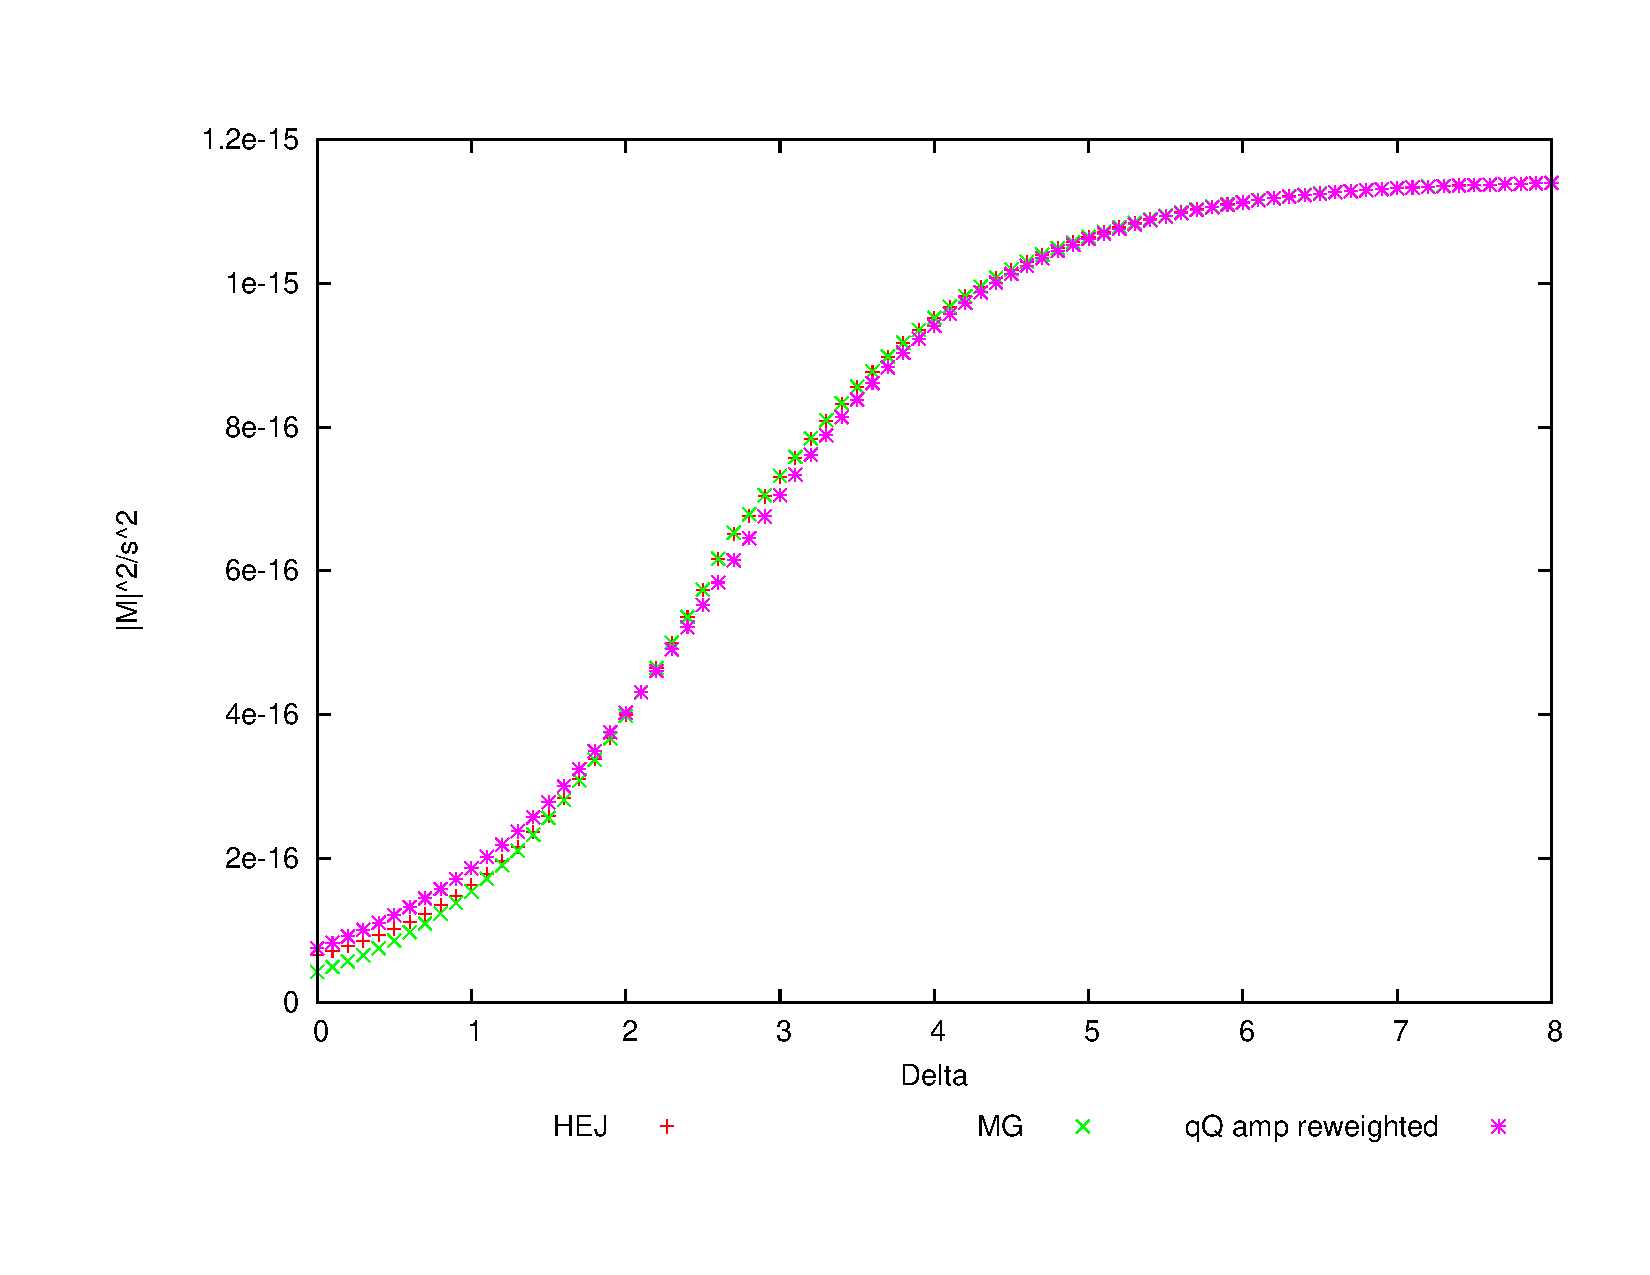
\includegraphics[scale=0.45]{Images/qg_qgH_central.pdf}
\caption{Comparison between the HEJ effective vertex, the full LO result and the result of the $qQ \to qHQ$ LO calculation reweighted by a colour factor for a central $H$ in $gq \to Hgq$ with full top mass dependence.}
\label{fig:gu_ghu_cen}
\end{figure}
%\todo{Pale green on plots hard to see}
Our second phase space parametrisation fixes the Higgs boson to always be close to the gluon in rapidity whilst the two jets move further apart in rapidity. Explicitly 
\begin{subequations}
\begin{align}
p_1 &= (40 \sqrt{2} \cosh(\Delta),-40,40,40 \sqrt{2} \sinh(\Delta)), \\
p_H &= (\sqrt{40^2+m_H^2} \cosh(\Delta+0.5), 0,-40,\sqrt{40^2+m_H^2}  \sinh(\Delta + 0.5)), \\
p_2 &= (40 \cosh(-\Delta),40,0,40 \sinh(-\Delta)).
\end{align}
\end{subequations}
In figure \ref{fig:gu_ghu_out}, we plot this new effective vertex approach against the full LO result with this set of momenta. We also include the result of the reweighted $qQ \to qHQ$ amplitude to show that this is not an appropriate result in this limit. 
\begin{figure}[t]
\centering
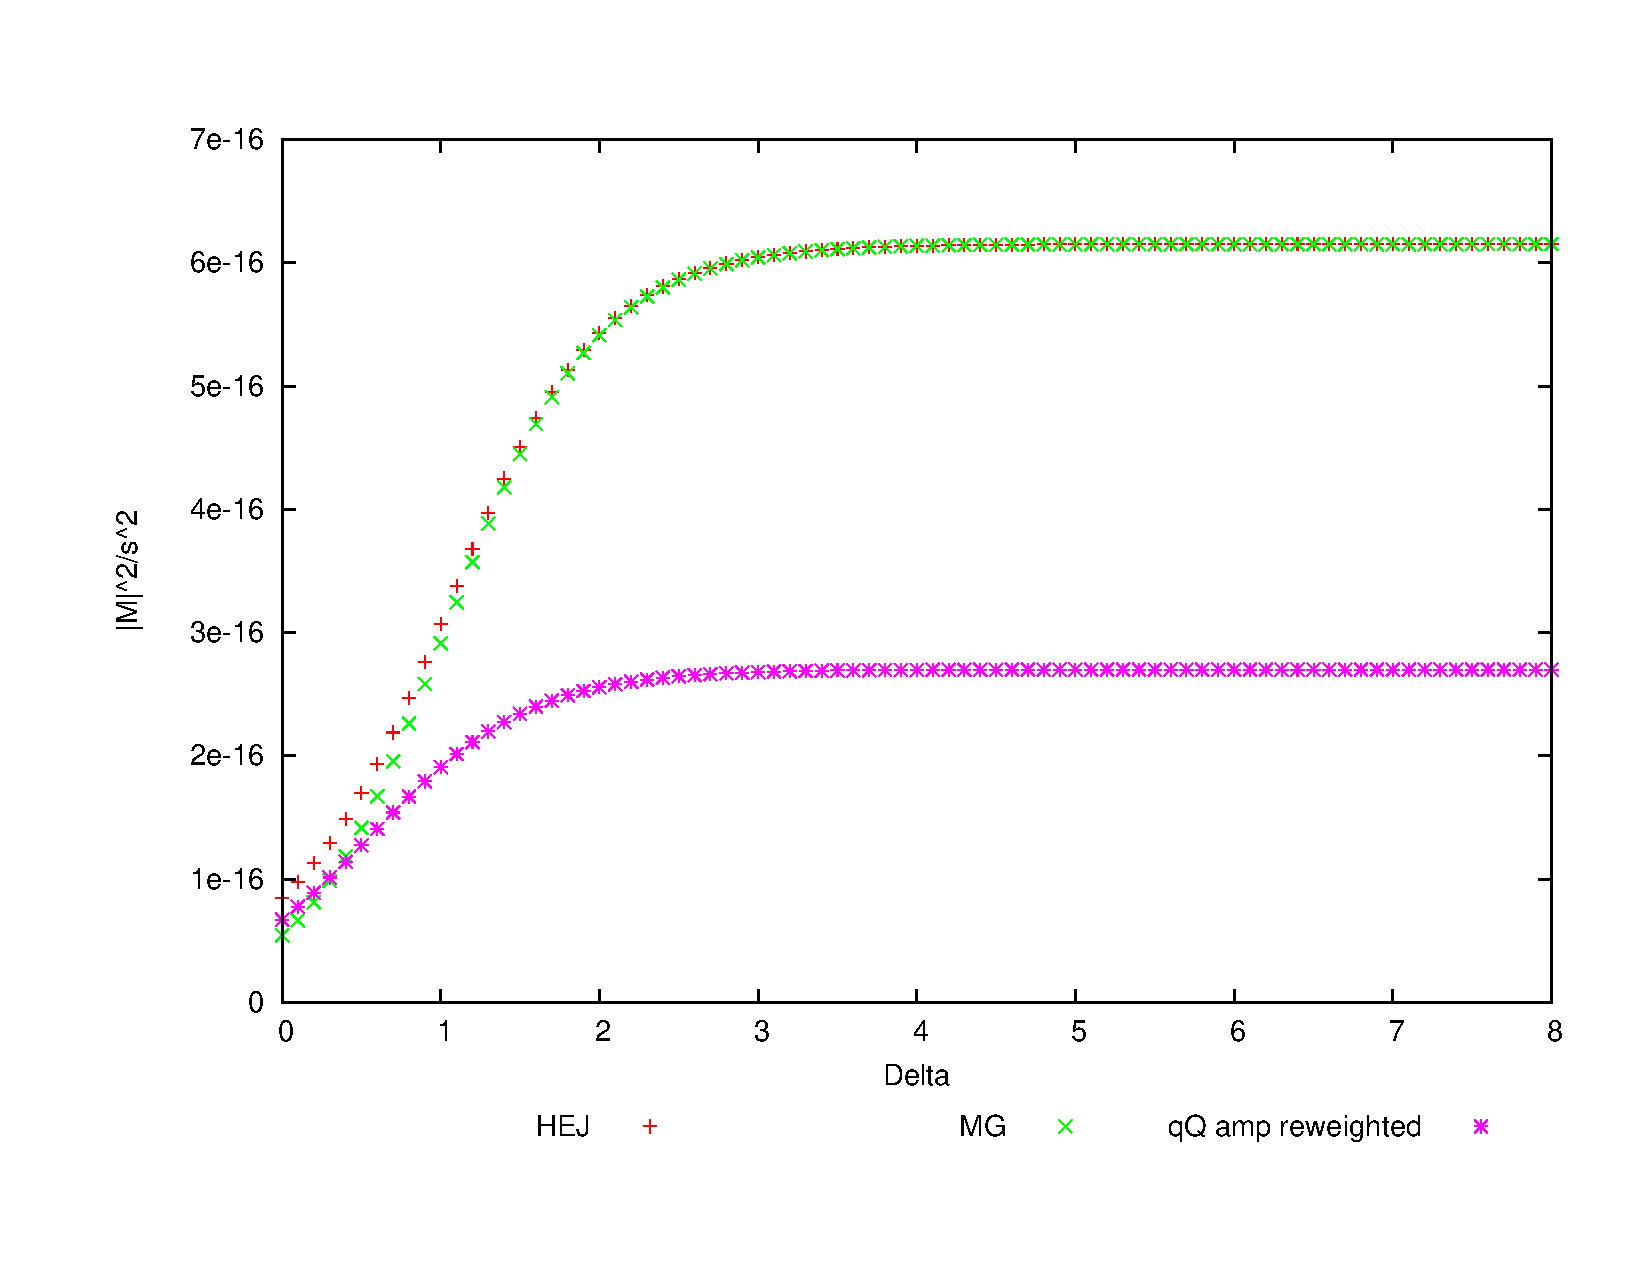
\includegraphics[scale=0.45]{Images/qg_qgH_outside.pdf}
\caption{Comparison between the HEJ effective vertex, the full LO result and the result of the $qQ \to qHQ$ LO calculation reweighted by a colour factor for an outside $H$ in $gq \to Hgq$ with full top mass dependence.}
\label{fig:gu_ghu_out}
\end{figure}
In both cases, we see clear agreement between our result and the full LO result from MadGraph in the High Energy (high $\Delta$) Limit and relatively small deviations below this. We now move on to check the effects of having a finite quark mass as opposed to an infinite one. By simply putting a high value for the top mass in our amplitude (numerically, we see that $m_t = 17400$ is a good choice -- higher values are unstable) we can generate results that correspond to the effective theory where the top mass is treated as an infinite parameter. Additionally, we can very easily add the interference via bottom loops to our result (when working out the amplitudes for helicity configurations, simply add the same amplitude with the bottom mass before squaring it) so we can also see how large an effect this has. We will begin by looking at these three cases with a central Higgs (the first set of momenta), which is plotted in figure \ref{fig:qg_qgh_compare}. We see that there are clear differences between the cases. The finite top mass case is always greater than the infinite top mass case -- in the High Energy Limit, this difference is around 3\%. The addition of the bottom quark increases this difference by a further 3\%. The same comparison for a Higgs close to the gluon (the second set of momenta) is plotted in figure \ref{fig:qg_qgh_compare_out}. In that case, we have slightly different behaviour - the infinite top mass case is still lower (approximately 5\% lower than the finite top mass line), but now the addition of the bottom loop (slightly) decreases the ME from the case where only the top quark is considered. 

\begin{figure}[t]
\centering
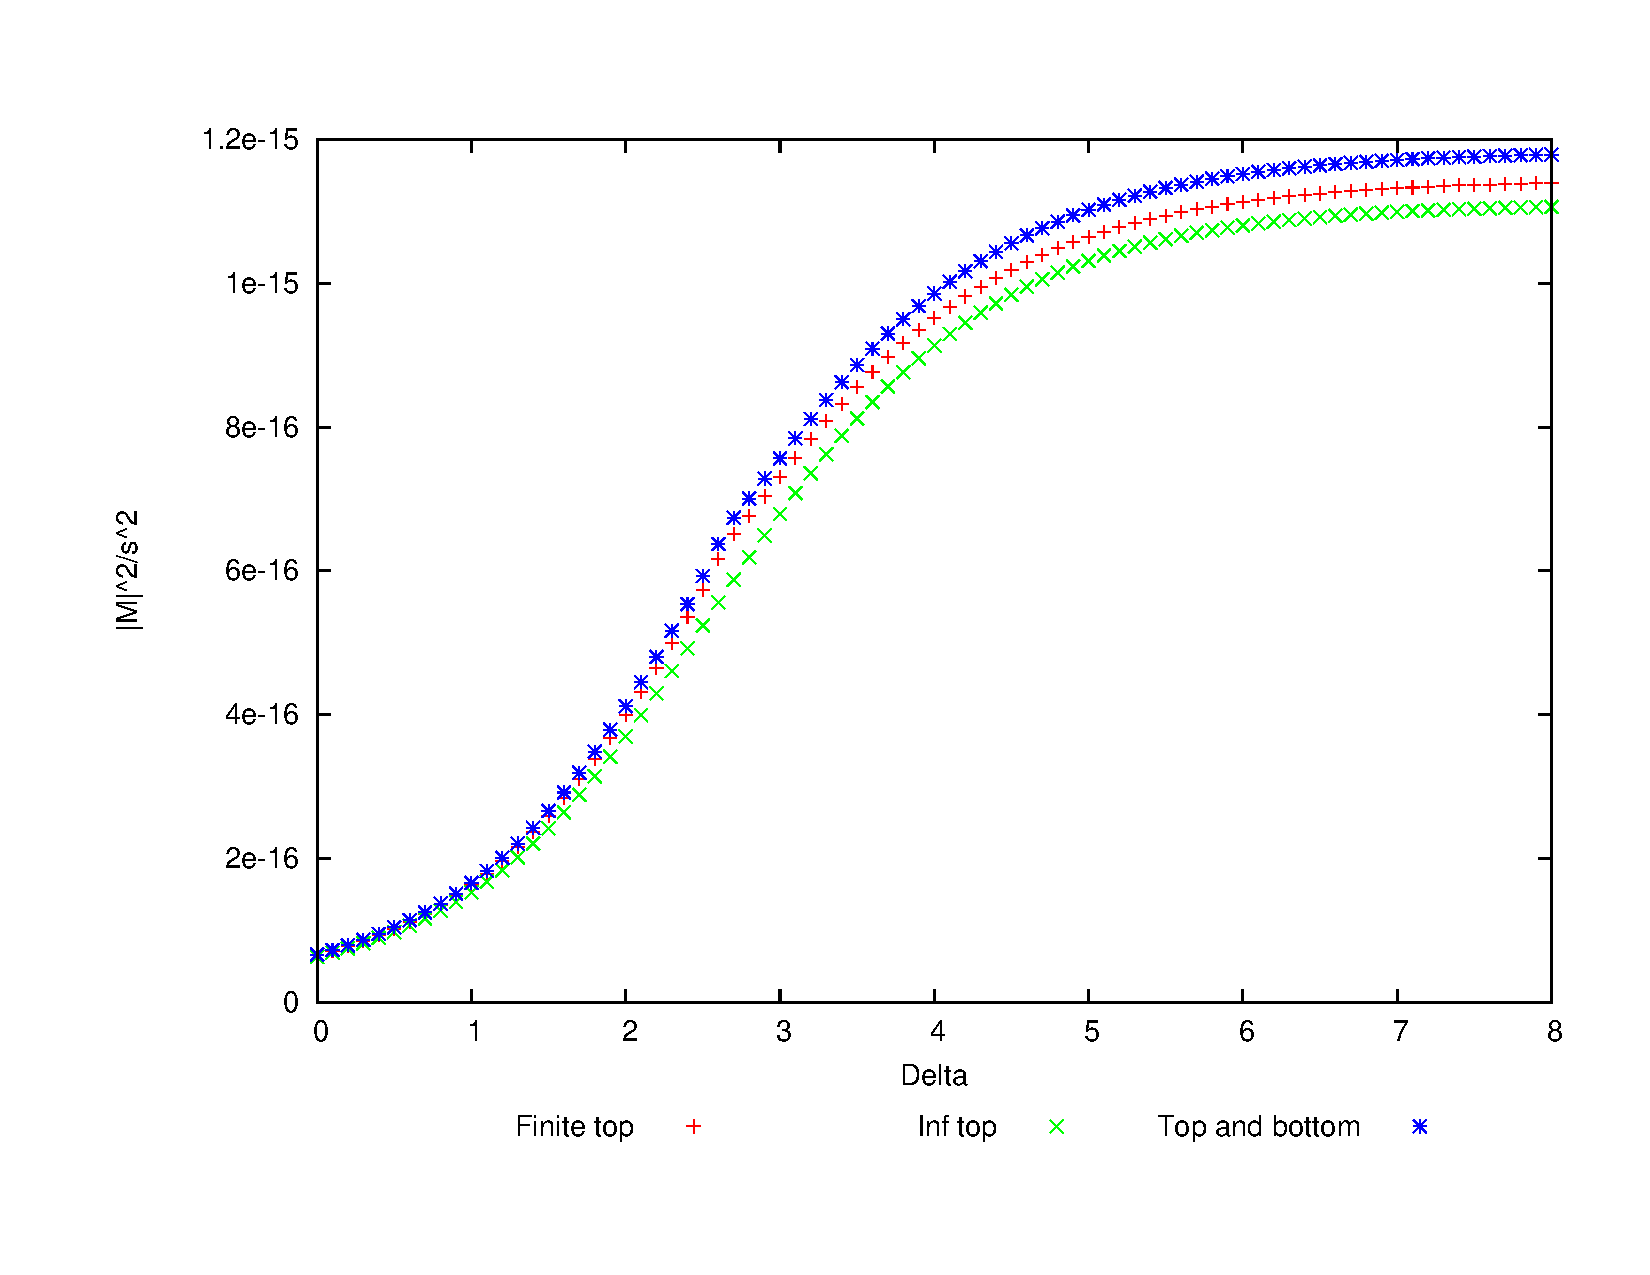
\includegraphics[scale=0.45]{Images/qg_qgH_compare_central.pdf}
\caption{Comparison of infinite top, finite top and finite top plus finite bottom HEJ matrix elements with a central Higgs.}
\label{fig:qg_qgh_compare}
\end{figure}

\begin{figure}[t]
\centering
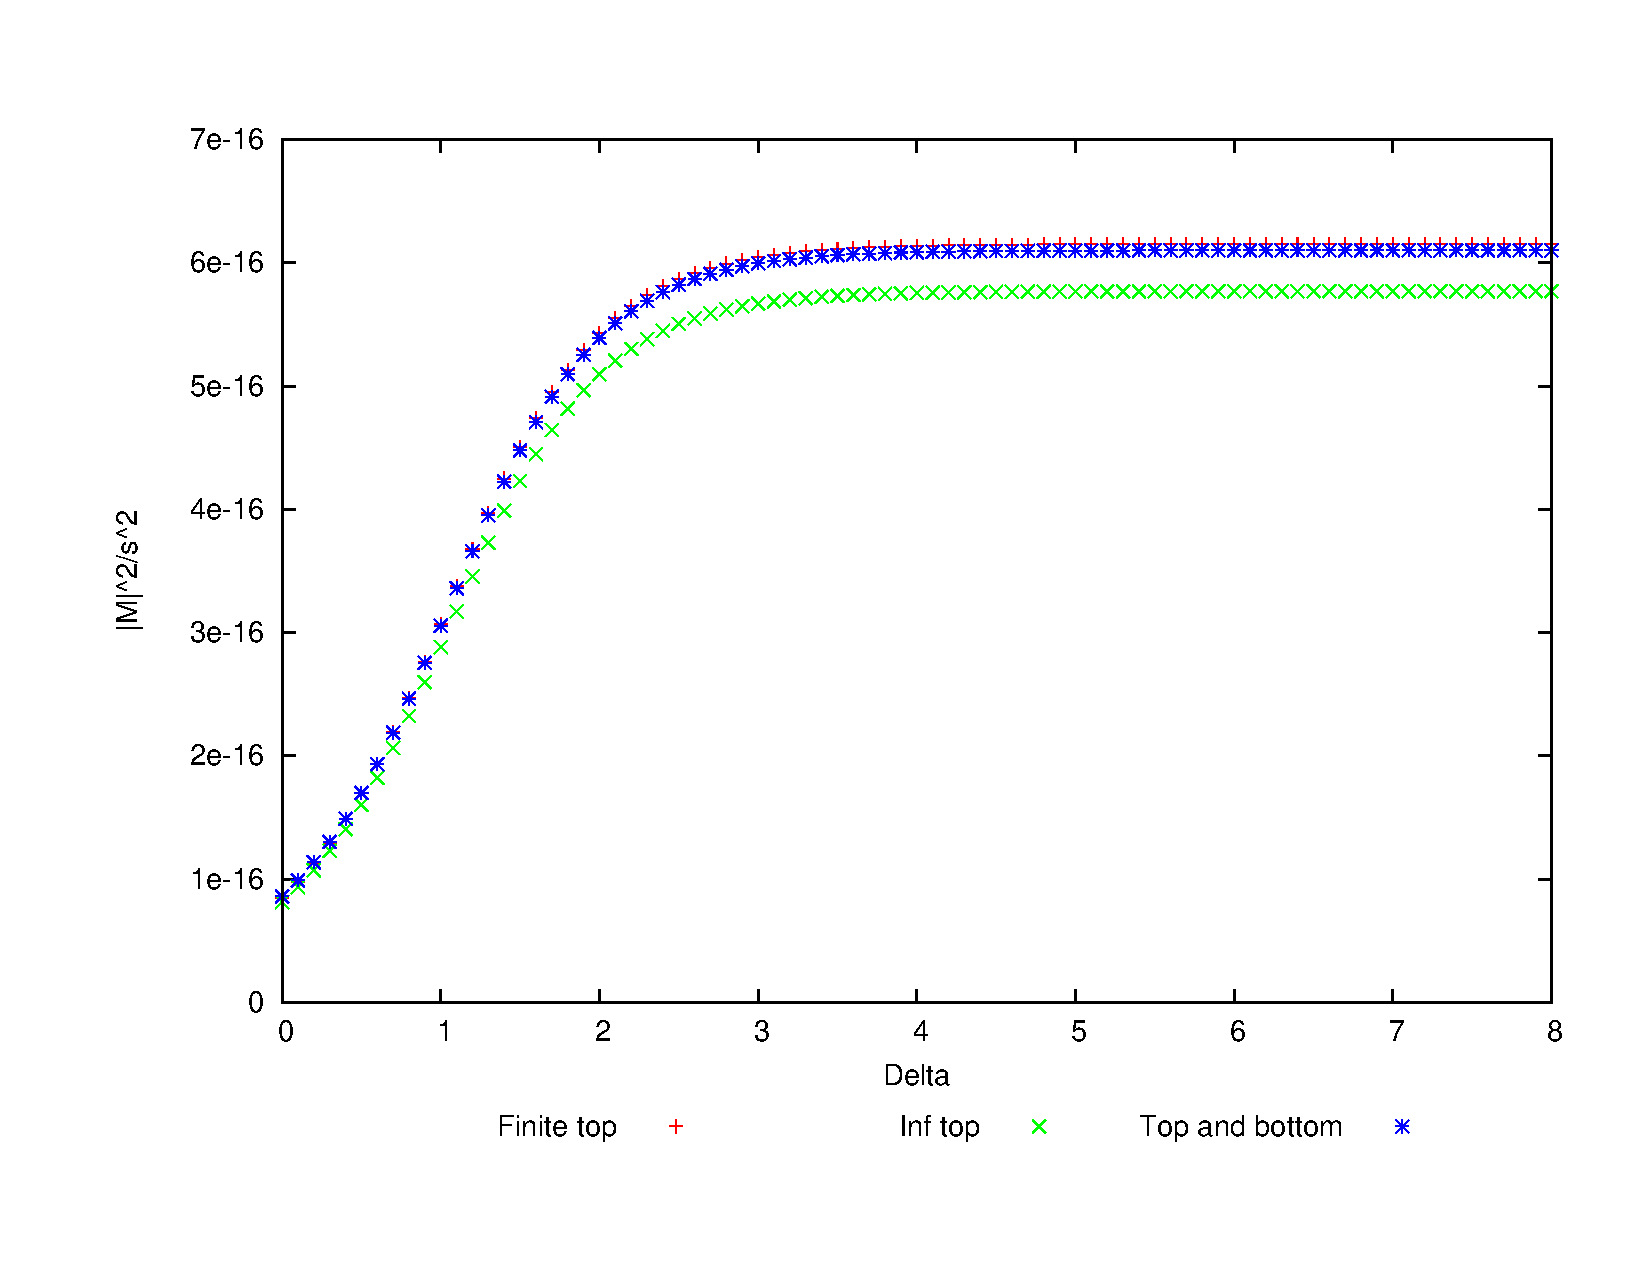
\includegraphics[scale=0.45]{Images/qg_qgH_compare_outside.pdf}
\caption{Comparison of infinite top, finite top and finite top plus finite bottom HEJ matrix elements with an outside Higgs.}
\label{fig:qg_qgh_compare_out}
\end{figure}

The addition of extra emissions is again achieved by multiplying Lipatov vertices into the amplitude we have derived. Some care is required to ensure the correct $t$-channel momenta are taken, resulting in a general $gq\to Hg...q$ amplitude (where the ... represent an arbitrary number of gluons) which is simply
\begin{equation}
|M_{gq \to Hg...q}^{HE,m_t}|^2 = |M_{gq \to Hgq}^{HE,m_t}|^2 \times \prod_{i=1}^{n-2} \frac{-g_s^2C_A V^\mu(q_i, q_{i+1}) V_\mu(q_i, q_{i+1})}{q_i^2},
\end{equation}
where $n$ is the number of final state jets and the $q_i$ are the $t$-channel momenta entering the Lipatov vertices -- we define $q_1 = p_a - p_1 -p_H$ and $q_i = q_{i-1} - p_i$ for $i >1$. As a check, we will generate more explorer plots for the case of one extra emission. We will choose the process $gu \to Hggu$ with a few different choices for the rapidity of the extra gluon and the Higgs to ensure we are calculating correctly. Our first configuration is used for when the Higgs is being emitted close to the extremal gluon
\begin{subequations}
\begin{align}
p_1 &= (40 \cosh(\Delta),-40,0,40 \sinh(\Delta)), \\
p_H &= (\sqrt{40^2+m_H^2} \cosh(\Delta+0.5), 0,-40,\sqrt{40^2+m_H^2}  \sinh(\Delta+0.5)), \\
p_2 &= (40 \cosh(-\Delta/3),0,40,0), \\
p_3 &= (40 \cosh(-\Delta),40,0,40 \sinh(-\Delta)).
\end{align}
\end{subequations}
We show $|M|^2/\hat{s}^2$ as a function of $\Delta$ in figure \ref{fig:ug_for} for this configuration. Because the finite $m_t$ result available in MadGraph is numerically unstable at high $\Delta$, we will instead set $m_t$ to $17400$ and compare to the full LO effective theory matrix element, available in earlier versions of MadGraph. \todo{could actually show this in a plot}

\begin{figure}[t]
\centering
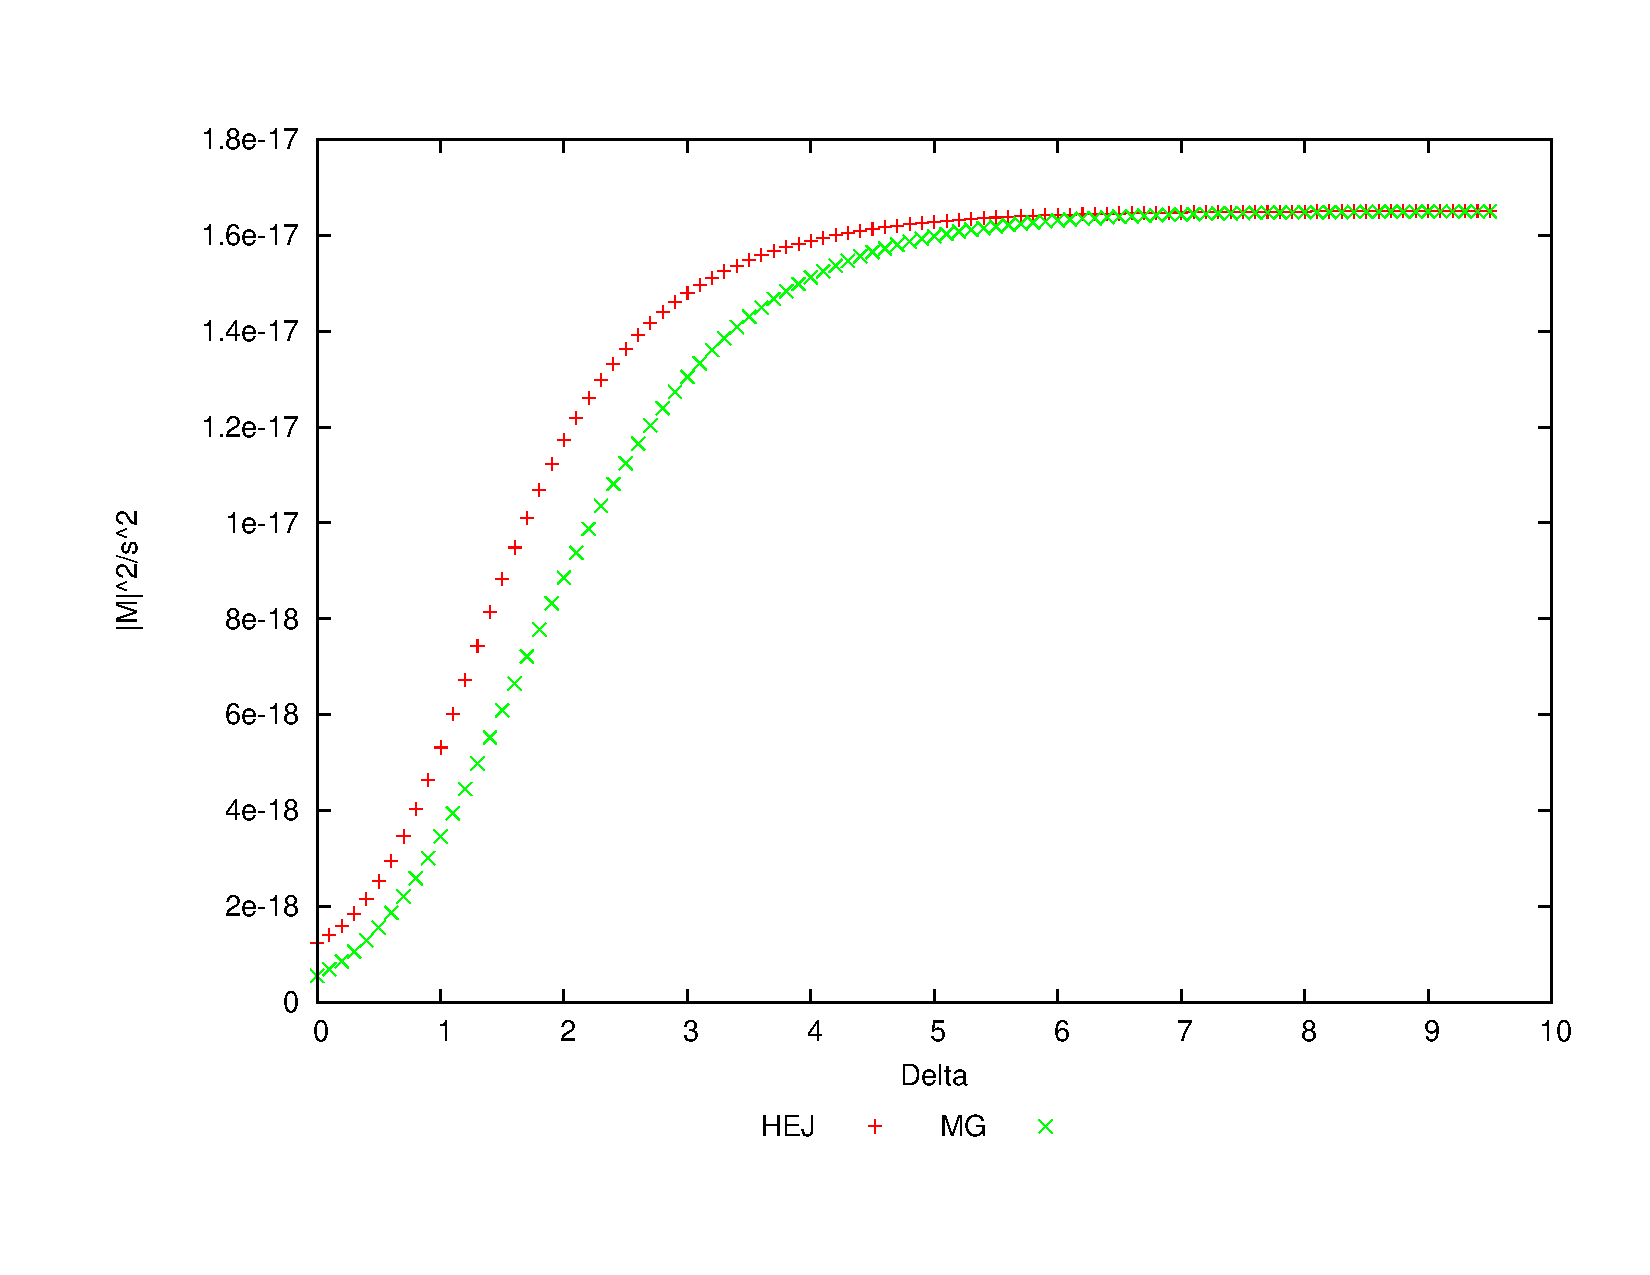
\includegraphics[scale=0.45]{Images/ug_nextfor.pdf}
\caption{Comparison between the HEJ effective vertex and the full LO result of the $gu \to Hggu$ amplitude for a forward $H$ with an infinite top mass.}
\label{fig:ug_for} 
\end{figure}
%\todo{Swear this looked better before? Regenerate}

The agreement here is good across the phase space and almost identical above $\Delta = 6$. Another slice of phase space we can take is one where all particles gradually move apart in rapidity:
\begin{subequations}
\begin{align}
p_1 &= (40 \cosh(\Delta),-40,0,40 \sinh(\Delta)), \\
p_H &= (\sqrt{40^2+m_H^2} \cosh(\Delta/3), 0,-40,\sqrt{40^2+m_H^2}  \sinh(\Delta/3)), \\
p_2 &= (40 \cosh(-\Delta/3),0,40,40 \sinh(-\Delta/3)), \\
p_3 &= (40 \cosh(-\Delta),40,0,40 \sinh(-\Delta)).
\end{align}
\end{subequations}
\begin{figure}[t]
\centering
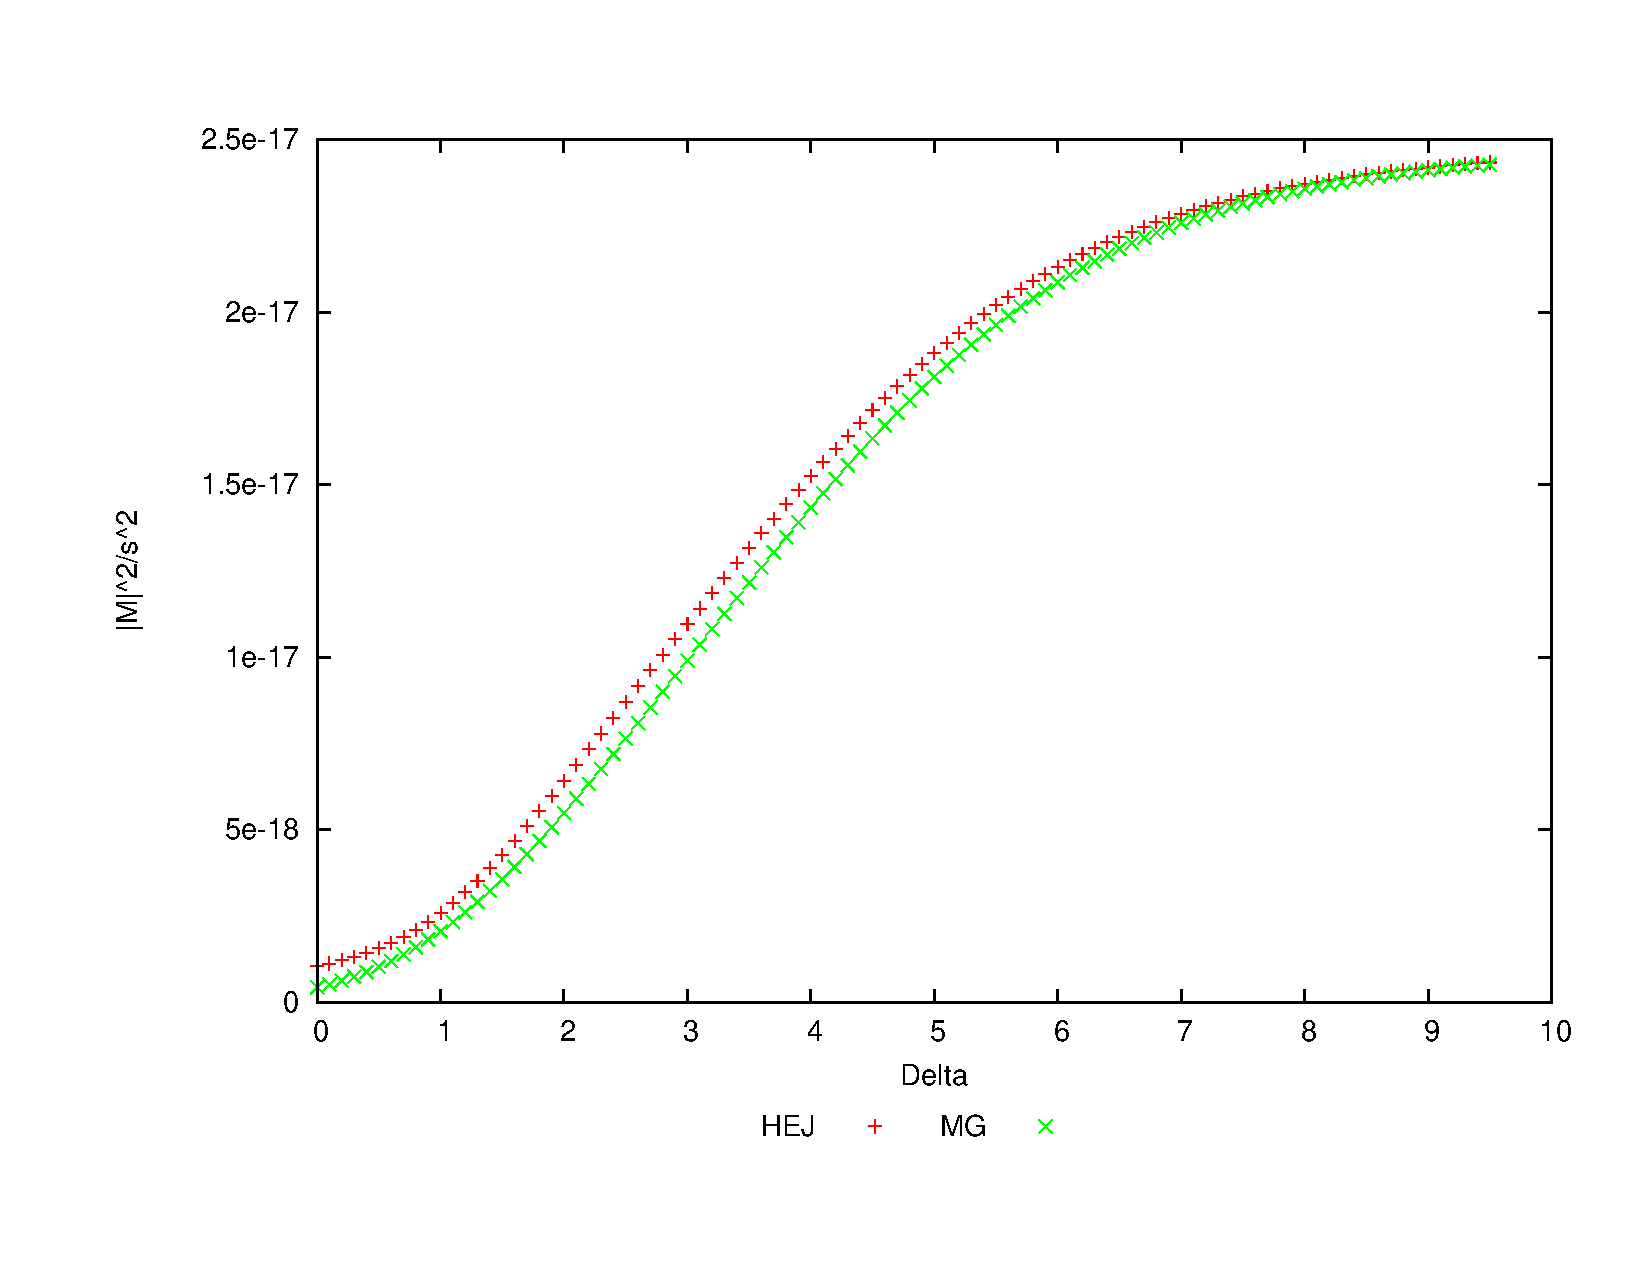
\includegraphics[scale=0.45]{Images/ug_cen.pdf}
\caption{Comparison between the HEJ effective vertex and the full LO result of the $gu \to gHgu$ amplitude for a central $H$ with an infinite top mass.}
\label{fig:ug_cen}
\end{figure}

The explorer plot for this configuration is shown in figure \ref{fig:ug_cen}. Again, the agreement is good between the two lines across the full range. The other configuration to check is the one where the Higgs boson is more behind the extra emission. This contribution cannot be described by this matrix element for the $gq$ incoming state, but it can describe the process with the $gg$ incoming state.  In that case, we can send $p_z \to -p_z$ in $p_2$ and $p_H$ in our momenta sets to probe this contribution. In figures \ref{fig:gg_ggh_1}, \ref{fig:gg_ggh_2}, \ref{fig:gg_ggh_3} and \ref{fig:gg_ggh_4}, we show $gg \to Hggg$ with the Higgs being more forward, central but more forward than the extra emission, central but more backward than the extra emission and more backward respectively. All plots show agreement in the large $\Delta$ region, as expected, and track the LO result fairly well over the entire range. For small values of $\Delta$, the deviation of our result from the full LO result is quite pronounced. This is typical of the $gg$ incoming state for all HEJ matrix elements \cite{Andersen2009a} since there are contributions from diagrams that are strongly suppressed in the high $\Delta$ limit (and therefore dropped in the derivation of our amplitudes) but are quite important at low $\Delta$. Confident in our forms for the matrix elements, we can move on to implementing them within the HEJ program and investigating their behaviour over the whole range of integrated phase space.

\begin{figure}[t]
\centering
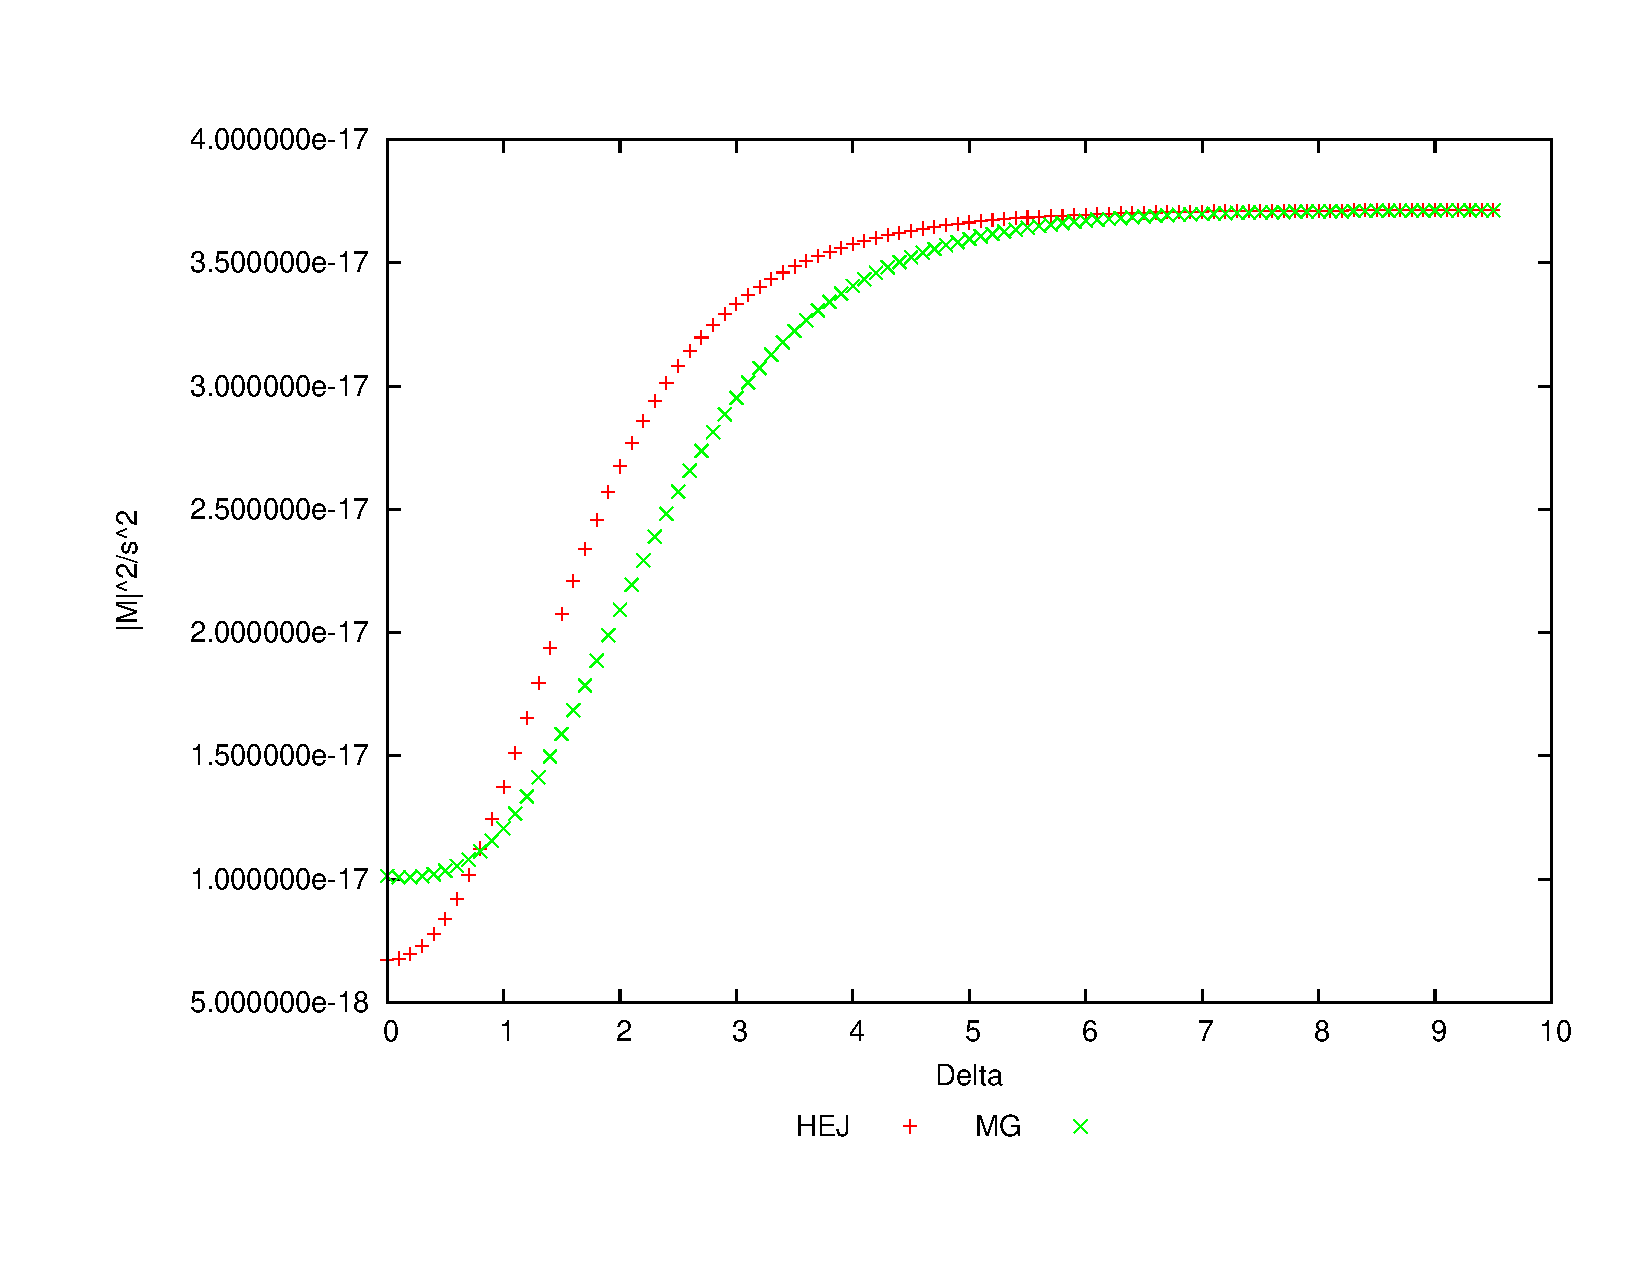
\includegraphics[scale=0.45]{Images/gg_nextfor.pdf}
\caption{Comparison between the HEJ effective vertex and the full LO result of the $gg \to Hggg$ amplitude for a forward $H$ with an infinite top mass.}
\label{fig:gg_ggh_1}
\end{figure}

\begin{figure}[t]
\centering
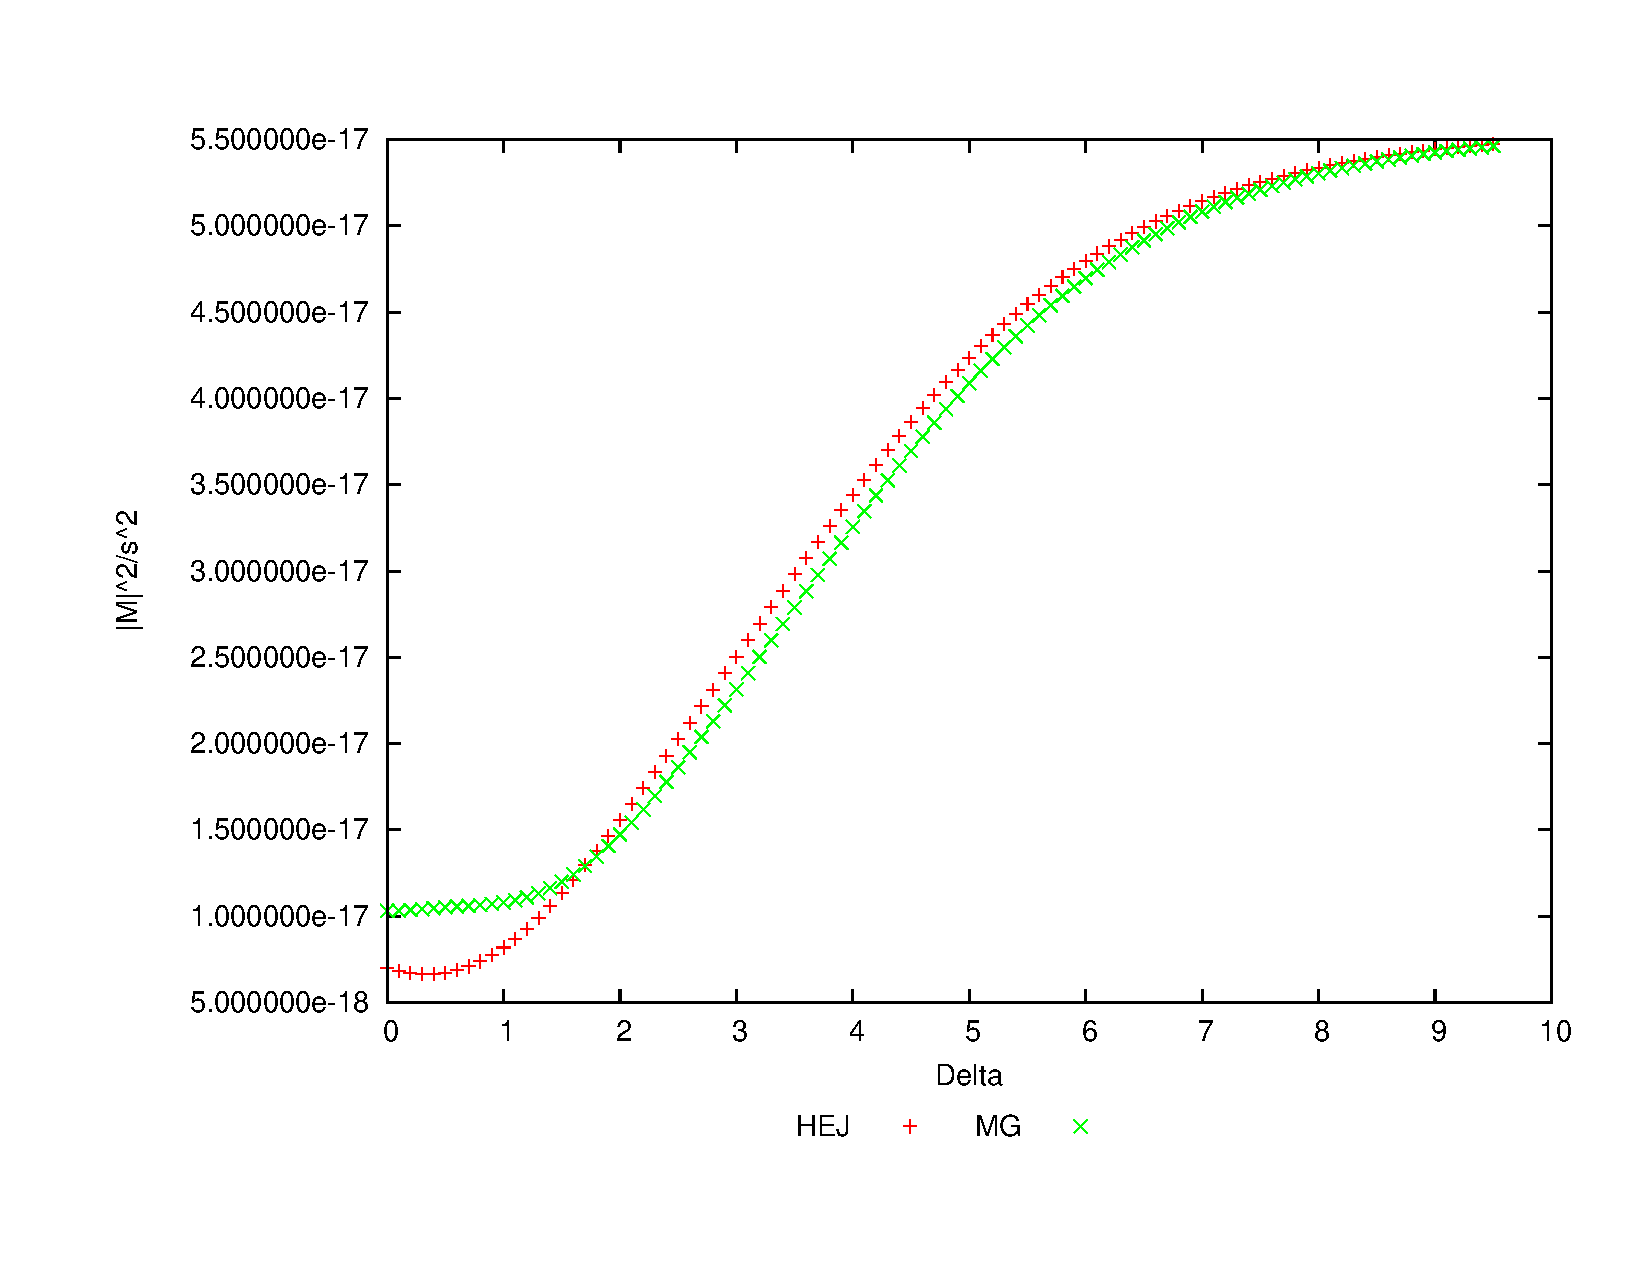
\includegraphics[scale=0.45]{Images/gg_cen1.pdf}
\caption{Comparison between the HEJ effective vertex and the full LO result of the $gg \to gHgg$ amplitude for a central $H$ next to the extremal forward parton with an infinite top mass.}
\label{fig:gg_ggh_2}
\end{figure}

\begin{figure}[t]
\centering
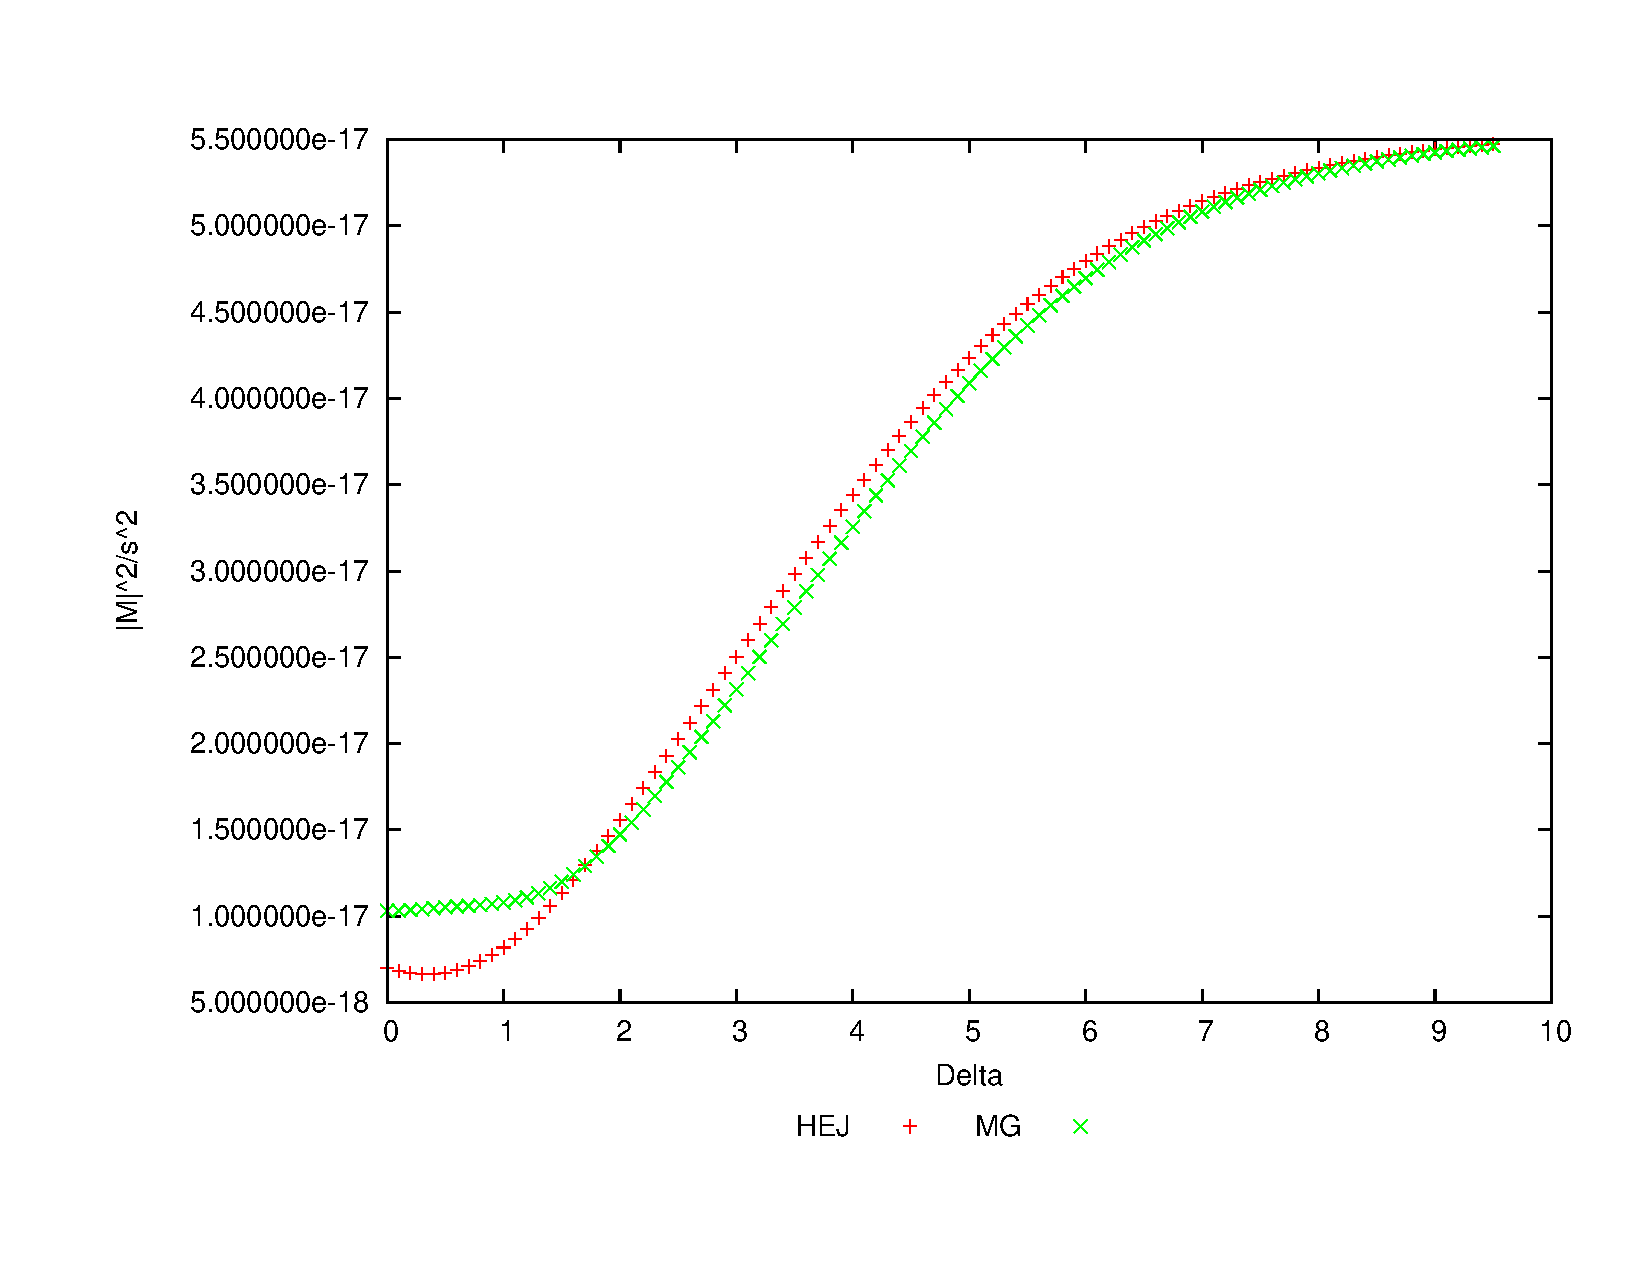
\includegraphics[scale=0.45]{Images/gg_cen2.pdf}
\caption{Comparison between the HEJ effective vertex and the full LO result of the $gg \to ggHg$ amplitude for a central $H$ next to the extremal backward parton with an infinite top mass.}
\label{fig:gg_ggh_3}
\end{figure}


\begin{figure}[t]
\centering
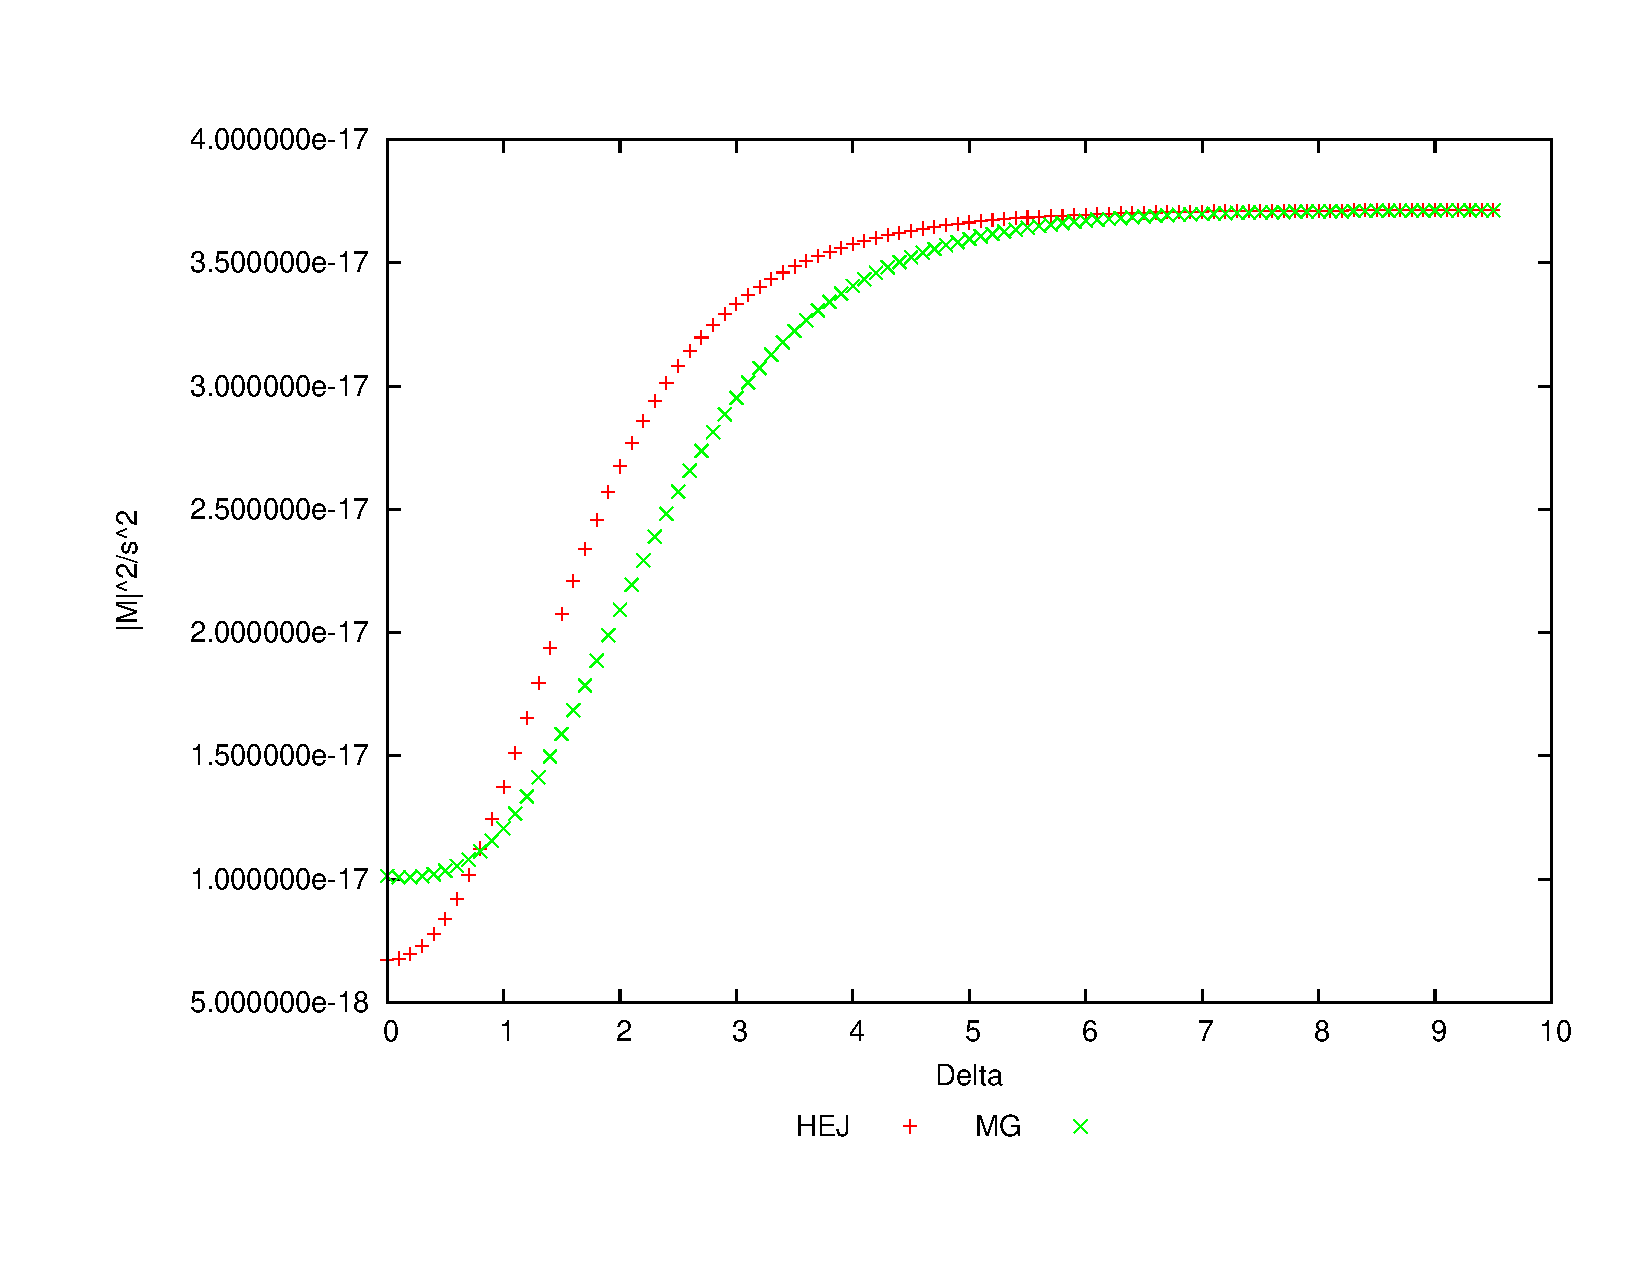
\includegraphics[scale=0.45]{Images/gg_nextback.pdf}
\caption{Comparison between the HEJ effective vertex and the full LO result of the $gg \to gggH$ amplitude for a backward $H$ with an infinite top mass.}
\label{fig:gg_ggh_4}
\end{figure}

\clearpage

\section{Final Exentions and the All-Order Amplitude}
We are almost ready to present a form for the all-order amplitude. Before we do, we first must revisit one point we made earlier: that the analytical form of the matrix element written here assumed that the gluon was the forward-moving particle. In any real analysis, we will have the situation where the gluon is travelling either backwards or forwards and the mathematical difference is the multiplication of a phase factor in some of the amplitude's terms. There is clearly a symmetry between the two cases and so any integration over phase space should yield the result that the contribution from this process with a forward-moving gluon should equal the contribution from the same process with a backward-moving gluon. We will show this to be the case in the next section. 

With that taken into account, we are ready to discuss the all-order expression. As with all other HEJ amplitudes, the generalisation to all orders is simple. In the previous section, we derived an expression for the $gq \to Hgq$ amplitude in a $t$-channel factorised form and then showed how extra gluon emissions are taken into account. The all-order resummation is once more performed by making the following replacement for all $t$-channel gluon propagators:
\begin{equation}
\frac{1}{\hat{t}_i} \to \frac{1}{\hat{t}_i} \exp \left[ \omega_0(q_{i\perp})(y_{i+1} - y_i) \right],
\end{equation}
where $\omega(q_i)$ is defined in equation \ref{eqn:omega}. 

This gives the form of the all-order amplitude to be (where we emphasise that the rapidity ordering can be either backwards-to-forwards or forwards-to-backwards with the correct phase multiplication of terms in the base amplitude)
\begin{equation}
\begin{split}
|M_{gf_2 \to Hg...f_2}^{HEJ,m_t}|^2 &= \frac{1}{4(N_C^2-1)}|M_{gq \to Hgq}^{HE, m_t}|^2 \cdot \frac{C_{f_2}}{C_F} \\
&\cdot \prod_{i=1}^{n-2} \frac{-g^2 C_A V(q_{i}, q_{i+1}) \cdot V(q_{i}, q_{i+1})}{\hat{t}_{i} \hat{t}_{i+1}}  \\
& \cdot\prod_{j =1}^{n-1} \exp \left[ \omega_0(q_{j \perp})(y_{j+1} - y_j) \right],
\end{split}
\end{equation}
where $C_{f_2} = \tilde{C}_A$ if $f_2$ is a gluon or $C_F$ if it is a quark and the notation `$...$' signifies the emission of $n-2$ gluons with $n$ being the total number of colour-charged particles in the final state. We define $q_1 = p_a - p_1 -p_H$ and $q_i = q_{i-1} - p_i$ after that and remind ourselves that there is already a division by $\hat{t}_1 \hat{t}_{n-1}$ defined within the base amplitude, so that the powers and numbers of $t$-channel propagators in this equation is correct. 

In the next section, we describe the considerations needed when incorporating this amplitude in the HEJ program. 

\section{Computational Aspects}

The addition of this new amplitude into the HEJ program is a much simpler task than it was for the NLL processes. Since we already have the amplitude in terms of the impact factors for the infinite top mass cases, the implementation is a case of adding the option to run with this finite top mass element instead. However, in order to calculate the scalar integrals in this amplitude, a HEJ interface to LoopTools is required. This is achieved in the program by setting a special instruction in the makefile; this way, if a user is not interested in using HEJ to generate for these types of events, they do not need LoopTools on their system. On the other hand, with the setting of a few library paths and setting the value for the special flag, LoopTools is quickly and simply added to the program such that running these new amplitudes can be performed `out of the box'. 

Another consideration is how to implement the matching for the finite top mass case. Given the length of time it would take to evaluate the matrix element with the full top mass included (especially in the three jet case), it would not be feasible for realistic analyses. Instead, since the infinite top mass elements are much quicker to evaluate, the matching is implemented by applying the infinite top mass limit to the HEJ amplitude and dividing that by the full LO result in the effective theory. This yields an acceptable compromise as the correction of the Born approximation should be independent of the $m_t$ effects, but it would clearly be ideal to match to the full result if the amount of time needed to do so was significantly reduced. This latter point is one motivation behind the development of the `inverse HEJ' technique. Since there are many resummation processes that can map to one jet process, the idea is to instead generate the jet level matrix element and work backwards from that to generate many resummation points to evaluate: hence, `inverse'. This will drastically reduce the amount of calls made to the full finite top mass LO matrix element and thus allow us to include this matching. 
%\todo{Make this a bit meatier. Include matching only to inf. Inverse HEJ?}

\section{Results}
%\todo{Explorer plots, integrated plots, other interesting things to note. Last real section to do! Arggh!}

Our first integrated distributions will be for the $gu \to gu + H$ process, where we restrict ourselves to the case where the gluon is the forward-moving particle and the $u$ quark is the backward-moving particle. The Higgs can then be more forward than the gluon ($Hgu$), more backward than the quark ($guH$) or in between the two particles in rapidity ($gHu$). For the forward case, we will use the matrix element derived in section 4.2 to describe the process. For the central case, we will use the reweighted $qQ$ amplitude from section 4.1. Although our new matrix element will get this case correct, the reason we do not use it here is in anticipation of our resummation technique. Because we resum $t$-channel gluons, it is important to have a system where we can always unambiguously define what those gluons will be (or, in other words, we must have a consistent `resummation region', which for us will be the rapidity space between the gluon and quark). With our new amplitude, we can only resum the gluon connecting the effective vertex to the quark line, but for the reweighted $qQ$ case, we can resum the gluon from the top quark line to the triangle loop in the middle of the diagram and then from the triangle loop down to the bottom quark line. Choosing which matrix element we use based on the rapidity of the Higgs makes it clear which resummation we will be doing. Finally, since we have not discussed the case where the Higgs is behind the outgoing quark, we will set this process to zero for the time being (though in the full HEJ program, this is of course properly incorporated with the appropriate impact factor). %\todo{jenni question - why set to zero?}

An interesting plot to look at is the Higgs $p_T$ spectrum. The infinite top mass limit should not do well at high values of Higgs $p_T$, as discussed in \cite{Duca2003}, because it breaks the idea of the top quark mass being the largest relevant scale. This distribution is shown in figure \ref{fig:higgs_pt}. We see the expected behaviour: at large Higgs $p_T$, the results obtained with the effective theory and the theory with finite quark mass effects are very different. The difference when also including a bottom quark is minimal, leading to slight difference in the low $p_T$ bins which is not large enough to show up on the logarithmic plot. 

Another interesting distribution to look at is the rapidity difference between the gluon and the quark. One could expect that the presence of a large rapidity gap (and so a large dijet invariant mass) might break the infinite top mass limit, but \cite{Duca2003} showed this not to be the case. The distribution shown in figure \ref{fig:higgs_ydiff} also shows little difference and hence agrees with their conclusion. The difference when including a bottom quark is clearer in this distribution, where we see a slight (but definite) drop of the cross-section in the low $\Delta y$ bins. For this analysis, the integrated cross-section is smaller by about 2\% because of this inclusion. 

\begin{figure}[t]
\centering
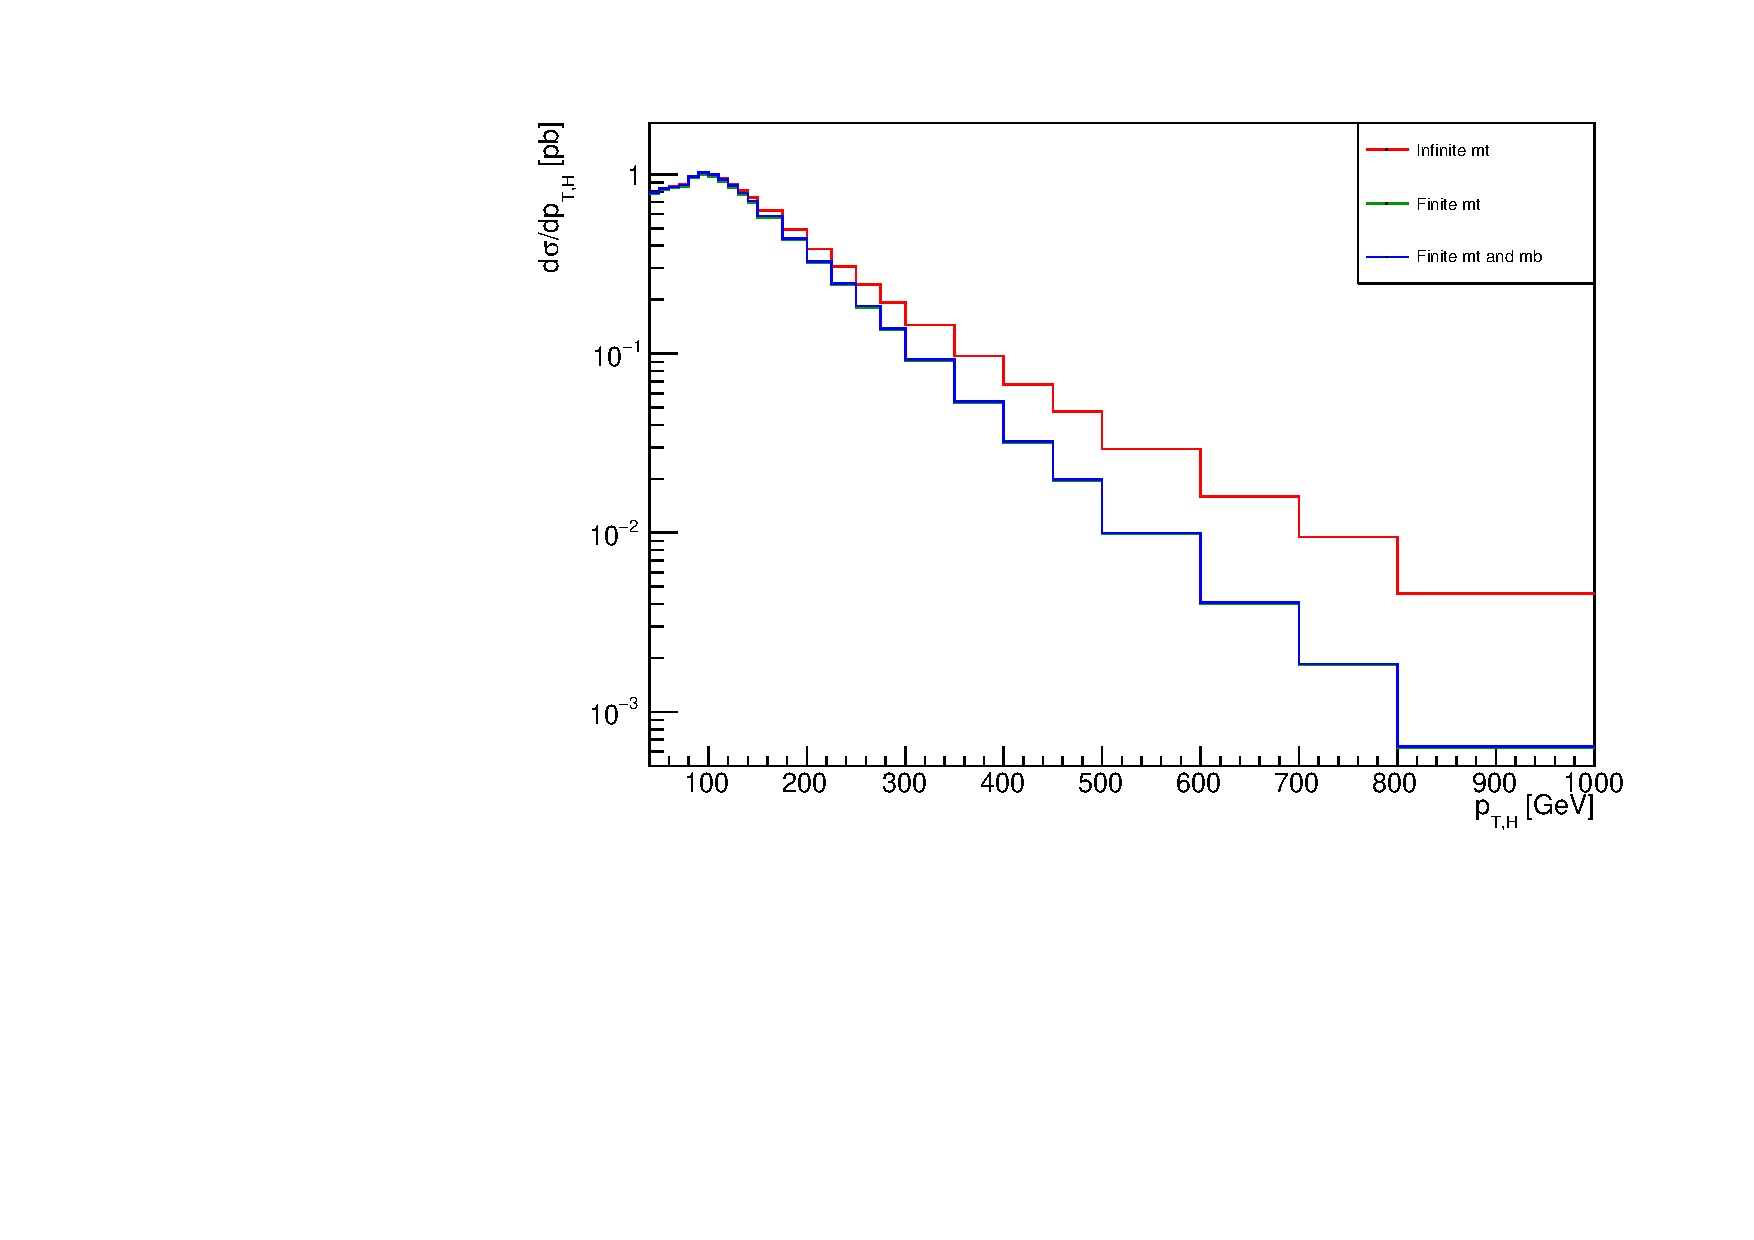
\includegraphics[scale=0.75]{Images/ptH_gu.pdf}
\caption{Comparison of infinite top mass, finite top mass and finite top plus finite bottom mass cross-sections in $gu \to guH$, binned in Higgs $p_T$ }
\label{fig:higgs_pt}
\end{figure}

\begin{figure}[t]
\centering
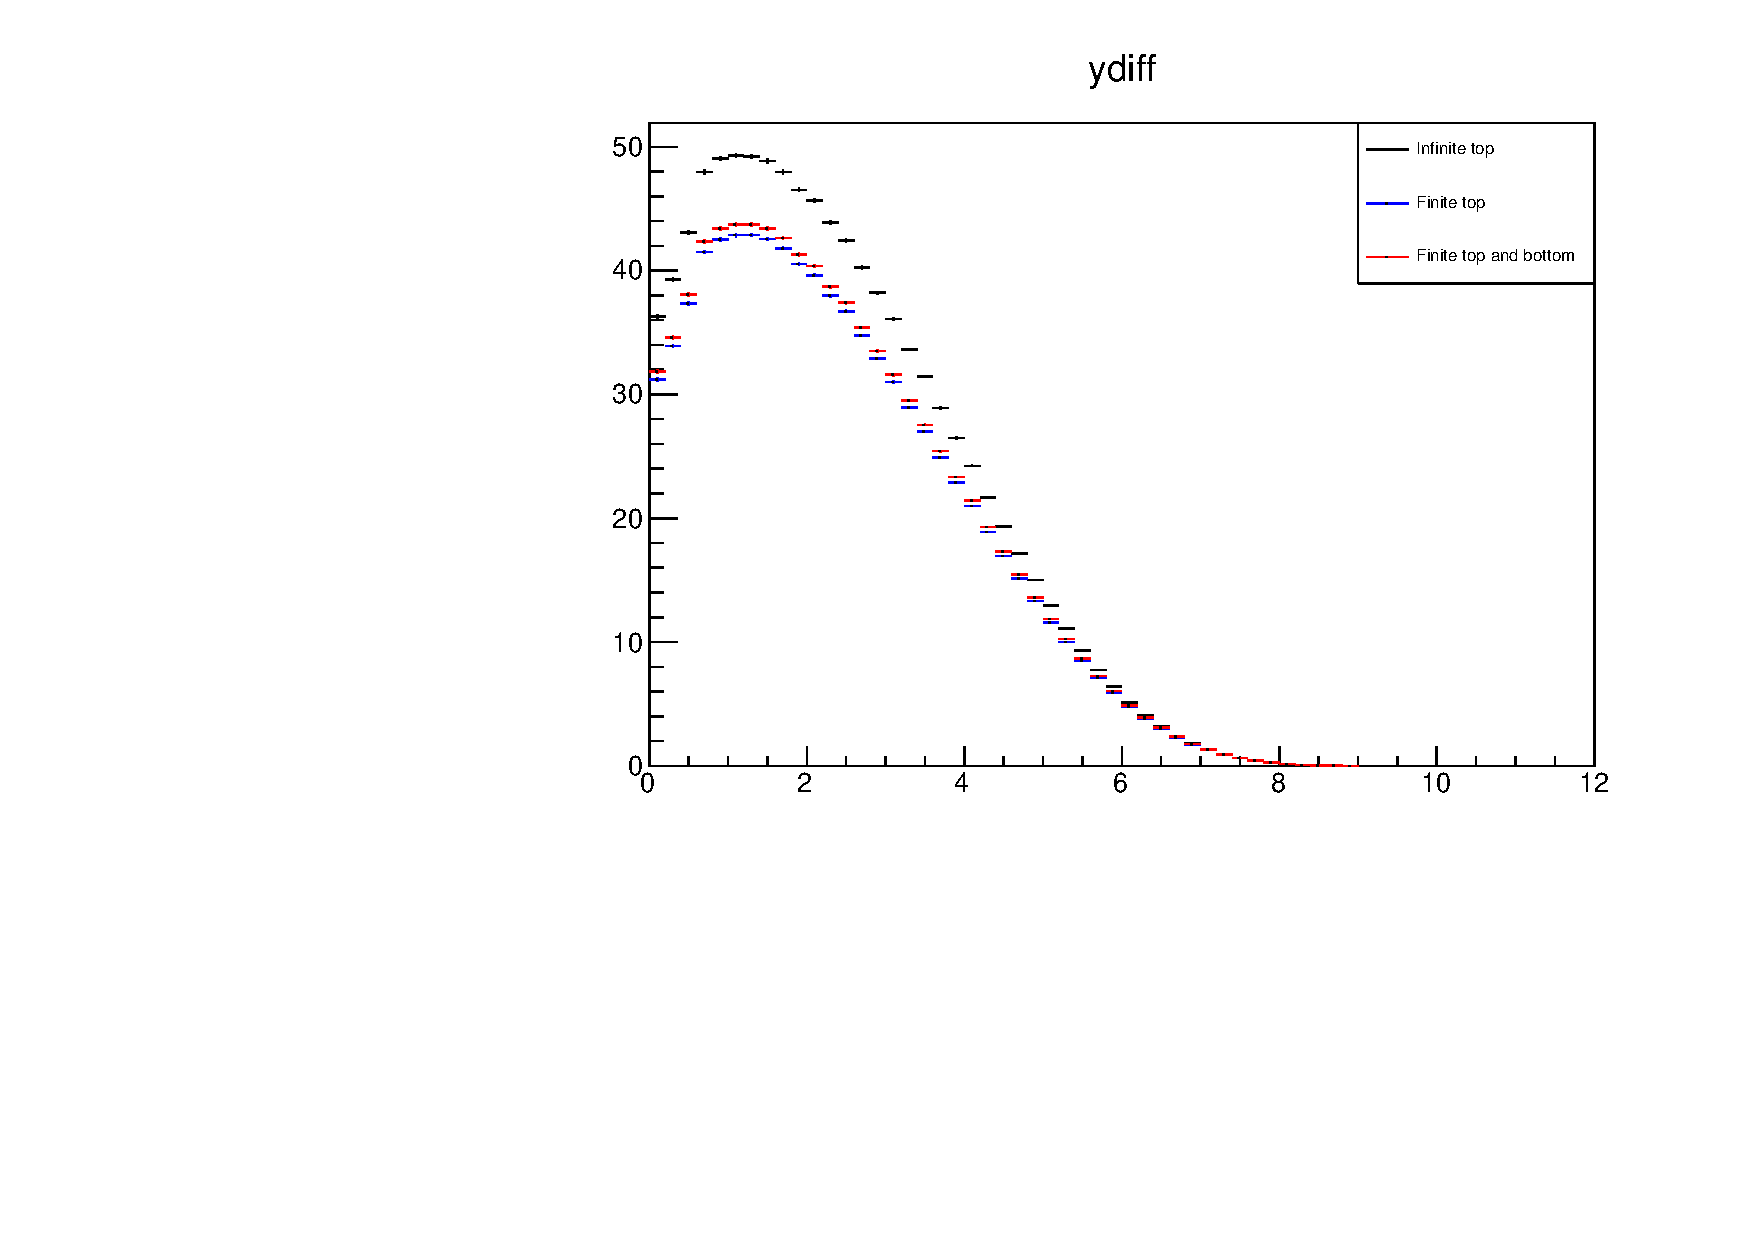
\includegraphics[scale=0.75]{Images/ydiff_gu.pdf}
\caption{Comparison of infinite top mass, finite top mass and finite top plus finite bottom mass cross-sections in $gu \to guH$, binned in rapidity difference between the gluon and up quark}
\label{fig:higgs_ydiff}
\end{figure}

We should also remember that, given kinematical constraints on the energy of the collider, the high $\Delta y$ region must come with relatively low transverse scales, so it further lends support to the idea that the transverse scales are the defining ones in terms of how accurate the effective theory is. We can do the same analysis with a $gg$ incoming state, which in the high energy regime is just the $qg$ amplitude reweighted by a colour factor. In this case, the Higgs can be either forward of a forward-moving gluon, backward of a backward-moving one or in-between. We can describe all of these configurations: the first and second with our new amplitude and the latter with a reweighted $qQ$ amplitude. 

As mentioned in section 4.3, we must have that the cross-section contribution from the forward-moving gluon is equal to the contribution from the backward-moving gluon. We show that this is the case in figure \ref{fig:gg_crosssection}, where the green and blue lines are so close together as to be essentially indistinguishable. The results for the Higgs $p_T$ and $\Delta y_{12}$ distributions are extremely similar to the $gq$ case and we present them here for completeness in figures \ref{fig:pth_gg} and \ref{fig:ydiff_gg}. The most obvious difference is that the $\Delta y$ distribution peaks more to the left of the plot -- an effect of the gluon parton distribution function. 

\begin{figure}[t]
\centering
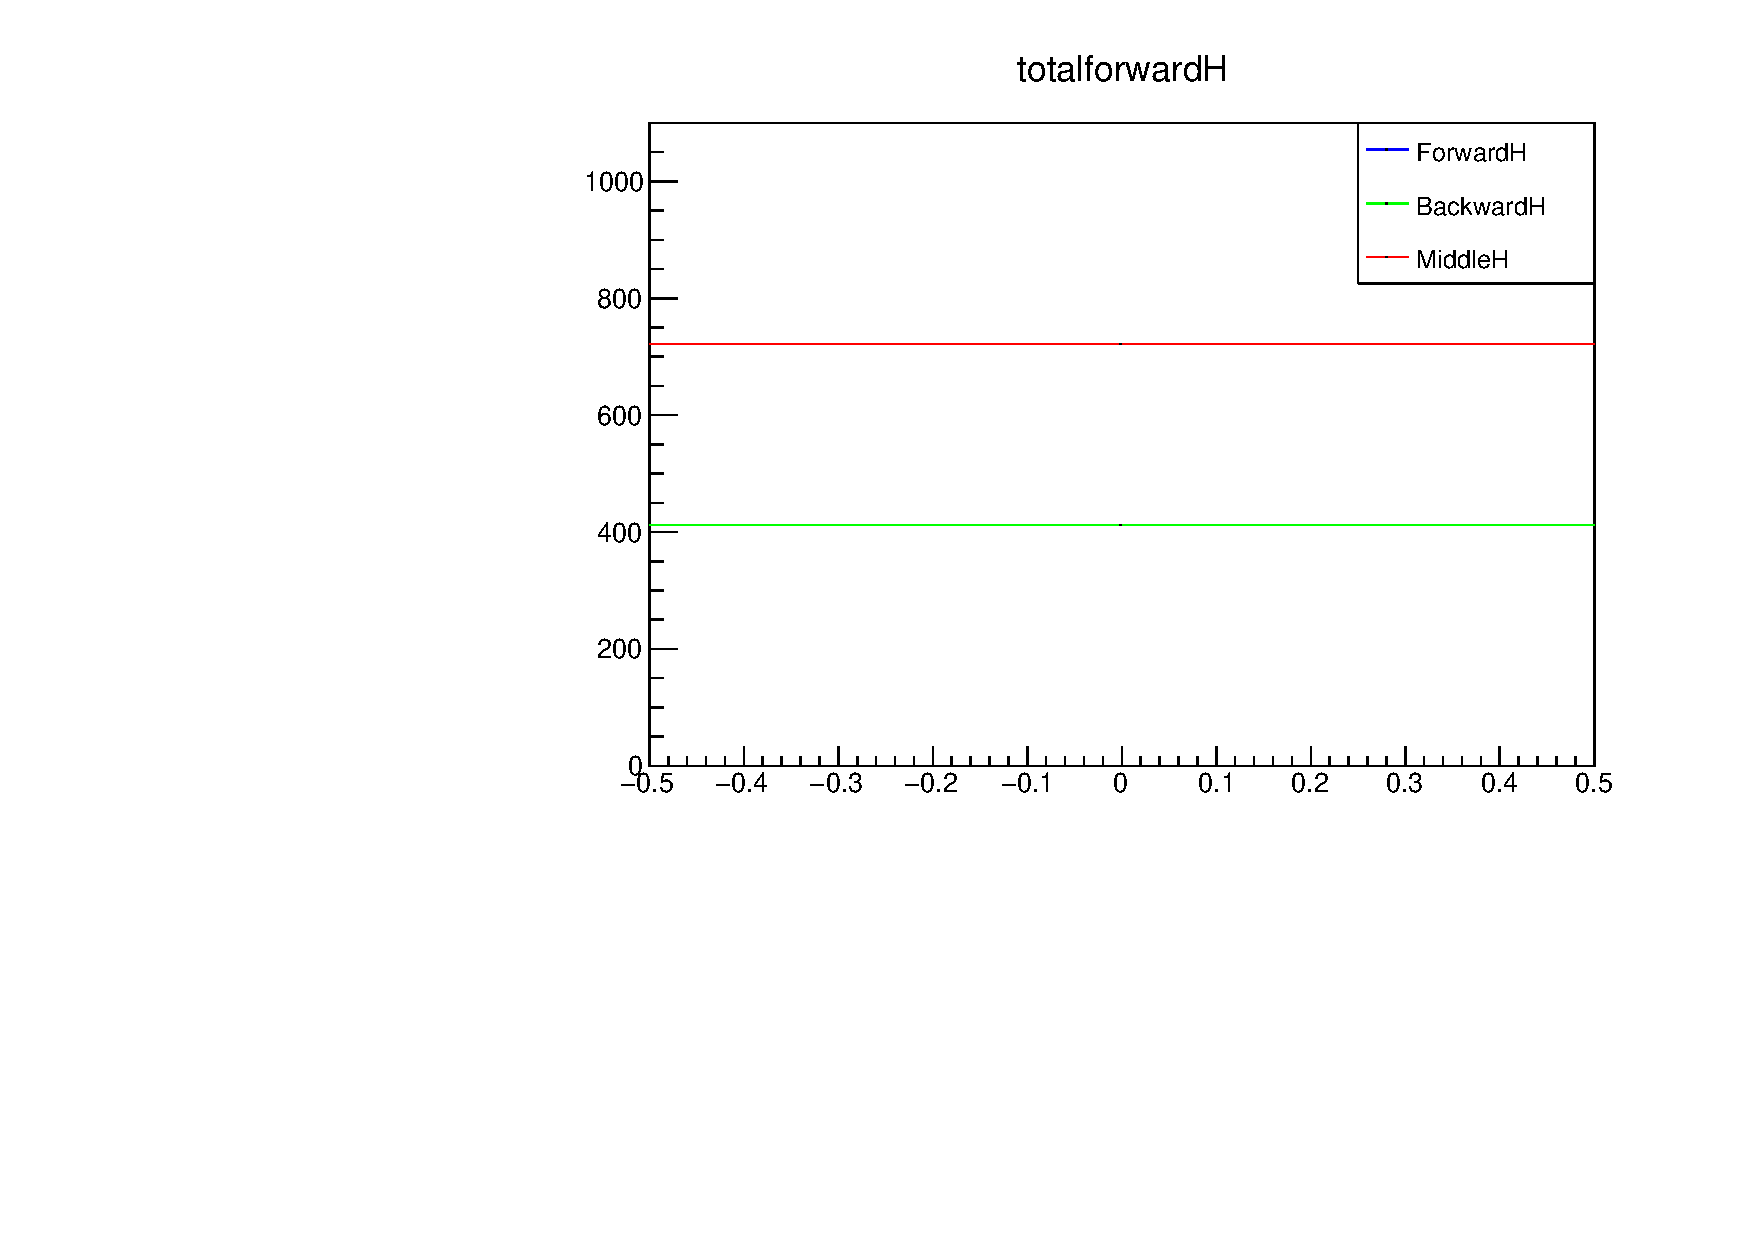
\includegraphics[scale=0.75]{Images/xsec_breakdown_ggh.pdf}
\caption{Cross-section breakdown in $gg \to ggH$ into forward Higgs production, backward Higgs production and central Higgs with infinite top mass.}
\label{fig:gg_crosssection}
\end{figure}

\begin{figure}[H]
\centering
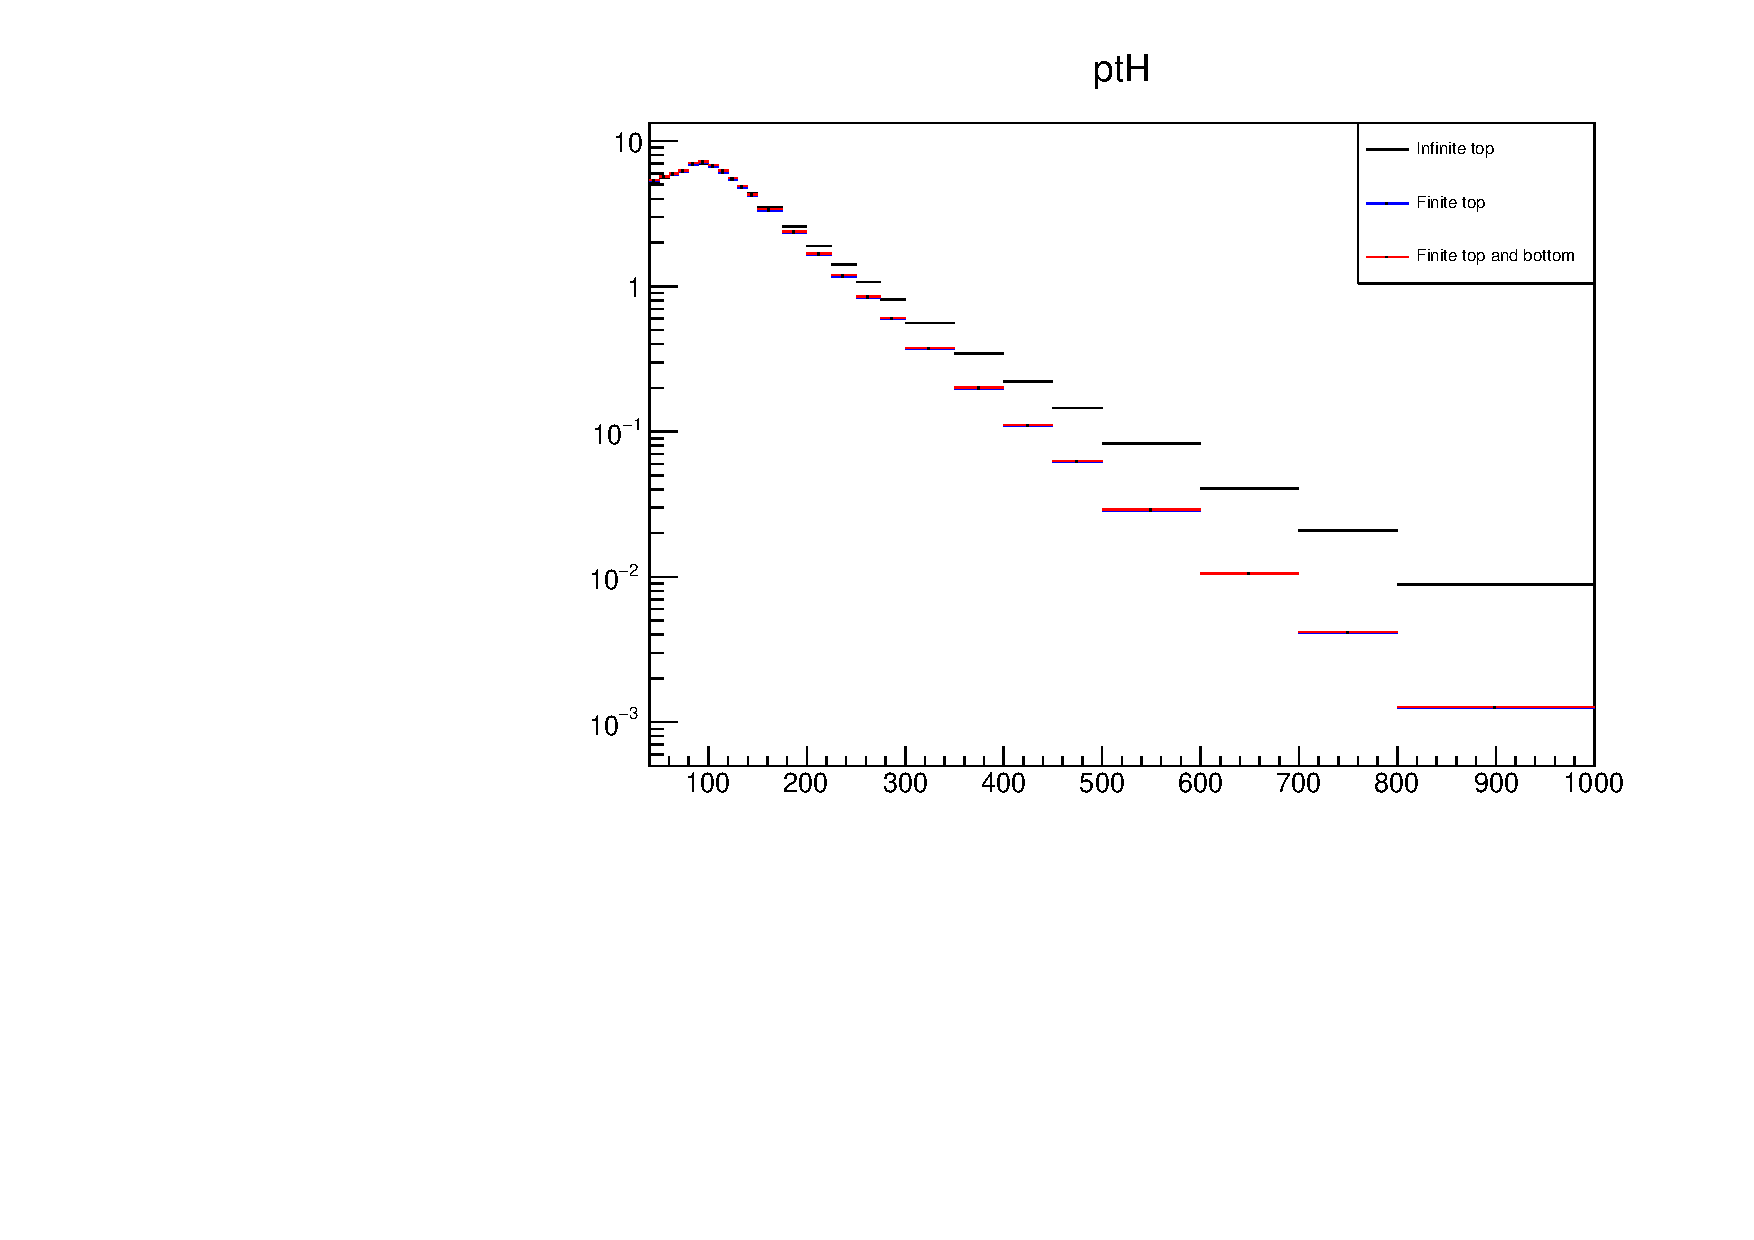
\includegraphics[scale=0.7]{Images/ptH_gg.pdf}
\caption{Comparison of infinite top mass, finite top mass and finite top plus finite bottom mass cross-sections in $gg \to ggH$, binned in Higgs $p_T$. }
\label{fig:pth_gg}
\end{figure}

\begin{figure}[H]
\centering
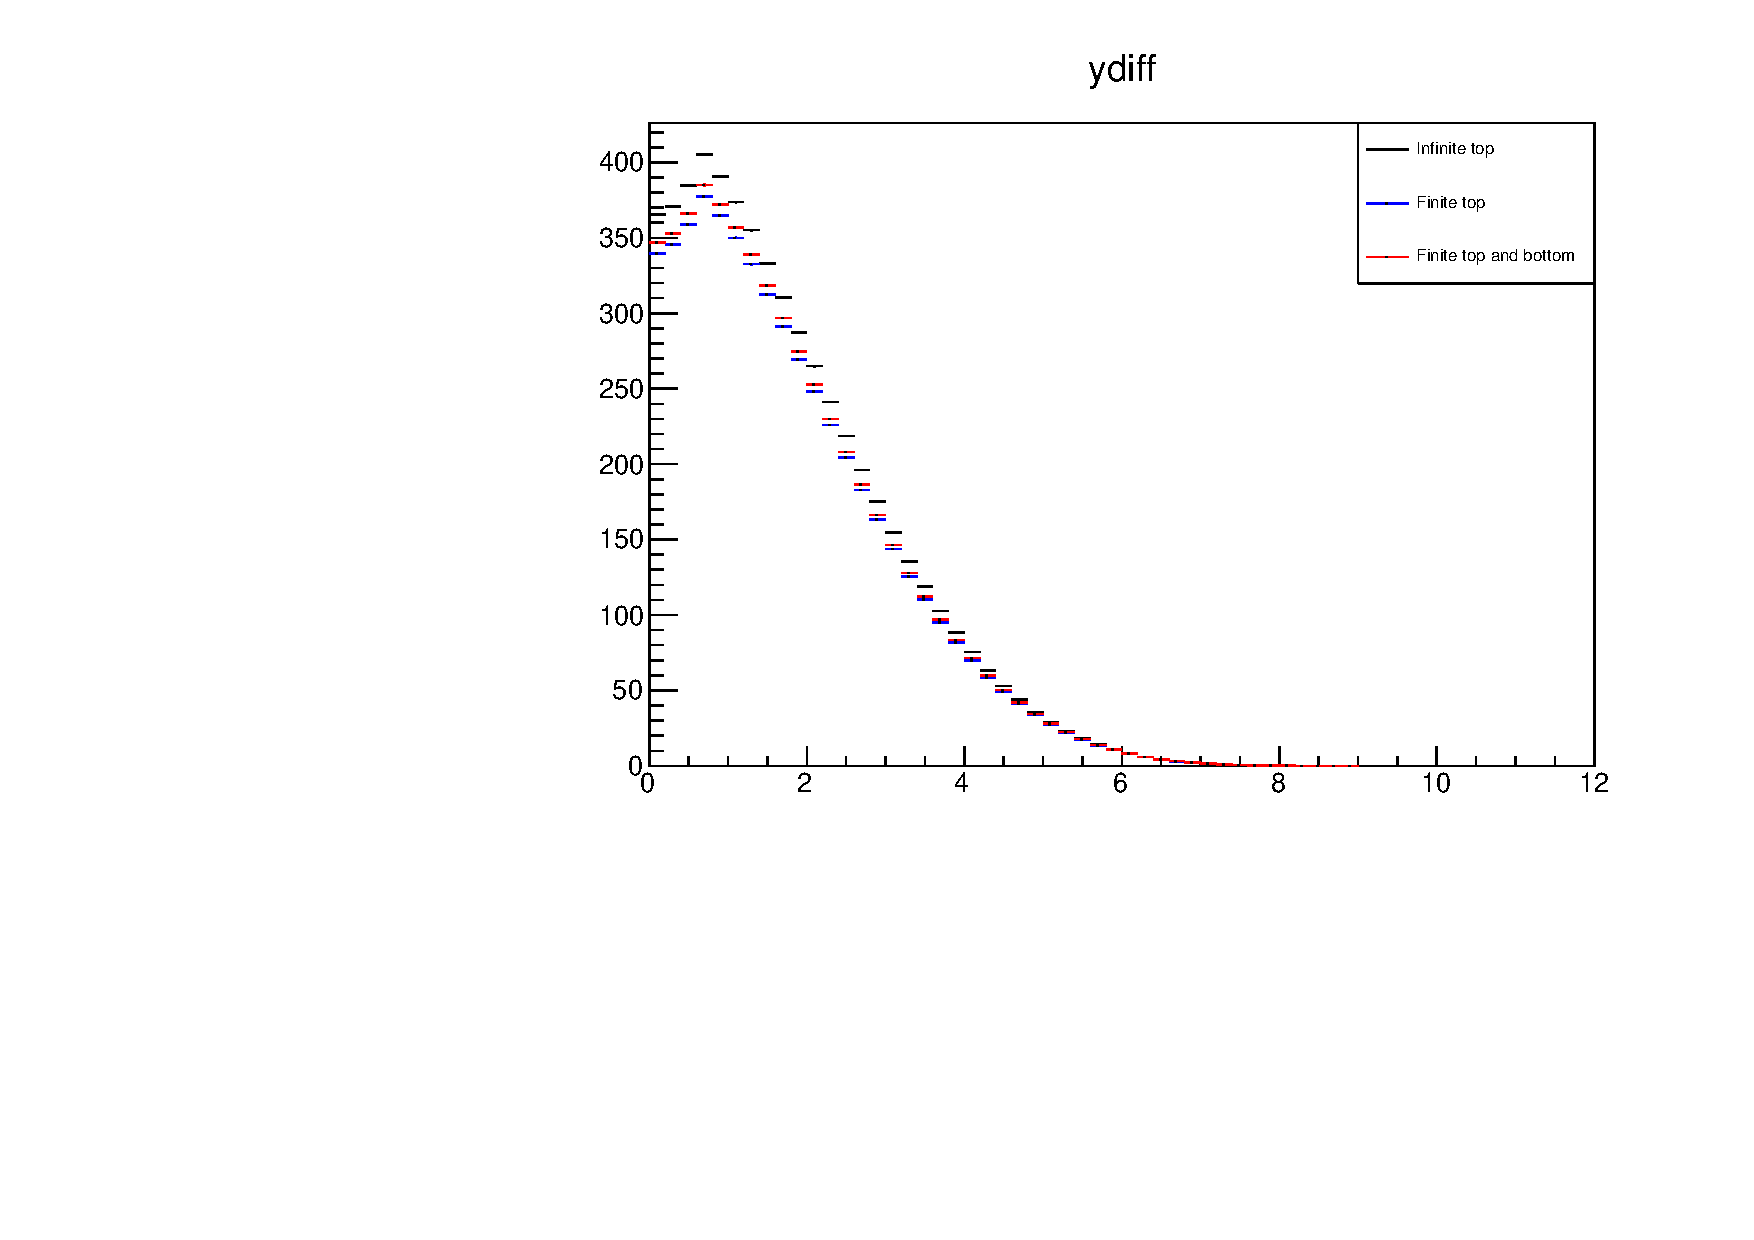
\includegraphics[scale=0.7]{Images/ydiff_gg.pdf}
\caption{Comparison of infinite top mass, finite top mass and finite top plus finite bottom mass cross-sections in $gg \to ggH$, binned in rapidity difference between the gluon and up quark.}
\label{fig:ydiff_gg}
\end{figure}
%\todo{All analysis plots need labels on axes}
We also investigate the effect of adding a third jet so as to perform a $gg \to gggH$ analysis. An interesting plot to show is, again, the Higgs $p_T$ as shown in figure \ref{fig:pth_gg_gggH}. We see a significant difference between the infinite top mass results and the finite top mass results in all bins -- strikingly, at low Higgs $p_T$. This would seem to contradict our prediction that low transverse scales imply that the effective theory is valid. The problem is that, in a three jet event, you can manufacture a situation whereby there is a large hierarchy between the transverse scales that enter the Higgs vertex. If instead we plot the cross-section as a function of the largest transverse scale that enters into this vertex, we should then once more again see the agreement in the low $p_T$ end. Figure \ref{fig:maxprop} shows this clearly. %\todo{Run analysis with full pp to H}

\begin{figure}[t]
\centering
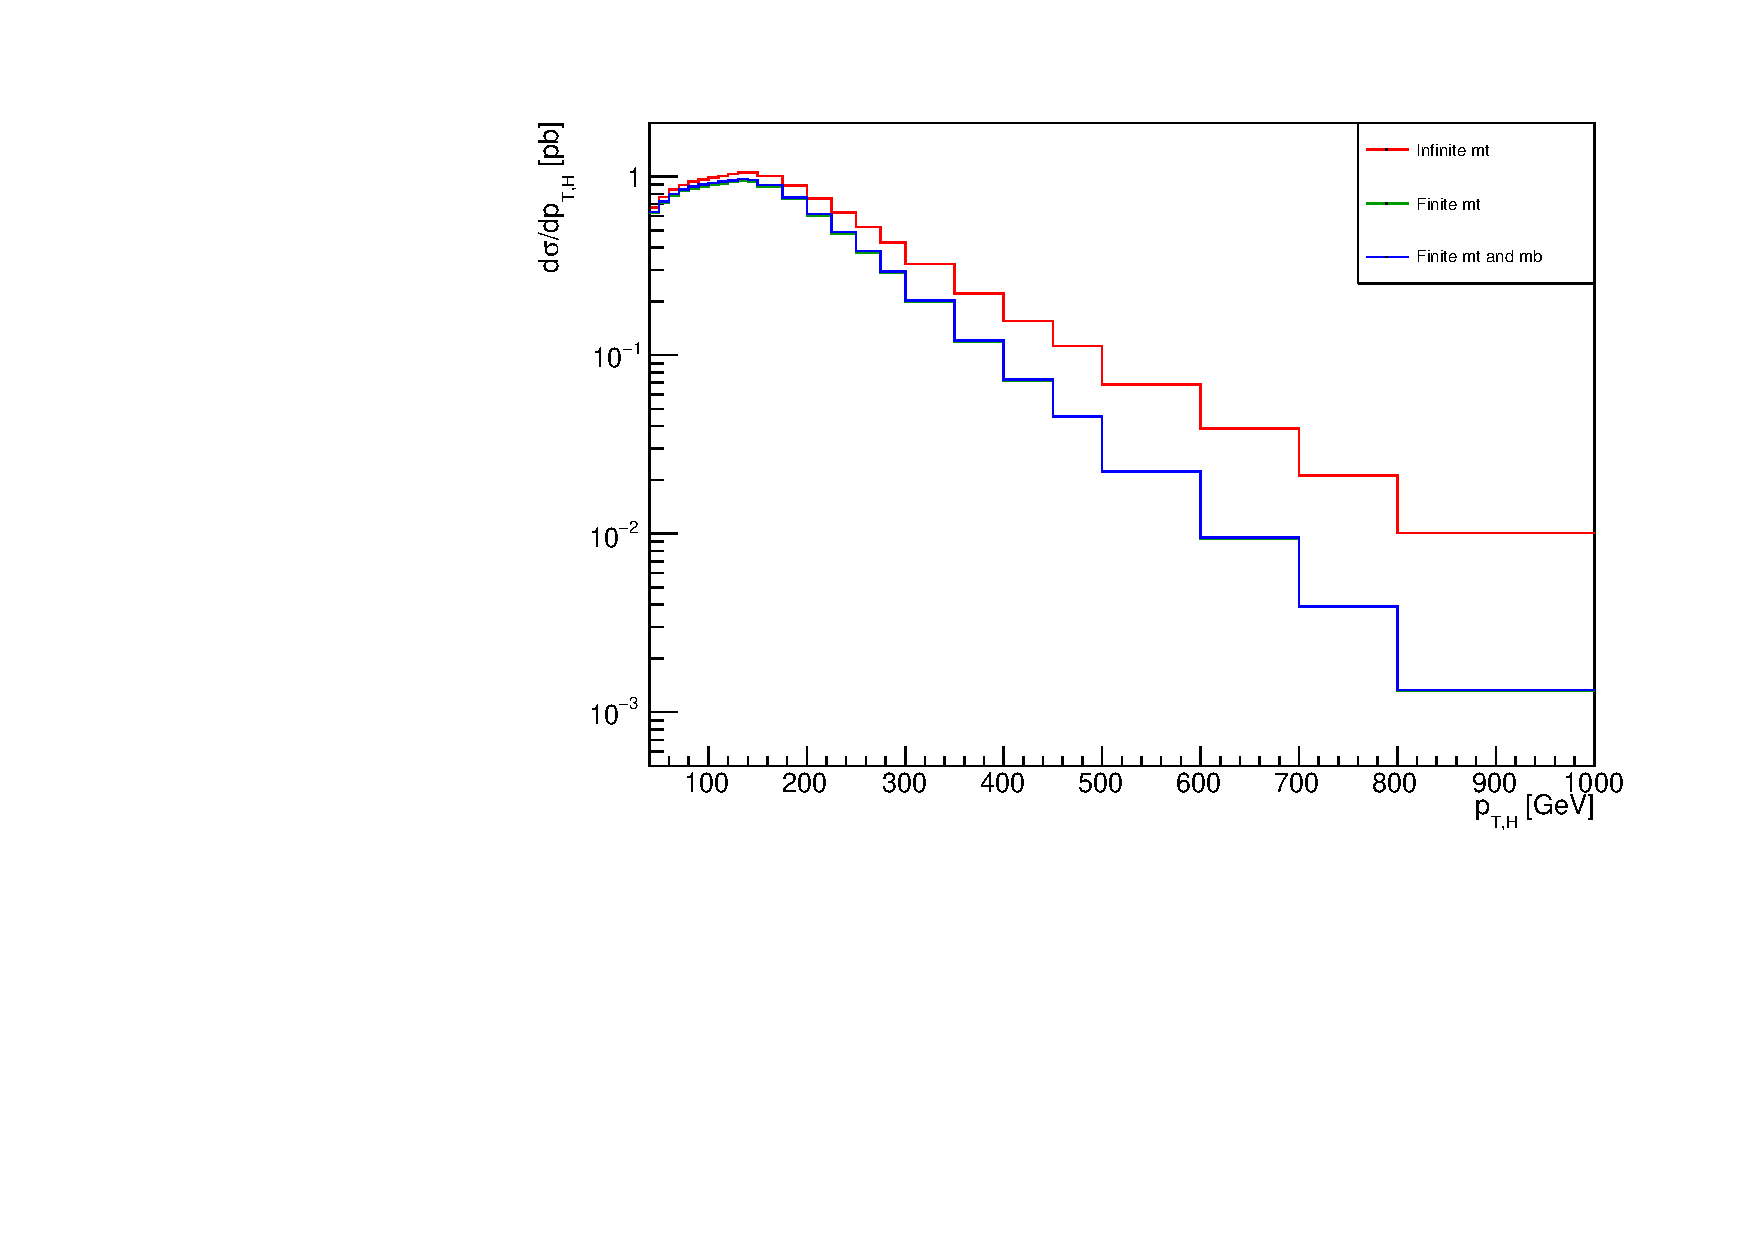
\includegraphics[scale=0.72]{Images/ptH_3j.pdf}
\caption{Comparison of infinite top mass, finite top mass and finite top plus finite bottom mass cross-sections in $gg \to gggH$, binned in Higgs $p_T$. }
\label{fig:pth_gg_gggH}
\end{figure}

\begin{figure}[H]
\centering
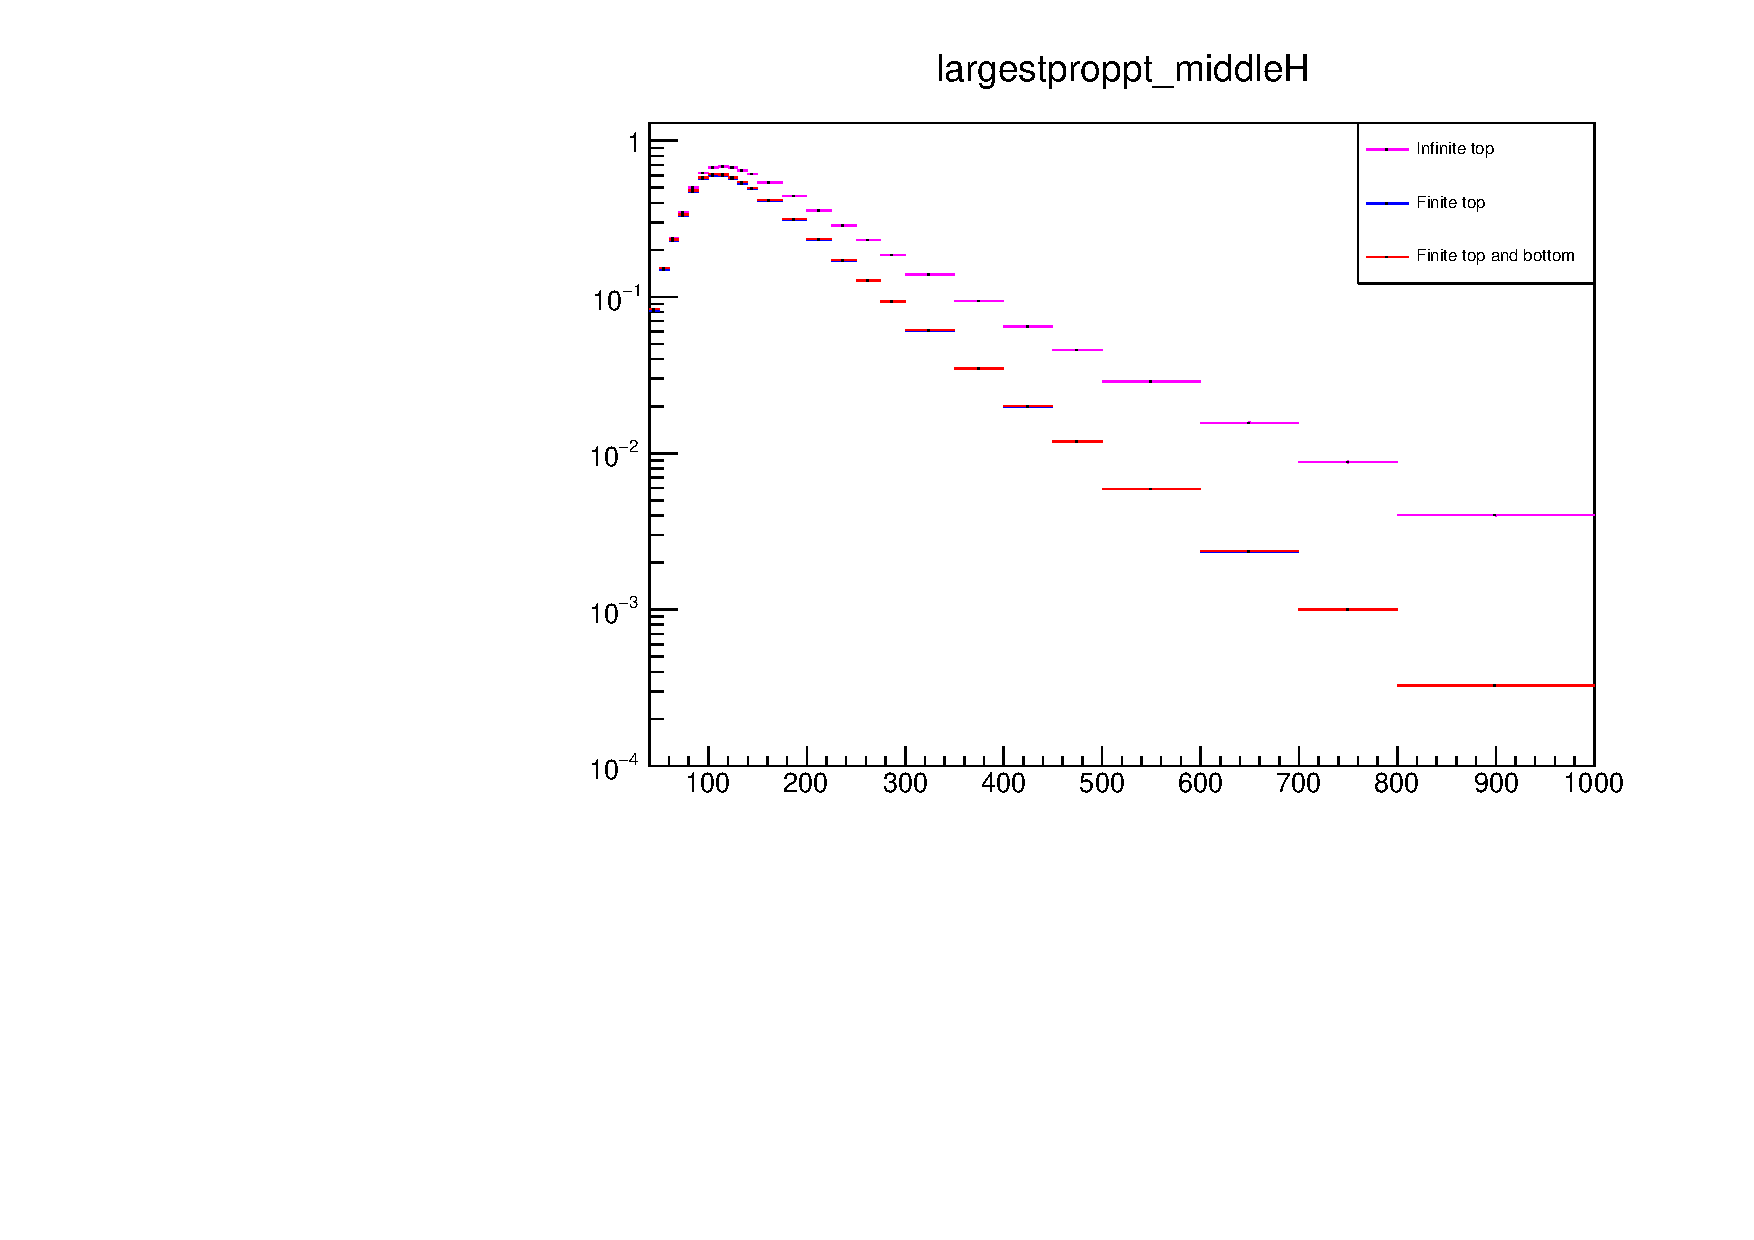
\includegraphics[scale=0.72]{Images/largestproppt.pdf}
\caption{Comparison of infinite top mass, finite top mass and finite top plus finite bottom mass cross-sections in $gg \to gggH$, binned in the maximum $p_T$ of a gluon entering into the Higgs vertex. }
\label{fig:maxprop}
\end{figure}

Unfortunately, there have so far not been many analyses of Higgs plus jets physics from the LHC and the ones that do exist focus on weak boson fusion rather than gluon fusion \cite{ATLAS2016}. For this reason, we are not yet able to compare these predictions to real data. We are, however, now in a prime position to provide predictions for any such data when it arrives. We conclude this section instead with an inclusive Higgs plus dijets prediction and again point out the difference between the full $m_t$ and infinite $m_t$ approaches. The $p_T$ spectra of the Higgs for this case is plotted in figure \ref{fig:hjj_ptH}, along with the ratio of the finite $m_t$ and finite $m_t + m_b$ lines to the infinite $m_t$ line. We see clearly that the distribution obtained with the effective theory is significantly different. The same is true if we look at the $\Delta y$ distribution, shown in figure \ref{fig:hjj_dy}.

\begin{figure}[t]
\centering
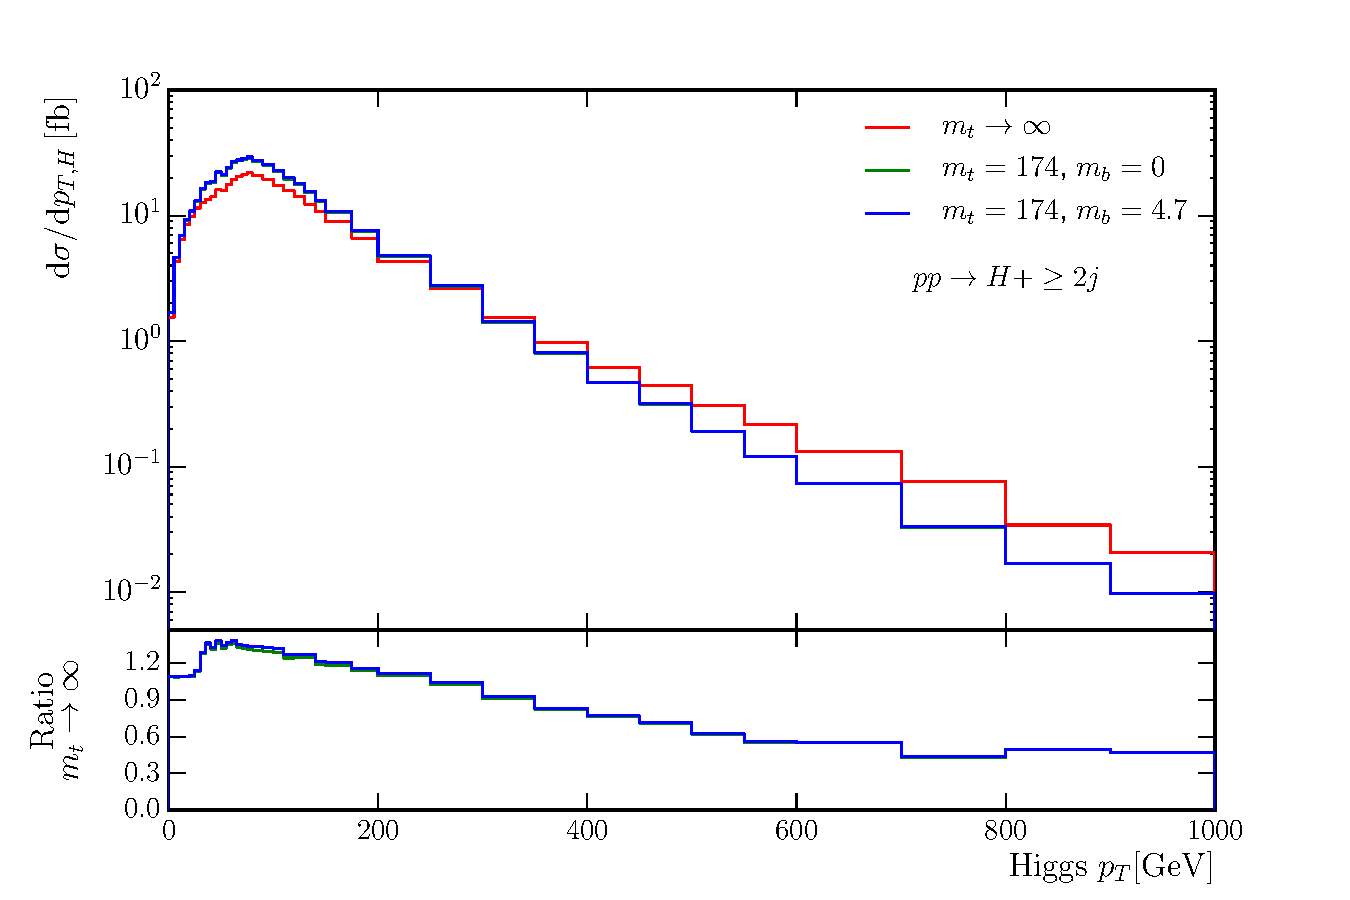
\includegraphics[scale=0.64]{Images/Higgs_Plots/pth_compare_all.pdf}
\caption{Comparison of infinite top mass, finite top mass and finite top plus finite bottom mass cross-sections in $pp \to H+\geq2j$, binned in the $p_T$ of the Higgs.}
\label{fig:hjj_ptH}
\end{figure}

\begin{figure}[t]
\centering
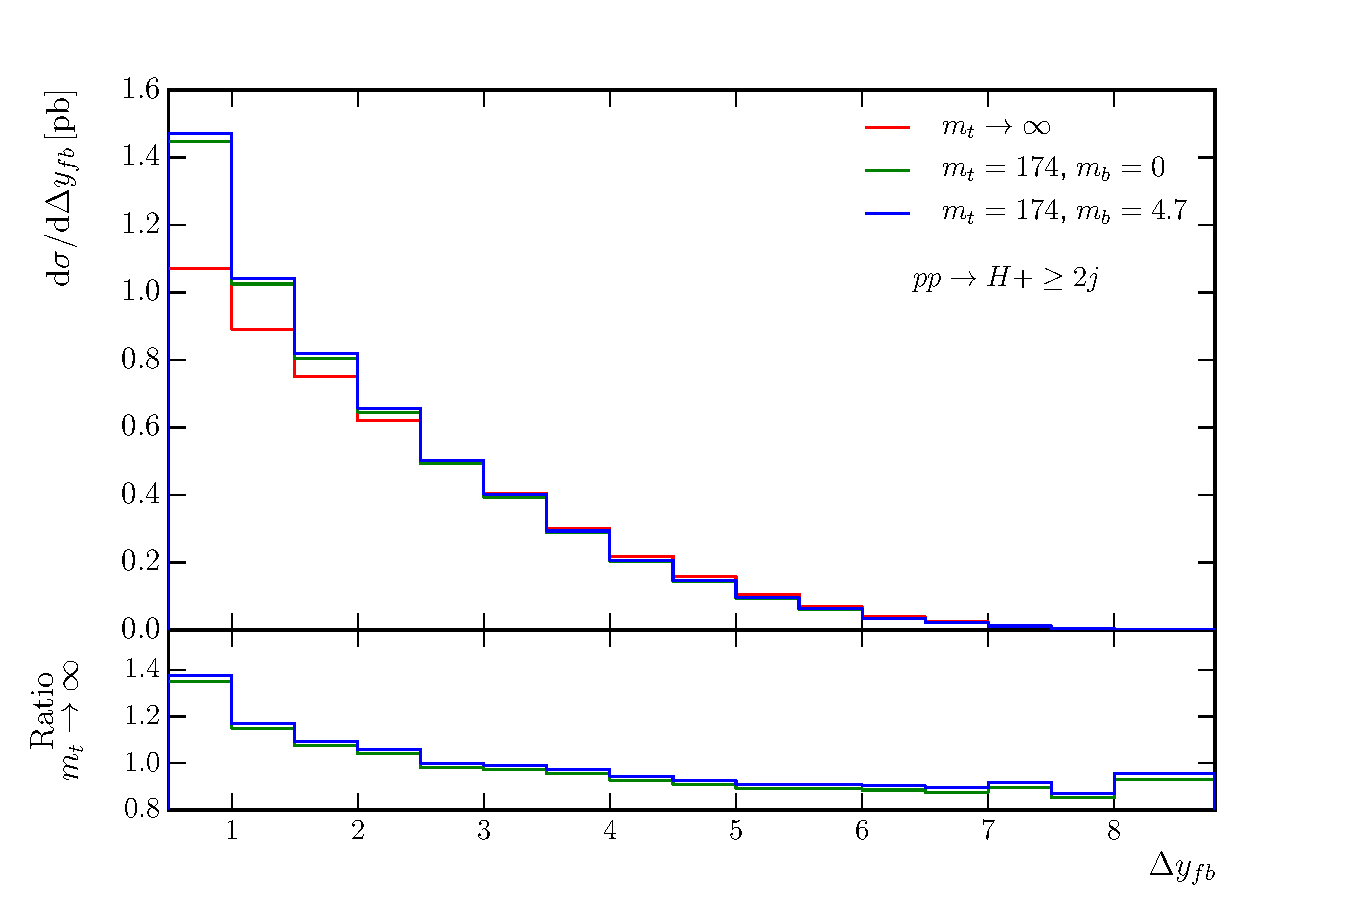
\includegraphics[scale=0.64]{Images/Higgs_Plots/dyfb_compare_all.pdf}
\caption{Comparison of infinite top mass, finite top mass and finite top plus finite bottom mass cross-sections in $pp \to H+\geq2j$, binned in the rapidity difference between the most forward/backward jets.}
\label{fig:hjj_dy}
\end{figure}

In all of these distributions, we see that the addition of a bottom loop has a small overall effect. This would suggest that the Higgs + 1 jet studies of \cite{Lindert2017} and \cite{Grazzini2013}, where a sizeable difference was seen, is an effect of having only one jet accompanying the Higgs. 

\section{Summary}
In his chapter, we have discussed how HEJ can be extended to describe processes involving the production of a Higgs boson along with two or more jets. We discussed how, due to the added complexity of calculating loop diagrams, many fixed order approaches to the description of such amplitudes employ the infinite top mass limit. Using this as a first approximation, we showed how the HEJ amplitude looks in this limit by a simple redefinition of the current object. 

From here, we argued that the employment of the infinite top mass limit is not required in HEJ: the High Energy and infinite top mass limits commute. Taking the simple example of $qQ \to qHQ$, we showed how simple it is for HEJ to keep the full finite quark mass effects in its amplitudes. By considering the limit where a Higgs boson is produced outside of a gluon, the bulk of the chapter describes the more involved calculation of the HEJ amplitude for this case, again keeping full finite quark mass effects. 

Analysis of this amplitude over the LHC phase space confirmed previously known results: namely, that the presence of a large dijet invariant mass does little to invalidate the infinite top mass limit. Instead, the relevant variable is the transverse scales that feature in the quark loop, where we saw the striking result that at high values of the Higgs $p_T$, the difference between the effective and full theories is a factor of two. 

The main result of this work is that HEJ is now able to provide predictions for Higgs plus $\geq 2$ jet processes with full top and bottom mass effects included. Although leading order results are known for the full theory with small multiplicities of jets \cite{DelDuca2001a, Neumann2016}, HEJ's ability to resum the amplitude to all orders in $\alpha_s$ whilst keeping the full dependence on the quark masses is unique. 

%\todo{Mention no compare with data because lack of it}